\documentclass[10pt]{article}

\usepackage{array}
\usepackage{amsthm}
\usepackage{amsmath}
\usepackage{amssymb}
\usepackage{amsfonts}
\usepackage{stmaryrd}
\usepackage{tikz}
\usepackage{comment}
\usepackage{xspace}
\usepackage{makeidx}
\usepackage{stackengine}
\usepackage{ifthen}
\usepackage{listofitems}
\usepackage{graphicx}
\usepackage[final]{listings}
\usepackage{hyperref}
\usepackage{enumitem}

\graphicspath{ {.} }
\lstset{language=Java,
  commentstyle=\color{brown},
  keywordstyle=\color{blue},
  stringstyle=\color{red},
  basicstyle=\ttfamily}

\lstdefinelanguage{ddlog}{
  language=Java, % we base it on Java, just for comments
  morekeywords={input, output, typedef, relation, typedef, bool, not,
    string, bit, extern, function, var, for, match, skip, in, integer, % not really in DDlog
    Aggregate, FlatMap},
  deletestring=[b]{'}
}
\hypersetup{
  colorlinks   = true,    % Colours links instead of ugly boxes
  urlcolor     = blue,    % Colour for external hyperlinks
  linkcolor    = blue,    % Colour of internal links
  citecolor    = red      % Colour of citations
}
\hypersetup{final}

\usetikzlibrary{shapes, arrows.meta, positioning}
\tikzstyle{block} = [draw, fill=white, rectangle]

\input{matrix}
\theoremstyle{definition}
\newtheorem{theorem}{Theorem}[section]
\newtheorem{lemma}[theorem]{Lemma}
\newtheorem{corollary}[theorem]{Corollary}
\newtheorem{definition}[theorem]{Definition}
\newtheorem{proposition}[theorem]{Proposition}
\newtheorem{example}[theorem]{Example}
\newtheorem{algorithm}[theorem]{Algorithm}

\newcommand{\secref}[1]{Section~\ref{#1}}  % reference to a section
\newcommand{\refsec}[1]{\secref{#1}}
% Used when a term is first defined.  Adds the term to the index.
\newcommand{\defined}[1]{\textbf{#1}\index{#1}}
\newcommand{\zr}{$\Z$-set\xspace}
\newcommand{\zrs}{$\Z$-sets\xspace} % plural
\newcommand{\means}[1]{\ensuremath{\llbracket #1 \rrbracket}}
\newcommand{\code}[1]{\mbox{\texttt{#1}}}
\newcommand{\Z}{\mathbb{Z}}  % integers
\newcommand{\N}{\mathbb{N}}  % naturals
\newcommand{\B}{\mathbb{B}}  % Booleans
\newcommand{\norm}[1]{\| #1 \|} % norm; requires math mode
% stream with elements of a given type
\newcommand{\stream}[1]{\ensuremath{\mathcal{S}_{#1}}}
% finite stream with elements of a given type (zero almost everywhere)
\newcommand{\streamf}[1]{\ensuremath{\overline{\mathcal{S}_{#1}}}}
\newcommand{\zm}{\ensuremath{z^{-1}}} % stream delay operator
\ifthenelse{\equal{1}{1}}{ % allows switching to mathit/mathcal
\newcommand{\I}{\mathcal{I}}  % stream integration
\newcommand{\D}{\mathcal{D}}  % stream derivative
}{
\newcommand{\I}{\mathit{I}}  % stream integration
\newcommand{\D}{\mathit{D}}  % stream derivative
}
\newcommand{\inc}[1]{{#1}^{\Delta}}
\newcommand{\dbsp}{DBSP\xspace}
\newcommand{\distinct}{\mathit{distinct}}  % distinct operator
% set with elements of given type
\newcommand{\set}[1]{\mathit{set}_{#1}}
\newcommand{\id}{\ensuremath{\mathit{id}}} % identity function
\newcommand{\isset}{\mbox{isset}}
\newcommand{\ispositive}{\mbox{ispositive}}
\newcommand{\defn}{\stackrel{\textrm{\scriptsize def}}{=}}
\newcommand{\map}{\mbox{map}}
\newcommand{\fix}[2]{\mbox{fix}\,#1.#2}
\newcommand{\lift}[1]{{\uparrow}#1}
\newcommand{\rew}{\ensuremath{\mapsto}} % rewriting
\newcommand{\birew}{\ensuremath{\mapsfrom\!\mapsto}} % bidirectional rewriting
\newcommand{\pair}[2]{\ensuremath{\langle #1,#2 \rangle}} % pairing
\newcommand{\zpp}[1]{\mbox{zpp}(#1)}
\newcommand{\sv}[1]{ % simple stream value, supplied as a space-separated list of 5 values
\setsepchar{ }
\readlist\arg{#1}
{[}
\begin{array}{cccccc}
    \arg[1] & \arg[2] & \arg[3] & \arg[4] & \arg[5] & \cdots
\end{array}
{]}
}

\newcommand{\st}{\;|\;}
\newcommand\Hookarrowleft[1]{\ensuremath{\stackrel{\curvearrowleft}{#1}}}

\newcommand{\cut}[2]{#1|_{_{\leq #2}}}
\newcommand{\scut}[2]{#1|_{_{< #2}}}


\setlength{\marginparwidth}{4cm}
\newcommand{\scream}[2]{\marginpar{\footnotesize \textbf{#1}: #2}}
\newcommand{\val}[1]{\scream{VAL}{#1}}
\newcommand{\mihai}[1]{\scream{MIHAI}{#1}}
\newcommand{\leonid}[1]{\scream{LEONID}{#1}}

\title{\dbsp: A Language for Expressing Incremental View Maintenance
  for Rich Query Languages --- full version}
\author{
Mihai Budiu \\ VMware Research \and
Frank McSherry \\ Materialize Inc. \and
Leonid Ryzhyk \\ VMware Research \and
Val Tannen \\ University of Pennsylvania
}

\makeindex
\begin{document}

\maketitle

\begin{abstract}
Incremental view maintenance has been for a long time a central problem of database theory.
Many solutions have been proposed for restricted classes of database languages,
such as the relational algebra, or Datalog.  These techniques do not naturally generalize to
richer languages.  In this paper we give a general
solution to this problem in 3 steps: (1) we describe a simple but expressive language
called \dbsp for describing computations over data streams; (2) we give a general algorithm for
solving the incremental view maintenance problem for arbitrary \dbsp programs, and (3) we show
how to model several classes of database query languages (including relational queries,
grouping and aggregation, and recursion) using \dbsp.  \dbsp
can be used to model other interesting query languages, including
streaming aggregation queries, non-monotonic recursion, and queries on nested relations.
As a consequence, we obtain efficient
incremental view maintenance techniques for all these rich languages.
\end{abstract}

\begin{quote}
This document is work in progress.  It contains a formal specification
of the \dbsp language, proofs of the theoretical results, and the
specification of the implementation of several query languages in
\dbsp.
\end{quote}

\tableofcontents

\section{Introduction}\label{sec:ntro}

In this paper we present a simple mathematical theory for modeling
streaming and incremental computations.  This model has immediate
practical applications in the design and implementation of streaming databases
and incremental view maintenance.  Our model is based on mathematical formalisms 
used in discrete digital signal processing (DSP)~\cite{rabiner-book75},
but we apply it to database computations.  
Thus, we have called it ``\dbsp''.  

We borrow the following concepts from DSP: discrete signal streams, the
delay operator $\zm$, time-invariance (also called shift-invariance), causality,
strictness, z-transforms, integration, and differentiation.  The concept of
linear transformation is also central to DSP.

\dbsp is also inspired from Differential 
Dataflow~\cite{mcsherry-cidr13} (DD), and started as an attempt to provide a simpler
formalization of DD than the one of Abadi et al.~\cite{abadi-fossacs15} 
(as discussed in \secref{sec:related}), but has evolved behind that purpose.

The core concept of \dbsp is the \emph{stream}: a stream $s$ with type 
$\stream{A}$ maps ``time'' moments $t\in\N$ 
to values $s[t]$ of type $A$; think of it as an "infinite vector".
A streaming computation is a function that
consumes one or more streams and produces another stream.  We depict
streaming computations with typical DSP box-and-arrow diagrams (also called ``circuits''),
where boxes are computations and streams are arrows, as in the diagram from Figure~\ref{fig:stream},
which shows a stream operator $T$ consuming two input streams $s_0$ and $s_1$ 
and producing one output stream $s$.

\begin{figure}
\begin{center}
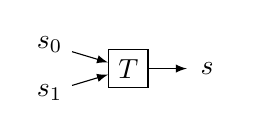
\begin{tikzpicture}[auto,>=latex,minimum width=.5cm]
  \node[] (input0) {$s_0$};
  \node[below of=input0,node distance=.3cm] (dummy) {};
  \node[below of=dummy,node distance=.3cm] (input1) {$s_1$};
  \node[block, right of=dummy] (T) {$T$};
  \node[right of=T] (output) {$s$};
  \draw[->] (input0) -- (T);
  \draw[->] (input1) -- (T);
  \draw[->] (T) -- (output);
\end{tikzpicture}
\vspace{-.2cm}
\caption{A simple streaming circuit that consumes two streams and produces one stream.\label{fig:stream}}
\end{center}
\end{figure}

We generally think of streams as sequences of \emph{small} values,
and we will use them in this way.
However, we make a leap of imagination and also treat a \emph{whole database} as a stream value.
What is a stream of databases?  It is a \emph{sequence of database
snapshots}.  We model the time-evolution of a database $DB$ as a
stream $DB \in \stream{SCH}$, where $SCH$ is the database schema.
Time is not the wall-clock time, but essentially a counter
of the \emph{sequence of transactions} applied to the database. 
Since transactions are linearizable,
they have a total order, which defines a linear time $t$ dimension:
the value of the stream $DB[t]$ is the snapshot of the 
database contents after $t$ transactions have been applied.  We assume
that $DB[0] = 0$, i.e., the database starts empty.

Database transactions also form a stream $T$, a stream of \emph{changes},
or \emph{deltas} that are applied to our database.   
The database snapshot at time $t$ is the cumulative result of applying all 
transactions in the sequence up to $t$: $DB[t] = \sum_{i \leq t} T[i]$.
The operation of adding up all changes is \emph{stream integration}.
The following diagram expresses this relationship using the $\I$ operator for 
stream integration:

\begin{center}
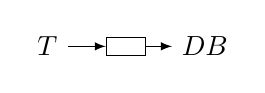
\begin{tikzpicture}[auto,>=latex,minimum width=.5cm]
  \node[] (input) {$T$};
  \node[block, right of=input] (I) {$\I$};
  \node[right of=I] (output) {$DB$};
  \draw[->] (input) -- (I);
  \draw[->] (I) -- (output);
\end{tikzpicture}
\end{center}

Conversely, we can say that transactions are the \emph{changes} of a database, and write
$T = \D(DB)$.  Stream differentiation, denoted by $\D$, 
is an operation that computes the changes of a stream, and is the 
inverse of stream integration.  \secref{sec:streams}
precisely defines streams, integration and differentiation, and analyzes
their properties. 

Let us apply these concepts to view maintenance.
Consider a database $DB$ and a query $Q$ defining a view $V$ as a function
of a database snapshot $V = Q(DB)$.  Corresponding to the stream of database snapshots
$DB$ we have a \emph{stream of view snapshots}: $V[t]$ is the
view's contents after the $t$-th transaction has been applied.  We show this
relationship using the following diagram:

\begin{center}
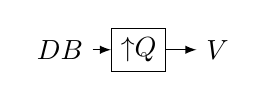
\begin{tikzpicture}[auto,>=latex,minimum width=.5cm]
  \node[] (input) {$DB$};
  \node[block, right of=input] (I) {$\lift{Q}$};
  \node[right of=I] (output) {$V$};
  \draw[->] (input) -- (I);
  \draw[->] (I) -- (output);
\end{tikzpicture}
\end{center}

The symbol $\lift{Q}$ (the ``lifting'' of $Q$) shows that the query $Q$ is applied
pointwise to every element of the stream of database snapshots $DB$.  We say that
$\lift{Q}$ is a ``streaming query'' since it operates on a stream of values.
The incremental view maintenance problem requires an algorithm to  
compute the stream $\Delta V$ of \emph{changes} of the view $V$, i.e., $\D(V)$,
as a function of the stream $T$.  
By chaining these definitions together we get the following \defined{fundamental equation}
of the view maintenance problem: $\Delta V = \D(\lift{Q}(DB)) = \D(\lift{Q}(\I(T)))$,
graphically shown as:

\begin{center}
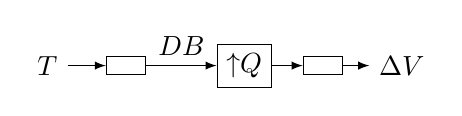
\begin{tikzpicture}[auto,>=latex,minimum width=.5cm]
  \node[] (input) {$T$};
  \node[block, right of=input] (I) {$\I$};
  \node[block, right of=I, node distance=1.5cm] (Q) {$\lift{Q}$};
  \node[block, right of=Q] (D) {$\D$};
  \node[right of=D] (output) {$\Delta V$};
  \draw[->] (input) -- (I);
  \draw[->] (I) -- node (db) {$DB$} (Q);
  \draw[->] (Q) -- (D);
  \draw[->] (D) -- (output);
\end{tikzpicture}
\end{center}

This definition is the subject of Section~\ref{sec:incremental}.
The notion can be generalized to more general streaming queries
$S: \stream{A} \to \stream{B}$ that are richer than lifted pointwise queries $Q$.
The incremental version of streaming query $S$ is denoted by $\inc{S}$ and is defined
according to the above equation, which can also be written as: $\inc{S} = \D \circ S \circ \I$. 

It is generally assumed that the changes to a dataset are much smaller than
the dataset itself; thus, computing on streams of changes may
produce significant performance benefits.

Applying the query \emph{incrementalization} operator $S \mapsto \inc{S}$ constructs
a query that computes directly on changes; however, the resulting query is no more
efficient than a query that computes on the entire dataset, because it uses an
integration operator to reconstitute the full dataset.
\secref{sec:incremental} shows algebraic properties of the $\inc{\cdot}$ operator 
that can used to optimize the implementation of $\inc{S}$:

\begin{enumerate}[label=\textbf{(\arabic*)}]
\item The first property is that many classes of primitive operations have very efficient incremental
versions.  In particular, linear queries have the property $Q = \inc{Q}$.  Almost all
relational and Datalog queries are based on linear operators.  Thus, the incremental version
of such queries can be computed in time proportional to the size of the changes.  Bilinear 
operators (such as joins) have a more complex implementation, which nevertheless still performs 
work proportional to the size of the changes, but require storing an amount of data proportional
to the size of the relations.

\item The second key property is the chain rule:
$\inc{(S_1 \circ S_2)} = \inc{S_1} \circ \inc{S_2}$.  This rule gives the incremental
version of a complex streaming query as a composition of incremental versions of its components.
It follows that we can implement any incremental query as a composition of primitive
incremental queries, \emph{all of which perform work proportional to the size of the changes}.
\end{enumerate}

While this machinery is sufficient to express the whole relational algebra and
recursive queries, it is not sufficient to incrementalize recursive queries.
So in \refsec{sec:nested} we extend \dbsp to operate on nested streams.

First, in \secref{sec:stream-intro-elim} we introduce two additional operators: $\delta_0$
creates a stream from a scalar value, and $\int$ creates a scalar value from a stream.  
These operators can be used to implement computations with \code{while} loops.
So, in addition to modelling changing inputs and database, we also
use streams as a model for sequences of \emph{consecutive values of loop
iteration variables}.  This model will enable us to implement recursive queries.

In \secref{sec:nested} we use \dbsp to model computations on nested streams, where each 
value of a stream is another stream.  With this extension \dbsp becomes rich enough to
model incremental streaming recursive queries.

Armed with (a) a language that can express many classes of queries and
(b) a  general theory of incremental computation, we proceed in a sequence of
sections to apply these techniques to richer and richer query languages.

In \secref{sec:relational}  
we show how to model relational queries in \dbsp.  This immediately gives
us a general algorithm to compute the incremental version of any relational query.
These results are well-known, but they are cleanly modeled by \dbsp.

\secref{sec:recursive} shows how recursive queries can be implemented in \dbsp.  
This allows us to define in \refsec{sec:inc-recursive} \emph{incremental streaming computations 
for recursive programs}.  As a consequence we derive a universal algorithm for incrementalizing
arbitrary streaming Datalog programs.

\secref{sec:extensions} shows how other classes of powerful query languages can
be modeled in \dbsp: streaming window queries, queries on nested relations (such as grouping),
non-monotone recursive queries, and while-relational queries. 

Interestingly, the incrementalization algorithm can applied to all \dbsp programs.

\dbsp is a \textbf{simple} language: 
the basic  \dbsp streaming model is built essentially from two elementary 
mathematical operators: lifting $\lift$ and delay $\zm$.
The nested streams model adds two additional operators, $\delta_0$ for 
stream construction and $\int$ for destruction.

Despite its simplicity, \dbsp is also \textbf{expressive}, and we show how many useful
query languages can be modeled in \dbsp.

\dbsp is \textbf{mathematically abstract}: the two core concepts of 
(1) streaming computations, and (2) incremental computations
are completely abstract, since they work over any algebraic group structure.  
By instantiating the group structure with the real numbers $\mathbb{R}$, 
we get traditional signal processing systems.  By substituting
for the group structure \zrs we obtain streaming incremental computations over databases. 

\subsection{Notations used in this paper}

The following tables summarize the mathematical notations used in the rest of this paper.

\noindent
\begin{center}
\begin{tabular}{|c|p{10cm}|} \hline
%\textbf{Notation} & \textbf{Meaning} \\ \hline

\multicolumn{2}{|c|}{General notations} \\ \hline
$\Z$ & The ring of integer numbers \\
$\N$ & The set of natural numbers $0, 1, 2, \ldots$ \\
$\B$ & The set of Boolean values \\
$[n]$ & The natural numbers between 0 and $n-1$ \\
$\id$ & The identity function over some domain $\id: A \to A$, $\id(x) = x$ \\
$\means{Q}$ & Semantics of query (function) $Q$ \\
$\pair{a}{b}$ & The pair containing values $a$ and $b$ \\
fst$(p)$ & The operator that returns the first value of a pair $p$ \\
snd$(p)$ & The operator that returns the second value of a pair $p$ \\
$a \mapsto b$ & The function that maps $a$ to $b$ and everything else to 0 \\          
$\lambda x.M$ & An anonymous function with argument $x$ and body $M$ \\
$\fix{x}{f}$ & The (unique) solution (fixed point) of the equation $f(x) = x$ \\
\hline
\end{tabular}

\noindent
\begin{tabular}{|c|p{10cm}|} \hline
\multicolumn{2}{|c|}{Streams} \\ \hline
$\stream{A}$ & The set of streams with elements from a group $A$; $\stream{A} = \{ f \,|\, f : \N \to A \}$ \\
$\streamf{A}$ & Streams with elements from a group $A$ that are 0 almost everywhere \\
$s[t]$ & The $t$-th element of a stream; $s[t] = s(t)$ \\
$\lift{f}$ & An operator applied to a function $f: A \to B$ to produce a function $\lift{f}: \stream{A} \to \stream{B}$
           operating pointwise \\
$\zpp{f}$ & $\zpp{f}$ iff $f(0) = 0$ for $f: A \to B$ for $A, B$ groups \\
$\zm$ & The stream delay operator $\zm: \stream{A} \to \stream{A}$, that outputs a 0 followed by the input stream \\
$\I$ & The stream integration operator $\I: \stream{A} \to \stream{A}$ \\
$\D$ & The stream differentiation operator $\D: \stream{A} \to \stream{A}$ \\
$\inc{Q}$ & The incremental version of an operator $\inc{Q} = \D \circ Q \circ \I$ \\
$\cut{s}{t}$ & A stream that has the same prefix as $s$ up to $t$, then it is all 0s \\
$\scut{s}{t}$ & A stream that has the same prefix as $s$ up to $t-1$, then it is all 0s \\
$\cong$ & Symbol that indicates that two circuits compute the same function \\
$\delta_0$ & A function that produces a stream from a scalar: scalar, followed by zeros \\
$\int$ & A function that produces a scalar by adding all elements of a stream \\
$E$ & $E = \I \circ \delta_o$ \\
$X$ & $X = \int \circ \D$ \\
\hline
\multicolumn{2}{|c|}{\zrs} \\ \hline
$\Z[A]$ & \zrs: finite functions from $A \to \Z$ \\
$\norm{s}$ & Size of \zr $s$ \\
$\isset$ & A function $\isset: \Z[A] \to \B$ that determines whether its argument is a set \\
$\distinct$ & A function $\distinct: \Z[A] \to \Z[A]$ that always returns a set \\
$\ispositive$ & A function $\ispositive: \Z[A] \to \B$ that determines whether all elements of a \zr have positive weights \\
toszet & Function converting a set to a \zr \\
toset & Function converting a \zr into a set \\
\hline
\end{tabular}
\end{center}

\section{Related work}\label{sec:related}

\subsection{Incremental View Maintenance}

\dbsp using non-nested streams is a simplified instance of a Kahn 
network~\cite{kahn-ifip74}.  Johnson~\cite{johnson-phd83}
studies a very similar computational model without nested streams and its 
expressiveness. The implementation of such streaming models of computation and their
relationship to dataflow machines has been studied by Lee~\cite{lee-ieee95}.
Lee~\cite{lee-ifip93} also introduced streams of streams and the $\lift{\zm}$ operator.

In \secref{sec:extensions} we discuss the connections with window and stream database 
queries~\cite{arasu-tr02,aurora}.

Incremental view maintenance (e.g.~\cite{gupta-idb93}) is
surveyed in~\cite{gupta-idb95}; a large bibliography is present in~\cite{motik-ai19}. 
Its most formal aspect is propagating ``deltas'' through algebraic expressions:
$Q(R+\Delta R)=Q(R)+\Delta Q(R,\Delta R)$. This work eventually crystallized in~\cite{koch-pods16}. DBSP 
incrementalization is both more modular and more fine-grain since it deals with streams of updates. 
Both~\cite{koch-pods10} and~\cite{green-tcs11} use \zrs to uniformly model insertions/deletions.

Picallo et al.~\cite{picallo-scop19} provide a general solution to IVM for
rich languages.  \dbsp requires a group structure on the values operated on; 
this assumption has two major practical benefits: it simplifies the mathematics considerably
(e.g., Picallo uses monoid actions to model changes), and it provides a general, simple
algorithm (\ref{algorithm-inc}) for incrementalizing arbitrary programs.  The downside of 
\dbsp is that one has to find a suitable group structure (e.g., \zrs for sets) to ``embed'' 
the computation.  Picallo's notion of ``derivative'' is not unique: they need creativity to choose
the right derivative definition, we need creativity to find the right group structure.

\begin{comment}
The main problem that change structures address is that the types used in programs are not
closed under subtraction (e.g., the delta between two sets is not a set). 
Although a relational \dbsp circuit computes
only on positive \zr values, its incremental version may compute on negative 
values, but the equivalence of the two programs guarantees correctness even though the
type system of \zrs does not.  \val{Safe to delete this para}
\end{comment}

Many heuristic algorithms were published for Datalog-like languages, e.g., 
counting based approaches~\cite{Dewan-iis92,motik-aaai15} that maintain the number of derivations,
DRed~\cite{gupta-sigmod93} and its variants~\cite{Ceri-VLDB91,Wolfson-sigmod91,%
Staudt-vldb96,Kotowski-rr11,Lu-sigmod95,Apt-sigmod87}, the backward-forward algorithm and variants~\cite{motik-aaai15,
Harrison-wdd92,motik-ai19}.  \dbsp is more general than these approaches.  
Interestingly, the \zrs multiplicities in our relational implementation 
are related to the counting-number-of-derivation approaches.

\dbsp is inspired by Differential Dataflow (DD)~\cite{mcsherry-cidr13, murray-sosp13}
and its theoretical foundations~\cite{abadi-fossacs15} (and recently~\cite{mchserry-vldb20,chothia-vldb16}).
All \dbsp operators are based on DD operators.  DD's computational model is more powerful than
\dbsp, since it allows past values in a stream to be "updated".
In contrast, our model assumes that the inputs of a computation arrive in the time order while allowing 
for nested time domains via the modular lifting transformer.  However, \dbsp can express both
incremental and non-incremental computations; in essence \dbsp is ``deconstructing'' DD into 
simple component building blocks; the core Proposition~\ref{prop-inc-properties} and
the Algorithm based on it~\ref{algorithm-inc} are new contributions.

\subsection{Stream computation models}

\cite{gammie-acs13} surveys the connection between synchronous digital circuits and functional programs.
Our circuits are nothing but higher order functions computing on streams (functions themselves).
The paper's main focus are circuits processing numeric data, whereas, taking advantage of our circuits'
ability to compute on arbitrary groups, we use circuits to implement incremental view maintenance for
relational databases.

DB Toaster~\cite{ahmad-vldb09} and its associated theory~\cite{koch-pods10, koch-pods16}
provide a formal treatment of incremental view maintenance in relational query languages.

Reconcilable differences~\cite{green-tcs11}

Provenance semi-rings~\cite{green-pods07}

Mamouras~\cite{mamouras-esop20}  

\subsection{Connection to synchronous circuits}

There is a vast literature on \defined{synchronous circuits}, which are well-defined
models for hardware circuits e.g.~\cite{gammie-acs13}.  These circuits also compute over infinite streams of values,
usually of Booleans $\stream{\B}$.  In a \defined{combinational circuit} the output
values depend only on the current input values.  These are pure lifted streaming
computations.  A \defined{sequential circuit} can have outputs that depend on past
input values.  These are always causal circuits.  Sequential synchronous circuits use
latches or flip-flops to store state; the latches are controlled by a global clock signal.
These correspond to the $\zm$ operator.  In a well-formed sequential circuit all back-edges
must go through some latch --- this corresponds to our circuit construction rule that
requires a delay element on each back-edge.

Languages such as Verilog or VHDL can be used to specify such circuits.  (However, both Verilog
and VHDL are strictly more powerful, and can express richer classes of circuits than just
synchronous sequential circuits.)

There is a rich literature on synchronous circuits, and some of these results are
directly applicable to the circuits we discuss.  Here are a few examples.

Retiming~\cite{leiserson-algorithmica91}
is an optimization that ``moves'' around delay elements while preserving the circuit
semantics.  Retiming is used traditionally to reduce the clock cycle by minimizing
the signal propagation delay between any pair of latches.  In our case it could be
used for minimizing the amount of internal circuit state.

In a synchronous circuit the \emph{state} is entirely stored in the latches.  
Saving and restoring the contents of the latches enables such circuits to take
a snapshot of their state and resume computation.\footnote{In Boolean
synchronous circuits this is achieved by connecting all latches into a \emph{scan 
chain} which can be read and written sequentially after stopping the circuit clock.}

Fault tolerance of synchronous
circuits is provided by replicating the state elements, to prevent accidental
state changes caused by e.g., cosmic rays.  We can borrow this idea for building
redundant distributed computations.

Pipelining digital circuits is an effective technique for increasing throughput
through parallelization, by inserting additional latches and allowing different
pipeline stages to compute concurrently on distinct stream values, at the expense 
of increased latency between the inputs and the corresponding outputs.

Digital circuit latches depend on a special ``reset'' signal to initialize their
state to a pre-established value; this corresponds to the special 0 value in our 
value domain. 

Our nested streams  
are related to the notion of delta-cycles in the definition of VHDL~\cite{baker-date96}.



\part{Streaming and incremental computations}
\section{Streams}\label{sec:streams}

\subsection{Streams and stream operators}\label{sec:notation}

$\N$ is the set of natural numbers, $\B$ is the set of Booleans, and $\Z$ is the set of integers.
$[n] = \{ 0, 1, 2, \ldots n-1 \}$ is the set of natural numbers less than n.

\begin{definition}[stream]
Given a set $A$, a \defined{stream} \emph{of values from $A$}, or an \emph{$A$-stream}, is a function $\N \rightarrow A$. 
We denote by $\stream{A} \defn \{ s \,|\, s : \N \to A \}$ the set of all $A$-streams. 
\end{definition}

When $s\in\stream{A}$ and $t\in\N$ we 
write $s[t]$ for the $t$-th element of the stream $s$ instead of the usual $s(t)$
to distinguish it from other function applications.

We usually think of the index $t\in\N$ as (discrete) time and of $s[t]\in A$ 
as the value of the the stream $s$ ``at time'' $t$.

For example, the stream of natural numbers given by $\id[t] = t$ is the sequence of values
$\sv{0 1 2 3 4}$.

\begin{comment}
\begin{definition}
A \defined{finite stream} with $n$ values from $A$ is a function $[n] \to A$.
\end{definition}

A prefix of a stream is a finite stream.  For example, the prefix of $\id$ containing 
the first 5 values is the finite stream 
$[\begin{array}{ccccc} 0 & 1 & 2 & 3 & 4 \end{array}]$.
\end{comment}

\begin{definition}[stream operator]
A (typed) \defined{stream operator} with $n$ inputs is a function $T:\stream{A_0}\times\cdots\times\stream{A_{n-1}}\to\stream{B}$. 
\end{definition}

In general we will use ``operator'' for functions on streams, and
``function'' for computations on ``scalar'' values.

We are using an extension of the simply-typed lambda calculus to write \dbsp programs;
we will introduce its elements gradually.  However, we find it more readable to
also use signal-processing-like circuit diagrams to depict \dbsp programs,
as in Figure~\ref{fig:stream}.

Stream operator \emph{composition} (function composition) is shown as chained circuits.
The composition of a binary operator $T: \stream{A} \times \stream{B} \to \stream{A}$ with the 
unary operator $S: \stream{A} \to \stream{B}$ into the computation 
$\lambda s. T(T(s,S(s)),S(s)) : \stream{A}\to\stream{A}$ 
is given by the following circuit:

\begin{center}
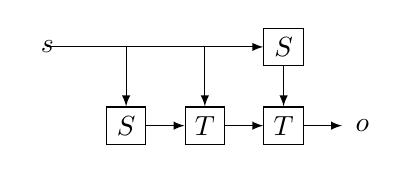
\begin{tikzpicture}[auto,>=latex,minimum width=.5cm]
  \node[] (input) {$s$};
  \node[] [right of=input] (dummy) {};
  \node[block, below of=dummy] (S1) {$S$};
  \node[block, right of=S1] (T1) {$T$};
  \node[block, right of=T1] (T2) {$T$};
  \node[block, above of=T2] (S2) {$S$};
  \node[right of=T2] (output) {$o$}; 
  \draw[->] (input) -| (S1);
  \draw[->] (input) -| (T1);
  \draw[->] (S1) -- (T1);
  \draw[->] (T1) -- (T2);
  \draw[->] (input) |- (S2);
  \draw[->] (T2) -- (output);
  \draw[->] (S2) -- (T2);
\end{tikzpicture}
\end{center}

Arrows with a single start and multiple 
ends denote a stream that is reused multiple times, e.g., $s$
in the above diagram is used 3 times.  Diagrams, however, do obscure the
ordering of the inputs of an operator; in the above examples
we have to indicate which ones are the first and respectively second inputs of $T$
if $T$ is not commutative.  Most of our binary operators are commutative.

\subsubsection{Stream operators by lifting}\label{sec:lifting}

One way of building stream operators is by (pointwise) \defined{lifting} 
functions operating on the stream values. For example, given a (scalar)
$f: A \to B$ we can define the stream operator
$\lift{f} :\stream{A} \to \stream{B}$ by $(\lift{f})(s)=f \circ s$,
or, pointwise, $(\lift{f})(s)[t] \defn f(s[t])$.

This extends straightforwardly to functions of multiple arguments, e.g.,
given $T: A \times B \rightarrow C$, we can define $\lift{T}: \stream{A} \times \stream{B}
\rightarrow \stream{C}$ as $((\lift{T})(s_0, s_1))[t] \defn T(s_0[t], s_1[t])$.
% Similarly, we omit the arrow when it is clear from the context.

We call such stream operators \defined{lifted}.
\val{I hate to be picky about this but we might want to use a different notation for 
set-theoretical pairing of elements, e.g., in functions of multiple arguments, and category-theoretical 
pairing of functions. I don't think the latter is captured properly below by $\lift\pair{.}{.}$.}

For example, applying the lifted operator $\lambda x.(2x)$ to the stream 
$\id: \N \rightarrow \N$
gives as result a stream containing all even values: \\
$(\lift{(\lambda x.(2x))})(id) = \sv{0 2 4 6 8}$.

\begin{proposition}[distributivity]\label{prop:distributivity}
Lifting distributes over function composition:
$\lift{(f \circ g)} = (\lift{f}) \circ (\lift{g})$.
\end{proposition}
\begin{proof}
This is easily proved by using associativity of function composition:
$\forall s . (\lift{(f \circ g)})(s) = (f \circ g) \circ s =
f \circ (g \circ s) = f \circ (\lift{g})(s) = (\lift{f})((\lift{g})(s)) = 
(\lift{f} \circ \lift{g})(s).$
\end{proof}

We say that two circuits are \defined{equivalent} if they compute the same
input-output function on streams.
We use the symbol $\cong$ to indicate that two circuits are 
equivalent.  For example, Proposition~\ref{prop:distributivity}
states the following circuit equivalence:

\begin{center}
\begin{tabular}{m{3.5cm}m{.3cm}m{3.5cm}}
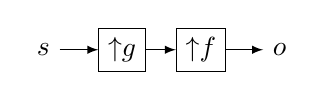
\begin{tikzpicture}[auto,>=latex]
  \node[] (input) {$s$};
  \node[block, right of=input] (g) {$\lift{g}$};
  \node[block, right of=g] (f) {$\lift{f}$};
  \node[right of=f] (output) {$o$};
  \draw[->] (input) -- (g);
  \draw[->] (g) -- (f);
  \draw[->] (f) -- (output);
\end{tikzpicture}
&
$\cong$
&
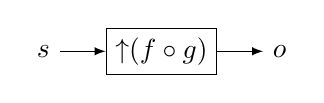
\begin{tikzpicture}[auto,>=latex]
    \node[] (input) {$s$};
    \node[block, right of=input, node distance=1.5cm] (fg) {$\lift{(f \circ g)}$};
    \node[right of=fg, node distance=1.5cm] (output) {$o$};
    \draw[->] (input) -- (fg);
    \draw[->] (fg) -- (output);
\end{tikzpicture}
\end{tabular}
\end{center}

Two (or more) streams can be combined (\textbf{paired})
into a single stream of pairs (tuples) by lifting the scalar pairing operator $\pair{\cdot}{\cdot}: A \rightarrow B \rightarrow (A \times B)$,
obtaining the stream pair operator:
$\lift{\pair{\cdot}{\cdot}}: \stream{A} \times \stream{B} \to \stream{A \times B}$,
defined as mapping $a\in\stream{A}$ and $b\in\stream{B}$ to $\pair{a}{b}\in\stream{A \times B}$
by pairing elements pointwise $\lift{\pair{a}{b}}[t] = \pair{a[t]}{b[t]} \in A \times B$.  

For example, the stream $\pair{\id}{\id}$ is the sequence of pairs \\
$\sv{\pair{0}{0} \pair{1}{1} \pair{2}{2} \pair{3}{3} \pair{4}{4}}$.

Let us also denote by $\mbox{fst}: A \times B \rightarrow A$\index{fst} 
the projection that obtains the first element of a pair $\mbox{fst}(\pair{a}{b}) = a$, 
and by $\mbox{snd}: A \times B \rightarrow B$\index{snd} the 
projection that obtains the second element of a pair. We obtain useful 
stream operators by lifting
$\lift{\mbox{fst}}$ and $\lift{\mbox{snd}}$.

\subsubsection{Basic stream operator equivalences}
\label{sec:pairing}

From type theory (or category theory) we recall the standard equalities that pairing and projections satisfy: 
$\mbox{fst}(\pair{s_0}{s_1})=s_0$, $\mbox{snd}(\pair{s_0}{s_1})=s_1$, and
$\pair{\mbox{fst}(p)}{\mbox{snd}(p)}=p$.  By lifting the functions
on both left and right we obtain some similar \textbf{equivalences of circuits}.
In some of the circuits below some inputs are not used.

\begin{center}
\begin{tabular}{m{5cm}m{.3cm}m{1.7cm}}
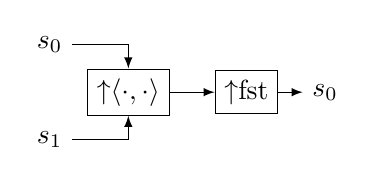
\begin{tikzpicture}[>=latex,node distance=.6cm]
  \node[] (input1) {$s_0$};
  \node[below of=input1] (midway) {};
  \node[below of=midway] (input2) {$s_1$};
  \node[block, right of=midway, node distance=1cm] (T) {$\lift{\pair{\cdot}{\cdot}}$};
  \draw[->] (input1) -| (T);
  \draw[->] (input2) -| (T);
  \node[block, right of=T, node distance=1.5cm] (F) {$\lift{\mbox{fst}}$};
  \node[right of=F, node distance=1cm] (output) {$s_0$};
  \draw[->] (T) -- (F);
  \draw[->] (F) -- (output);
\end{tikzpicture}
&
$\cong$
& 
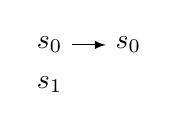
\begin{tikzpicture}[>=latex]
    \node[] (input) {$s_0$};
    \node[right of=input] (output) {$s_0$};
    \node[below of=input,node distance=.5cm] (unused) {$s_1$};
    \draw[->] (input) -- (output);
\end{tikzpicture}
\\
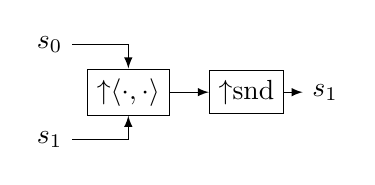
\begin{tikzpicture}[>=latex,node distance=.6cm]
  \node[] (input1) {$s_0$};
  \node[below of=input1] (midway) {};
  \node[below of=midway] (input2) {$s_1$};
  \node[block, right of=midway, node distance=1cm] (T) {$\lift{\pair{\cdot}{\cdot}}$};
  \draw[->] (input1) -| (T);
  \draw[->] (input2) -| (T);
  \node[block, right of=T, node distance=1.5cm] (F) {$\lift{\mbox{snd}}$};
  \node[right of=F, node distance=1cm] (output) {$s_1$};
  \draw[->] (T) -- (F);
  \draw[->] (F) -- (output);
\end{tikzpicture}
&
$\cong$
& 
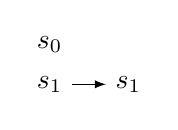
\begin{tikzpicture}[auto,>=latex]
    \node[] (input0) {$s_0$};
    \node[below of=input0,node distance=.5cm] (input1) {$s_1$};
    \node[right of=input1] (output) {$s_1$};
    \draw[->] (input1) -- (output);
\end{tikzpicture}
\\
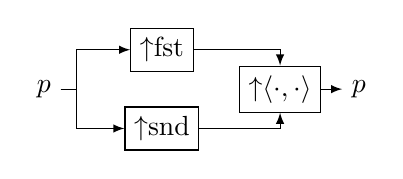
\begin{tikzpicture}[auto,>=latex]
  \node[] (input) {$p$};
  \node[right of=input, node distance=1.5cm] (midway) {};
  \node[block, above of=midway, node distance=.5cm] (fst) {$\lift{\mbox{fst}}$};
  \node[block, below of=midway, node distance=.5cm] (snd) {$\lift{\mbox{snd}}$};
  \node[block, right of=midway, node distance=1.5cm] (q) {$\lift{\pair{\cdot}{\cdot}}$};
  \node[right of=q] (output) {$p$};
  \draw[->] (input.east) -- ++(2mm,0) |- (fst);
  \draw[->] (input.east) -- ++(2mm,0) |- (snd);
  \draw[->] (fst) -| (q);
  \draw[->] (snd) -| (q);
  \draw[->] (q) -- (output);
\end{tikzpicture} 
&
$\cong$
&
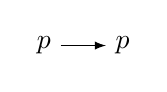
\begin{tikzpicture}[auto,>=latex]
    \node[] (input) {$p$};
    \node[right of=input] (output) {$p$};
    \draw[->] (input) -- (output);
\end{tikzpicture}
\end{tabular}
\end{center}

Pairing and projections allow for switching between pairs of streams and streams of pairs, 
whichever is more convenient. For example, instead of a binary operator 
$T:\stream{A}\times\stream{B}\to\stream{C}$ we can work with a unary operator
$T^u:\stream{A\times B}\to\stream{C}$ where $T^u(p)=T(\lift{\mbox{fst}}(p),\lift{\mbox{snd}}(p))$ 
and instead of a unary operator $Q:\stream{A\times B}\to\stream{C}$ we can work with
a binary operator $Q^b:\stream{A}\times\stream{B}\to\stream{C}$ where
$Q^b(s_0,s_1)=Q(\lift{\pair{s_0}{s_1}})$.

\begin{tabular}{m{3.5cm}m{1cm}m{5cm}}
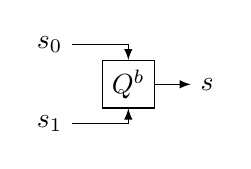
\begin{tikzpicture}[auto,>=latex]
  \node[] (input1) {$s_0$};
  \node[below of=input1,node distance=.5cm] (midway) {};
  \node[below of=midway,node distance=.5cm] (input2) {$s_1$};
  \node[block, right of=midway] (T) {$Q^b$};
  \draw[->] (input1) -| (T);
  \draw[->] (input2) -| (T);
  \node[right of=T] (output) {$s$};
  \draw[->] (T) -- (output);
\end{tikzpicture}
&
$\defn$
& 
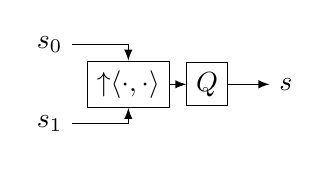
\begin{tikzpicture}[auto,>=latex]
  \node[] (input1) {$s_0$};
  \node[below of=input1,node distance=.5cm] (midway) {};
  \node[below of=midway,node distance=.5cm] (input2) {$s_1$};
  \node[block, right of=midway] (pair) {$\lift{\pair{\cdot}{\cdot}}$};
  \draw[->] (input1) -| (pair);
  \draw[->] (input2) -| (pair);
  \node[block, right of=pair] (T) {$Q$};
  \node[right of=T] (output) {$s$};
  \draw[->] (pair) -- (T);
  \draw[->] (T) -- (output);
\end{tikzpicture} \\

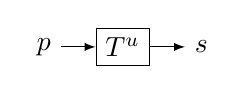
\begin{tikzpicture}[auto,>=latex]
  \node[] (input) {$p$};
  \node[block, right of=input] (Q) {$T^u$};
  \draw[->] (input) -- (Q);
  \node[right of=Q] (output) {$s$};
  \draw[->] (Q) -- (output);
\end{tikzpicture}
&
$\defn$
& 
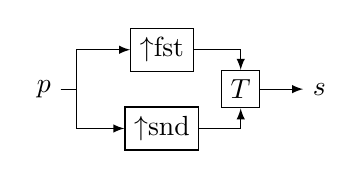
\begin{tikzpicture}[auto,>=latex]
  \node[] (input) {$p$};
  \node[right of=input, node distance=1.5cm] (midway) {};
  \node[block, above of=midway, node distance=.5cm] (fst) {$\lift{\mbox{fst}}$};
  \node[block, below of=midway, node distance=.5cm] (snd) {$\lift{\mbox{snd}}$};
  \node[block, right of=midway] (q) {$T$};
  \node[right of=q] (output) {$s$};
  \draw[->] (input.east) -- ++(2mm,0) |- (fst);
  \draw[->] (input.east) -- ++(2mm,0) |- (snd);
  \draw[->] (fst) -| (q);
  \draw[->] (snd) -| (q);
  \draw[->] (q) -- (output);
\end{tikzpicture} 
\end{tabular}


Given two operators $Q:\stream{A}\to\stream{B}$ and $R:\stream{A}\to\stream{C}$
we define $\lift{\pair{Q}{R}}:\stream{A}\to\stream{B\times C}$ by 
$\lift{\pair{Q}{R}}(s)=\lift{\pair{Q(s)}{R(s)}}$. In terms of circuit diagrams:


\begin{tabular}{m{3.5cm}m{.5cm}m{5cm}}
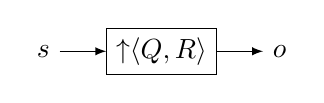
\begin{tikzpicture}[auto,>=latex]
  \node[] (input) {$s$};
  \node[block, right of=input,node distance=1.5cm] (Q) {$\lift{\pair{Q}{R}}$};
  \draw[->] (input) -- (Q);
  \node[right of=Q,node distance=1.5cm] (output) {$o$};
  \draw[->] (Q) -- (output);
\end{tikzpicture}
& 
$\cong$
&
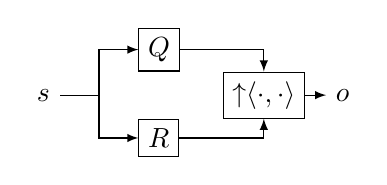
\begin{tikzpicture}[auto,>=latex,node distance=.5cm]
  \node[] (input) {$s$};
  \node[block, above right=.1cm and 1cm of input] (a) {$Q$};
  \node[block, below right=.1cm and 1cm of input] (b) {$R$};
  \node[block, right of=input, node distance=2.8cm] (P) {$\lift{\pair{\cdot}{\cdot}}$};
  \node[right of=P,node distance=1cm] (output) {$o$};
  \draw[<-] (a.west) -- ++(-5mm,0) |- (input);
  \draw[<-] (b.west) -- ++(-5mm,0) |- (input);
  \draw[->] (a) -| (P);
  \draw[->] (b) -| (P);
  \draw[->] (P) -- (output);
\end{tikzpicture}
\end{tabular}

We have standard equalities (from category theory) for this construct such
as $\lift{\mbox{fst}}\circ\lift{\pair{Q}{R}}=Q$, similarly for $\mbox{snd}$, and 
$\lift{\pair{\lift{\mbox{fst}}\circ W}{\lift{\mbox{snd}}\circ W}} = W$.
These correspond to equivalences of circuits that follow from the simpler ones above.
For example, after substituting the definition of $\pair{Q}{R}$ we have

\begin{tabular}{m{5.5cm}m{1cm}m{2.5cm}}
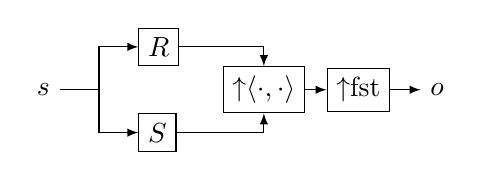
\begin{tikzpicture}[auto,>=latex,node distance=.5cm]
  \node[] (input) {$s$};
  \node[block, above right=.1cm and 1cm of input] (a) {$R$};
  \node[block, below right=.1cm and 1cm of input] (b) {$S$};
  \node[block, right of=input, node distance=2.8cm] (P) {$\lift{\pair{\cdot}{\cdot}}$};
  \node[block,right of=P,node distance=1.2cm] (F) {$\lift{\mbox{fst}}$};
  \node[right of=F,node distance=1cm] (output) {$o$};
  \draw[<-] (a.west) -- ++(-5mm,0) |- (input);
  \draw[<-] (b.west) -- ++(-5mm,0) |- (input);
  \draw[->] (a) -| (P);
  \draw[->] (b) -| (P);
  \draw[->] (P) -- (F);
  \draw[->] (F) -- (output);
\end{tikzpicture}
&
$\cong$
&
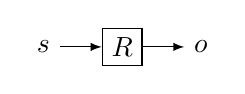
\begin{tikzpicture}[auto,>=latex]
    \node[] (input) {$s$};
    \node[block, right of=input,node distance=1cm] (F) {$R$};
    \node[right of=F] (output) {$o$};
    \draw[->] (input) -- (F);
    \draw[->] (F) -- (output);
\end{tikzpicture}
\end{tabular}


Another useful operator expression notation takes $Q:\stream{A}\to\stream{B}$
and $R:\stream{D}\to\stream{C}$ and combines them into
$Q\times R:\stream{A\times D}\to\stream{B\times C}$ where
$(Q\times R)(p) = \pair{Q(\lift{\mbox{fst}}(p))}{R(\lift{\mbox{snd}}(p))}$. 
This corresponds to the following circuit:

\begin{center}
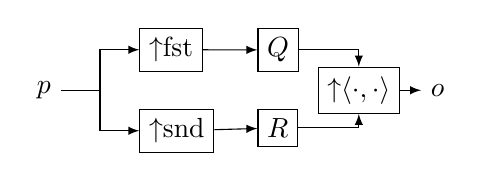
\begin{tikzpicture}[auto,>=latex,node distance=.5cm]
  \node[] (input) {$p$};
  \node[block, above right=0cm and 1cm of input] (a) {$\lift{\mbox{fst}}$};
  \node[block, above right=0cm and 2.5cm of input] (Q) {$Q$};
  \node[block, below right=0cm and 1cm of input] (b) {$\lift{\mbox{snd}}$};
  \node[block, below right=0cm and 2.5cm of input] (R) {$R$};
  \node[block, right of=input, node distance=4cm] (P) {$\lift{\pair{\cdot}{\cdot}}$};
  \node[right of=P,node distance=1cm] (output) {$o$};
  \draw[<-] (a.west) -- ++(-5mm,0) |- (input);
  \draw[<-] (b.west) -- ++(-5mm,0) |- (input);
  \draw[->] (Q) -| (P);
  \draw[->] (R) -| (P);
  \draw[->] (a) -- (Q);
  \draw[->] (b) -- (R);
  \draw[->] (P) -- (output);
\end{tikzpicture}
\end{center}

We also have the following circuit equivalence:

\begin{center}
\begin{tabular}{m{3cm}m{1cm}m{2.5cm}}
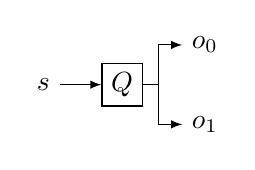
\begin{tikzpicture}[auto,>=latex]
  \node[] (input) {$s$};
  \node[block, right of=input] (q) {$Q$};
  \node[above right=0cm and .5cm of q] (a) {$o_0$};
  \node[below right=0cm and .5cm of q] (b) {$o_1$};
  \draw[->] (input) -- (q);
  \draw[->] (q.east) -- ++(2mm,0) |- (a);
  \draw[->] (q.east) -- ++(2mm,0) |- (b);
\end{tikzpicture}
&
$\cong$
&
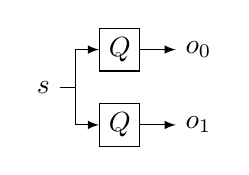
\begin{tikzpicture}[auto,>=latex]
  \node[] (input) {$s$};
  \node[block, above right=0cm and .5cm of input] (q0) {$Q$};
  \node[block, below right=0cm and .5cm of input] (q1) {$Q$};
  \node[right of=q0] (output0) {$o_0$};
  \node[right of=q1] (output1) {$o_1$};
  \draw[->] (input.east) -- ++(2mm,0) |- (q0);
  \draw[->] (input.east) -- ++(2mm,0) |- (q1);
  \draw[->] (q0) -- (output0);
  \draw[->] (q1) -- (output1);
\end{tikzpicture}
\end{tabular}
\end{center}

\val{Should this one be here? It is unrelated to products. 
Let em email you a proposal for organizing these equivalences and definitions}


Lifting functions on values and composing stream operators results in a very simple, yet limited, programming language on streams.  
We next introduce operators that ``shift'' streams in time.
These will be instrumental for enriching the language.

\subsection{Streams over abelian groups}\label{sec:abelian}

For the rest of the technical development we will require the set of values $(A, +, 0, -)$
for any stream $\stream{A}$ to form a commutative group.  

We denote by $0_{\stream{A}}$ (or simply $0$ when the type is clear) the stream that consist of the special 
value 0 at each time moment: $0_{\stream{A}} \in \stream{A}$, $\forall t \in \N . 0_{\stream{A}}[t] \defn 0_A$.

\subsubsection{Delays and time-invariance}\label{sec:delay}

\begin{definition}[Delay]
The \defined{delay operator}\footnote{The name $\zm$
comes form the DSP literature, and it is related to the z-transform.} emits an output stream that is 
the input stream delayed by one element: $\zm_A: \stream{A} \to \stream{A}$ defined by:
$$
\zm_A(s)[t] \defn  \begin{cases}
s[t - 1] & \text{when}~t\geq1\\
0_A      & \text{when}~t=0
\end{cases}
$$

We often omit the type parameter $A$, and write just $\zm$.
We denote by $z^{-k}$ the composition of $\zm$
with itself $k$ times (delay by $k$ time units). 
\end{definition}

\begin{center}
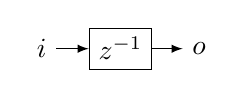
\begin{tikzpicture}[auto,node distance=1cm,>=latex]
    \node[] (input) {$i$};
    \node[block, right of=input] (z) {$\zm$};
    \node[right of=z] (output) {$o$};
    \draw[->] (input) -- (z);
    \draw[->] (z) -- (output);
\end{tikzpicture}
\end{center}

For example, the delay of the $\id$ stream is $\zm(\id)$, containing
the sequence of values $\sv{0 0 1 2 3}$.

\qquad

The following definition applies to stream operators of
any number of arguments but to keep the notation simpler we formulate it only for binary operators.

\begin{definition}[Time invariance]
A stream operator $T: \stream{A_0}\times\stream{A_1} \to \stream{B}$ is \defined{time-invariant} if it commutes with the delay operator $\zm$, that is, \\
$T(\zm(s_0),\zm(s_1)) = \zm(T(s_0,s_1))$ for any $s_0 \in \stream{A_0}, s_1 \in \stream{A_1}$.
\end{definition}
In other words, $T$ is time-invariant if and only if the following two circuits are equivalent:

\begin{center}
\begin{tabular}{m{3cm}m{.5cm}m{3cm}}
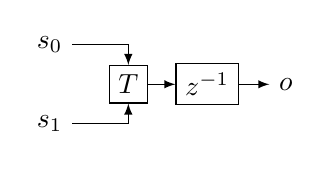
\begin{tikzpicture}[auto,node distance=.5cm,>=latex]
  \node[] (input1) {$s_0$};
  \node[below of=input1] (midway) {};
  \node[below of=midway] (input2) {$s_1$};
  \node[block, right of=midway, node distance=1cm] (T) {$T$};
  \node[block, right of=T,node distance=1cm] (z) {$\zm$};
  \node[right of=z,node distance=1cm] (output) {$o$};
  \draw[->] (input1) -| (T);
  \draw[->] (input2) -| (T);
  \draw[->] (T) -- (z);
  \draw[->] (z) -- (output);
\end{tikzpicture}
&
$\cong$
&
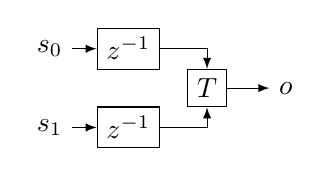
\begin{tikzpicture}[auto,node distance=.5cm,>=latex]
  \node[] (input1) {$s_0$};
  \node[below of=input1] (midway) {};
  \node[below of=midway] (input2) {$s_1$};
  \node[block, right of=input1, node distance=1cm] (z1) {$\zm$};
  \node[block, right of=input2, node distance=1cm] (z2) {$\zm$};
  \node[block, right of=midway, node distance=2cm] (T) {$T$};
  \node[right of=T,node distance=1cm] (output) {$o$};
  \draw[->] (input1) -- (z1);
  \draw[->] (input2) -- (z2);
  \draw[->] (z1) -| (T);
  \draw[->] (z2) -| (T);
  \draw[->] (T) -- (output);
\end{tikzpicture}
\end{tabular}
\end{center}

It is straightforward to check that the composition
of any number of time-invariant operators of any number of arguments
is time invariant. Similarly, the delay operators $z^{-k}$ as well as the
pairing and projection operators are time-invariant. 
In this framework we only deal with time-invariant operators.

\begin{definition}
We say that a function between groups $f: A \to B$ has the \defined{zero-preservation
property} iff $f(0_A) = 0_B$.  We write $\zpp{f}$.  This property generalizes to functions
with multiple inputs: e.g., $g: A \times B \to C$ where $A, B, C$ are groups.  $\zpp{g}$ 
iff $g(0_A, 0_B) = 0_C$.
\end{definition}

\begin{proposition}
A lifted operator $\lift{f}$ is time-invariant iff $\zpp{f}$. 
\end{proposition}

Notice that it is easy to construct operators that are not time-invariant.
Consider the ``constant 1'' function: $c_1: \N \rightarrow \N$, defined by 
$c_1(x) = 1, \forall x \in \N$.
The stream operator defined by $\lift{c_1}: \stream{N} \rightarrow \stream{N}$ 
produces a stream containing only the constant value 1: $c_1(s)[t] = 1, 
\forall s \in \stream{N}, t \in \N$.  The stream operator $\lift{c_1}$
is \emph{not} time-invariant, since it does not have the zero preservation property.

\begin{comment}
\begin{definition}
We call an operator $o: \stream{A} \rightarrow \stream{B}$ over streams 
\defined{memoryless} if it can be produced by lifting a function pointwise, i.e., 
there exists a function $f: A \rightarrow B$ such that 
$\forall s \in \stream{A} . o(s)[t] = f(s[t])$.

\begin{example}
Whatever definition we give to ``memoryless'' it should be the case that 
any memoryless operator is causal. 
\end{example}
\end{definition}
\end{comment}

\subsection{Causal and strict operators}\label{sec:causal}

For notation simplicity we again give the next definition only for unary operators;
it extends naturally to binary operators through the use of pairing as shown above.

\begin{definition}[Causality]
A stream operator, $S:\stream{A}\to\stream{B}$,
is \defined{causal} when for any $s,s'\in\stream{A}$,
and all times $t$ we have 
$$
(\forall i\leq t~s[i]=s'[i]) ~~\text{implies}~~ S(s)[t]=S(s')[t]
$$
\end{definition}

Note that all operators produced by lifting scalar functions are causal. 
$\zm$ is causal.  All \dbsp operators are causal.

\begin{definition}[Cutting]
\defined{Cutting} the stream $s \in \stream{A}$ at time $t \in \N$ produces a stream
$$
(\cut{s}{t})[i] \defn  \begin{cases}
                      s[i] &\text{if}~i\leq t\\
                      0_A  &\text{if}~i>t
                      \end{cases}
$$
\end{definition}
For example, cutting the stream $\id$ at time 2 gives the stream $\cut{\id}{2}$
composed of the sequence $\sv{0 1 2 0 0}$.

Note that $\cut{\cut{s}{t_1}}{t_2}=\cut{s}{\min(t_1,t_2)}$. It follows that
$\cut{\cut{s}{t_1}}{t_2}=\cut{\cut{s}{t_2}}{t_1}$ (cutting is commutative) and
$\cut{\cut{s}{t}}{t}=\cut{s}{t}$, (cutting at time $t$ is idempotent).
Cutting, however, is \textbf{not} time-invariant.  Cutting is not 
used as a \dbsp operator, it is just a mathematical tool that we will use to 
reason about the behavior of the circuits we build.

\begin{lemma}
\label{lemma-causal-characterization}
The following are equivalent for a binary stream operator $T$
\begin{enumerate}
\item[(i)] $T$ is causal
\item[(ii)] $\forall s_1,s_2$ and $t$  we have $\cut{T(s_1,s_2)}{t} ~=~ \cut{T(\cut{s_1}{t},\cut{s_2}{t})}{t}$~.
\end{enumerate}
\end{lemma}
Using part (ii) it follows immediately that the composition
of any number of causal operators of any number of arguments is causal.
Moreover, using also the commutativity and idempotence of cutting, it follows that
for any $t$ the operator $\lambda s.\cut{s}{t}$ is itself causal.

\begin{definition}[zero almost everywhere]\label{def:zae}
We say that a stream $s$ is \defined{zero almost-everywhere} if there exists a time $t_0 \in \N$
s.t. $\cut{s}{t_0} = s$.
\end{definition}

%Such a stream can be described entirely by providing its prefix up to time $t_0$,
%a finite stream.  
We denote the set of streams over $A$ that are zero almost everywhere
by $\streamf{A}$.

\begin{definition}[Strictness]
A stream operator, $F:\stream{A}\to\stream{B}$
is \defined{strictly causal} (abbreviated \textbf{strict})
if for any $s,s'\in\stream{A}$ and all times $t$ we have 
$$
(\forall i<t . s[i]=s'[i]) ~~\text{implies}~~ F(s)[t]=F(s')[t]
$$
\end{definition}

In particular, $F(s)[0] = 0_B$ is the same for all inputs $s \in \stream{A}$.
Strict operators are of course causal. Note that lifted stream operators,
while causal, in general are \emph{not} strict. 

It can be immediately checked that the operator $\zm$ 
(in fact, $z^{-k}$ for any positive integer $k$)  
is strict. 
In this text $\zm$ is the only primitive strict operator used.

\begin{definition}[Strict cutting]
\defined{Strictly cutting} the stream $s \in \stream{A}$ at time $t \in \N$ produces the stream
$$
(\scut{s}{t})[i] \defn  \begin{cases}
                      s[i] &\text{if}~i< t\\
                      0_A  &\text{if}~i\geq t
                      \end{cases}
$$
\end{definition}

$\scut{s}{0}$ is the stream $0_{\stream{A}}$ that is $0_A$ at all times.
Note also that $\scut{s}{t+1} =\cut{s}{t}$.


Analogously to Lemma~\ref{lemma-causal-characterization} an operator $F: \stream{A} \to \stream{B}$ is strict iff for any $s$ and $t$ we have
$$
\cut{F(s)}{t} ~=~ \cut{F(\scut{s}{t})}{t}
$$
In particular, $F(s)[0] = F(0_{\stream{A}})[0]$ and
$F(s)[t+1]=F(\cut{s}{t})[t+1]$.  Note the different zeros in $F(0_{\stream{A}})[0]$: 
it features both the stream $0_{\stream{A}} \in \stream{A}$, consisting of the group element $0_A$ 
at each time moment, and the time moment $0$.

The next proposition shows the importance of strict operators.
\begin{proposition}
\label{prop-unique-fix}
For any strict operator $F: \stream{A} \to \stream{A}$ the equation ~$\alpha=F(\alpha)$~ has a unique
solution $\alpha \in \stream{A}$.  In other words, every strict operator has a unique fixed point,
which we denote by $\fix{\alpha}{F(\alpha)}$.
\end{proposition}
%\leonid{Usually fixed-points require some monotonicity.  What is it here?}

\begin{proof}
Define the solution (the fixed point) by recurrence:
\begin{eqnarray*}
\alpha[0] & = &  F(\alpha)[0]=F(0_{\stream{A}})[0]\\
\alpha[t+1] & = & F(\alpha)[t+1]=F(\cut{\alpha}{t})[t+1]
\end{eqnarray*}
The second equality defines $\alpha[t+1]$ in terms of $\alpha[0],\ldots,\alpha[t]$.
Uniqueness follows by strong induction.

\qquad
\end{proof}

We will apply the previous proposition to operators obtained by composing strict and causal ones.
\begin{lemma} 
\label{lemma-causal-strict}
Let $k\geq 2$. If $F$ is strict and the $k$-ary $T$ operator is causal, then for any 
fixed $s_0,\ldots,s_{k-2}$ the operator
$\lambda\alpha.T(s_0,\ldots,s_{k-2},F(\alpha))$ is strict. 
\end{lemma}

\begin{proof} We show the case $k=2$.
This operator is described by the following diagram with a ``feedback loop'':

\begin{center}
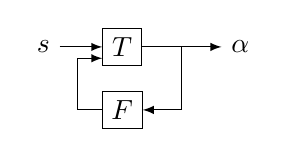
\begin{tikzpicture}[>=latex]
    \node[] (input) {$s$};
    \node[block, right of=input] (f) {$T$};
    \node[right of=f, node distance=1.5cm] (output) {$\alpha$};
    \node[block, below of=f, node distance=.8cm] (z) {$F$};
    \draw[->] (input) -- (f);
    \draw[->] (f) -- node (mid) {} (output);
    \draw[->] (mid.center) |-  (z);
    \draw[->] (z.west) -- ++(-.3,0) |- ([yshift=1mm]f.south west);
\end{tikzpicture}
\end{center}
\begin{eqnarray*}
\cut{T(s,F(\alpha))}{t} & = & \cut{T(\cut{s}{t},\cut{F(\alpha)}{t})}{t}\\
                   & = & \cut{T(\cut{s}{t},\cut{F(\scut{\alpha}{t})}{t})}{t}\\
                   & = & \cut{T(s,F(\scut{\alpha}{t}))}{t}
\end{eqnarray*}
\qquad
\end{proof}


\begin{corollary} 
\label{cor-fix-cut}
For strict $F$ we have
$$
\cut{(\fix{\alpha}{F(\alpha)})}{t} ~=~  \fix{\alpha}{(\cut{F(\alpha)}{t})}
$$
\end{corollary}
\begin{proof}
Since cutting itself is a causal operator, it follows from Lemma~\ref{lemma-causal-strict} that $\lambda\alpha.(\cut{F(\alpha)}{t})$ is strict
so Proposition~\ref{prop-unique-fix} applies and $\fix{\alpha}{(\cut{F(\alpha)}{t})}$
is well-defined.

If we let $\alpha$ be the solution of $\alpha=F(\alpha)$ then, by uniqueness, it suffices to show that $\beta=\cut{\alpha}{t}$ satisfies 
the equation $\beta=\cut{F(\beta)}{t}$. Indeed, since $F$ is in particular causal
$$
\cut{\alpha}{t} = \cut{F(\alpha)}{t} = \cut{F(\cut{\alpha}{t})}{t}
$$


\qquad
\end{proof}

\begin{corollary}\label{feedback-semantics}
\label{cor-loop}
Let $k\geq1$. If $F: \stream{A} \to \stream{A}$ is strict and $(k+1)$-ary $T$ is causal then the $k$-ary
operator $Q(s_0,\ldots,s_{k-1})=\fix{\alpha}{T(s_0,\ldots,s_{k-1},F(\alpha))}$~ is well-defined and causal. 
If, moreover, $F$ and $T$ are time-invariant then so is $Q$.
\end{corollary}
\begin{proof} We show the case $k=1$.
The well-definedness of $Q$ follows by applying, for each $s$, Proposition~\ref{prop-unique-fix}
to the operator
$\lambda\alpha.T(s,F(\alpha))$ which is strict by Lemma~\ref{lemma-causal-strict}.
For future reference it might be useful to state the defining recurrence for a stream $\alpha$ 
produced by this operator, that is, $\alpha=Q(s)$:
\begin{eqnarray*}
\alpha[0] & = &  T(s,F(0_{\stream{A}}))[0]\\
\alpha[t+1] & = & T(s,F(\cut{\alpha}{t}))[t+1]
\end{eqnarray*}
To prove that $Q$ is causal we could use this recurrence and induction. Instead 
we use the causality of $T$ and the idempotence of cutting in conjunction with
Corollary~\ref{cor-fix-cut} as follows:
\begin{eqnarray*}
\cut{Q(s)}{t} & = &  \cut{(\fix{\alpha}{T(s,F(\alpha))})}{t}\\
         & = &  \fix{\alpha}{\cut{(T(s,F(\alpha))}{t})}~~~~~~~~~~~~\mbox{(Corollary~\ref{cor-fix-cut})}\\
         & = &  \fix{\alpha}{(\cut{T(\cut{s}{t},\cut{F(\alpha)}{t})}{t})}~~~~~~\mbox{(Causality of $T$)}\\
         & = &  \fix{\alpha}{(\cut{T(\cut{\cut{s}{t}}{t},\cut{F(\alpha)}{t})}{t})}~~~\mbox{(Idempotence of cutting)}\\
         & = &  \fix{\alpha}{\cut{(T(\cut{s}{t},F(\alpha))}{t})}~~~~~~~~~~\mbox{(Causality of $T$)}\\
         & = & \cut{(\fix{\alpha}{T(\cut{s}{t},F(\alpha))})}{t}~~~~~~~~~~\mbox{(Corollary~\ref{cor-fix-cut})}\\
         & = & \cut{Q(\cut{s}{t})}{t}
\end{eqnarray*}
For time-invariance we observe that if $\alpha=T(s,F(\alpha))$ then $\zm(\alpha)= \zm(T(s,F(\alpha)))=T(\zm(s),\zm(F(\alpha))= 
T(\zm(s),F(\zm(\alpha)))$. It follows that $\beta=\zm(\alpha)$ satisfies the equation $\beta=T(\zm(s),F(\beta))$ so, 
by uniqueness of the fixed point $Q(\zm(s))=\zm(Q(s))$.
\end{proof}



Ostensibly this covers a form of straightforward recursion but how about mutual recursion? For instance, assuming $T_1,T_2$ are causal and $F_1,F_2$ are strict we wish to claim that the following is well defined: $Q_1(s_1,s_2)=\alpha_1$ and $Q_2(s_1,s_2)=\alpha_2$ where:
\begin{eqnarray*}
\alpha_1 & = & T_1(s_1,F_1(\alpha_2))~~~~~\mbox{and}\\
\alpha_2 & = & T_2(s_2,F_2(\alpha_1))
\end{eqnarray*}
Here is the corresponding diagram:

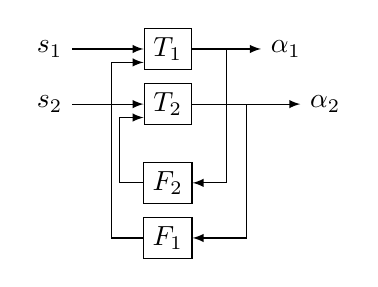
\begin{tikzpicture}[>=latex]
  \node[] (i1) {$s_1$};
  \node[below of=i1, node distance=.7cm] (i2) {$s_2$};
  \node[block, right of=i1, node distance=1.5cm] (t1) {$T_1$};
  \node[block, right of=i2, node distance=1.5cm] (t2) {$T_2$};
  \node[right of=t1, node distance=1.5cm] (o1) {$\alpha_1$};
  \node[right of=t2, node distance=2cm] (o2) {$\alpha_2$};
  
  \node[block, below of=t2] (f1) {$F_2$};
  \node[block, below of=f1, node distance=.7cm] (f2) {$F_1$};
  
  \draw[->] (i1) -- (t1);
  \draw[->] (i2) -- (t2);
  \draw[->] (t1) -- node (m1) {} (o1);
  \draw[->] (t2) -- node (m2) {} (o2);
  \draw[->] (m1.center) |- (f1);
  \draw[->] (m2.center) |- (f2);
  
  \draw[->] (f1.west) -- ++(-.3,0) |- ([yshift=1mm]t2.south west);
  \draw[->] (f2.west) -- ++(-.4,0) |- ([yshift=1mm]t1.south west);
  
\end{tikzpicture}

In section~\ref{sec:pairing} we defined constructions on pairs of streams/streams of pairs. 
%that we defined in Section~\ref{sec:cartesian} 
In particular, for binary $T_1:\stream{A_1}\times\stream{B_1}\to\stream{C_1}$ and 
binary $T_2:\stream{A_2}\times\stream{B_2}\to\stream{C_2}$ 
let
\val{For binary operators we should have defined $\times$ this way in section~\ref{sec:pairing} ...
Also, in the def of $T_1\times T_2$ note that I did not put a lift in front of the stream pairing operator on the RHS. }
binary $T_1\times T_2:\stream{A_1\times A_2}\times\stream{B_1\times B_2}\to\stream{C_1\times C_2}$ 
$$
[T_1\times T_2](p,q) = \pair{T_1(\lift{\mbox{fst}}\circ p,\lift{\mbox{fst}}\circ q)}
{T_2(\lift{\mbox{snd}}\circ p,\lift{\mbox{snd}}\circ q)}
$$
In addition, we use $F_1\times F_2:\stream{C_1\times C_2}\to\stream{B_1\times B_2}$ as defined in section~\ref{sec:pairing}. Let also $\mbox{swap}: C_1\times C_2 \to C_2 \times C_1$
be the operator that swaps the components of a pairs (obtained by pairing the second projection
with the third.
\begin{proposition}
If $T_1$ and $T_2$ are causal then $T_1\circ T_2$ is causal. If $F_1$ and $F_2$ are strict then
$(F_1\times F_2)\circ\lift{\mbox{swap}}$ is strict.
\end{proposition}
The circuit above is equivalent to the following (when composed with projections of outputs
and pairing of inputs:

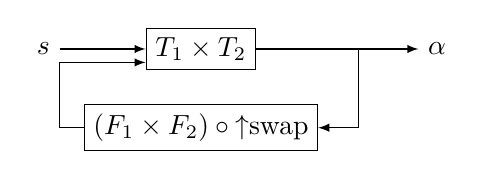
\begin{tikzpicture}[>=latex]
    \node[] (input) {$s$};
    \node[block, right of=input, node distance=2cm] (f) {$T_1\times T_2$};
    \node[right of=f, node distance=3cm] (output) {$\alpha$};
    \node[block, below of=f] (z) {($F_1\times F_2)\circ\lift{\mbox{swap}}$};
    \draw[->] (input) -- (f);
    \draw[->] (f) -- ++(2,0) node (mid) {} -- (output);
    \draw[->] (mid.center) |-  (z);
    \draw[->] (z.west) -- ++(-.3,0) |- ([yshift=1mm]f.south west);
\end{tikzpicture}


In other words, 
we can apply Corollary~\ref{feedback-semantics} to the causal operator $T_1\times T_2$
and the strict operator $F_1\times F_2$ and obtain $Q_1$ and $Q_2$ from
$$
\fix{\alpha}{[T_1\times T_2](\pair{s_1}{s_2},[F_1\times F_2](\mbox{swap}(\alpha)))}
$$
by further projecting, where $\alpha$ is a variable of type pair of streams and $\overline{\alpha}$
swaps the two components.





\val{We should state this a some kind of corollary to the corollary.}
\mihai{This becomes complicated for $n$-way mutual recursion, you have a quadratic number of edges.
Maybe it's simpler to assume that all of them use all of the alphas, and the projection to a subset
is part of $T$ if needed.}



\subsection{Streams as an abelian group}\label{sec:abelianstreams}

Remember that we require the elements of a stream to come from an Abelian group:
$(A,+,0,-)$.  This structure also lifts to streams:

\begin{proposition}
$(\stream{A},+,0_{\stream{A}},-)$ (with the operations lifted pointwise in time) 
is also an abelian group. Moreover, lifting a group homomorphism produces
a stream operator that is itself a group homomorphism.
In addition, when $A$ and $B$ are abelian groups there is a standard abelian group structure
on $A\times B$, with the zero $0_{A \times B}$ the pair $\pair{0_A}{0_B}$.
\end{proposition}


\begin{definition}[linear]
If $A$ and $B$ are abelian groups, we call
a function $f: A \rightarrow B$ \defined{linear} if it is a group homomorphism, that is,
$f(a+b)=f(a)+f(b)$ (and therefore $f(0_A)=0_B$ and $f(-a)=-f(a)$); thus $\zpp{f}$.
\end{definition}

We use the abbreviation LTI for a stream operator that is linear and time-invariant.

Lifting a linear function $f: A \to B$ produces a stream operator $\lift{f}$ that is causal and LTI. 
It follows that stream addition and negation are causal and LTI.
$\zm$ is LTI, (and so is $z^{-k}$ for all $k$).

\begin{definition}[multilinear, bilinear]
We define \defined{multilinear} (in particular, \defined{bilinear}) functions as functions (between groups) of multiple
arguments that are linear separately in each argument (that is, if we fix all but one argument,
the resulting function is linear in that argument.  In other words, the function distributes over addition): 
e.g., for $g: A_0 \times A_1 \to B, \forall a, b \in A_0, c, d \in A_1 . g(a+b, c) = g(a, c) + g(b, c)$, 
and $g(a, c+d) = g(a, c) + g(c, d)$.
\end{definition}

Multiplication over $\Z$ is a bilinear function.  For a bilinear function $g$ we have $\zpp{g}$.

This definition extends to stream operators.
Lifting any bilinear function $g: A \times B \to C$ produces a bilinear stream operator $\lift{g}$.
An example bi-linear operator over $\stream{\Z}$ is the lifted integer multiplication: 
$T: \stream{\Z} \times \stream{\Z} \to \stream{\Z}, T(a, b)[t] = a[t]\cdot b[t]$.

The composition of multilinear operators with linear operators is multilinear (since homomorphisms compose).
Since linear and bilinear functions have the zero-preservation property,
lifted linear and bilinear functions operators are all time-invariant.

\begin{proposition}
The composition of a bilinear operator followed by a linear operator is a bilinear operator.
\end{proposition}
\begin{proof}
Consider $T: \stream{A} \times \stream{B} \to \stream{C}$ a bilinear operator, and 
$S: \stream{C} \to \stream{C}$, a linear operator.  Let us compute $S(T(a+b, c)) = S(T(a, c) + T(b, c)) = 
S(T(a, c)) + S(T(b, c)).$  Thus $S \circ T$ is bilinear.
\end{proof}

Lifting a multilinear operator $A_1\times\cdots\times A_n \rightarrow B$ produces a multilinear, time-invariant stream operator. Although combining pairs (tuples) of 
streams into stream of pairs (tuples) can be useful
we must note a distinction (well understood in algebra): 
we have seen that we can use instead of a binary stream operator
$T:\stream{A}\times\stream{B}\to\stream{C}$ a unary version that acts on streams of pairs
$T^u:\stream{A\times B}\to\stream{C}$ where $T^u\pair{a}{b}=T(a,b)$. However, in contrast to causality,
there is, in general, no relation between the linearity. %\footnote{Recall the
%abelian group structure on $A\times B$.} of $T^u$ and the bilinearity of $T$. 
%\mihai{I still think that the motivation for this statement is unclear.}

In traditional signal processing most operators are LTI but in our development
we will use some important non-linear ones. 

The ``feedback-loop'' operators defined by recurrence in Corollary~\ref{cor-loop},
e.g., $\lambda s.\fix{\alpha}{T(s,F(\alpha))}$ are, in general, not (multi)linear.
\val{Counterexample even for bilinear $S$ and $\lambda s_1.\lambda s_2.\fix{\alpha}{S(s_1,s_2+\zm(\alpha))}$? Possibly $S$ is join NOT followed by distinct?}
However, multilinearity holds in important particular cases,
as shown in the following proposition:

\begin{proposition}
\label{prop-rec-linear}
Let $S$ be a unary causal, LTI operator. Then, the
operator $Q(s)=\fix{\alpha}{S(s+\zm(\alpha))}$~ is well-defined and LTI.
\end{proposition}
\mihai{Notice that this is a very nice kind of recursion, a tail-recursion.}

\begin{center}
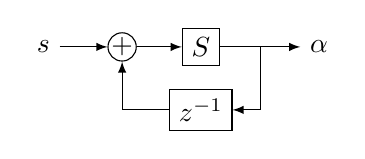
\begin{tikzpicture}[>=latex]
    \node[] (input) {$s$};
    \node[block, shape=circle, right of=input, inner sep=0pt] (plus) {$+$};
    \node[block, right of=plus] (Q) {$S$};
    \node[right of=Q, node distance=1.5cm] (output) {$\alpha$};
    \node[block, below of=Q, node distance=.8cm] (z) {$\zm$};
    \draw[->] (input) -- (plus);
    \draw[->] (plus) -- (Q);
    \draw[->] (Q) -- node (mid) {} (output);
    \draw[->] (mid.center) |-  (z);
    \draw[->] (z) -| (plus);
\end{tikzpicture}
\end{center}

\begin{proof} Since $S$ and the addition operator
are causal and $\zm$ is strict, Proposition~\ref{prop-unique-fix} applies, 
for each $s$, to the operator
$\lambda\alpha.S(s+\zm(\alpha))$ which is strict by Lemma~\ref{lemma-causal-strict}.
Thus $Q$ is well-defined.

Fix streams $s_0$ and $s_1$. Let $\alpha_0$
be the unique solution of $\alpha_0=S(s_0+\zm(\alpha_0))$ and 
$\alpha_1$ be the unique solution of $\alpha_1=S(s_1+\zm(\alpha_1))$.
Then $\alpha=\alpha_0+\alpha_1$ is the unique solution of 
$\alpha=Q(s_0+s_1+\zm(\alpha))$. This is justified by adding the equations
and using the linearity of $S$ and the linearity of $\zm$.
\end{proof}

\begin{proposition}
If $T$ is binary causal, $G$ is unary causal, and $F$ is unary strict then:
$$
\fix{\alpha}{G(T(s,F(\alpha)))} = G(\fix{\beta}{T(s,F(G(\beta)))})
$$

\noindent In terms of diagrams:

\begin{tabular}{m{4cm}m{1cm}m{5cm}}
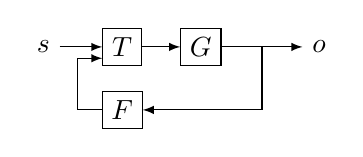
\begin{tikzpicture}[>=latex]
    \node[] (input) {$s$};
    \node[block, right of=input] (t) {$T$};
    \node[block, right of=t] (g) {$G$};
    \node[right of=g, node distance=1.5cm] (output) {$o$};
    \node[block, below of=t, node distance=.8cm] (f) {$F$};
    \draw[->] (input) -- (t);
    \draw[->] (t) -- (g);
    \draw[->] (g) -- node (mid) {} (output);
    \draw[->] (mid.center) |-  (f);
    \draw[->] (f.west) -- ++(-.3,0) |- ([yshift=1mm]t.south west);
\end{tikzpicture}
&
$\cong$
&
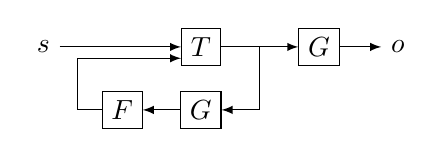
\begin{tikzpicture}[>=latex]
    \node[] (input) {$s$};
    \node[block, right of=input, node distance=2cm] (t) {$T$};
    \node[block, right of=t, node distance=1.5cm] (g) {$G$};
    \node[right of=g] (output) {$o$};
    \node[block, below of=t, node distance=.8cm] (g1) {$G$};
    \node[block, left of=g1] (f) {$F$};
    \draw[->] (input) -- (t);
    \draw[->] (t) -- node (mid) {} (g);
    \draw[->] (g) -- (output);
    \draw[->] (mid.center) |-  (g1);
    \draw[->] (g1) -- (f);
    \draw[->] (f.west) -- ++(-.3,0) |- ([yshift=1mm]t.south west);
\end{tikzpicture}
\end{tabular}
\end{proposition}

\begin{proof}
For the second fixpoint to exist we need to show that $F\circ G$ is strict.
Once we do that, by uniqueness of solutions, it remains to show that if $\beta$ is a solution to  $\beta=T(s,F(G(\beta))$ then $\alpha=G(\beta)$ is a solution to
$\alpha=G(T(s,F(\alpha))$ which is immediate by applying $G$ to the first equation.
So let's prove that $F\circ G$ is strict. For $t>0$ we have
\begin{eqnarray*}
\cut{F(G(s))}{t} & = & \cut{F(\scut{G(s)}{t})}{t}~~~~~\mbox{($F$ strict)}\\
                 & = & \cut{F(\cut{G(s)}{t-1})}{t}~~~~~\mbox{($t\geq1$)}\\
                 & = & \cut{F(G(\cut{s}{t-1}))}{t}~~~~~\mbox{($G$ causal)}\\ 
                 & = & \cut{F(G(\scut{s}{t}))}{t}
\end{eqnarray*}
For $t=0$ just observe that $F(G(s))[0]$ is the same for any $G(s)$ therefore for any $s$.
Note that if $G$ is not causal then $F\circ G$ is not strict and the fixed point may not exist.
\end{proof}


\subsection{Differentiation and Integration}

\begin{definition}[Differentiation]
The \defined{differentiation operator} $\D_{\stream{A}} : \stream{A} \to \stream{A}$ is defined by:
$$
\D_{\stream{A}}(s) \defn s - \zm(s)
$$ 
\end{definition}
We generally omit the type, and write just $\D$ when the type can be inferred from the context.

The value of $\D(s)$ (at time $t$) is the difference
between  the current (time $t$) value of $s$ and the previous (time $t-1$) value of $s$.

As an example, applying $\D$ to the stream $\id$ gives a result a
stream $\D(\id)$ containing the values $\sv{0 1 1 1 1}$.

\begin{center}
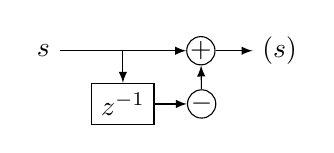
\begin{tikzpicture}[auto,>=latex,node distance=1cm]
    \node[] (input) {$s$};
    \node[block, shape=circle, right of=input, inner sep=0pt,node distance=2cm] (plus) {$+$};
    \node[right of=plus] (output) {$\D(s)$};
    \draw[draw,->] (input) -- node (i) {} (plus);
    \node[block, below of=i, node distance=.8cm] (z) {$\zm$};
    \node[block, shape=circle, right of=z, inner sep=0pt] (minus) {$-$};
    \draw[->] (plus) -- (output);
    \draw[->] (i) -- (z);
    \draw[->] (z) -- (minus);
    \draw[->] (minus) -- (plus);
\end{tikzpicture}
\end{center}

\begin{proposition}
\label{prop-diff-properties}
The differentiation operator $\D$ is causal and LTI.
\end{proposition}
\begin{proof}
Follow from definition using the properties of subtraction and delay.
\end{proof}

The integration operator ``reconstitutes'' a stream from its changes:

\begin{definition}[Integration]
The \defined{integration operator}  $\I_{\stream{A}} : \stream{A} \to \stream{A}$ 
is defined by $\I_{\stream{A}}(s) \defn \lambda s . \fix{\alpha}{(s + \zm(\alpha))}$.
\end{definition}

\noindent
We also generally omit the type, and write just $\I$.
This is the construction from Proposition~\ref{prop-rec-linear} 
using the identity function for $S$.

\begin{center}
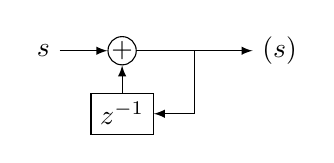
\begin{tikzpicture}[auto,>=latex]
    \node[] (input) {$s$};
    \node[block, shape=circle, right of=input, inner sep=0pt] (plus) {$+$};
    \node[right of=plus, node distance=2cm] (output) {$\I(s)$};
    \node[block, below of=plus, node distance=.8cm] (z) {$z^{-1}$};
    \draw[draw,->] (input) -- (plus);
    \draw[->] (plus) -- node (o) {} (output);
    \draw[->] (o) |- (z);
    \draw[->] (z) -- (plus);
\end{tikzpicture}
\end{center}

As an example, applying $\I$ to the $\id$ stream gives as result
a stream $\I(\id)$ composed of the values $\sv{0 1 3 6 10}$.

\begin{proposition}~\label{iprop}
$\I(s)$ is the discrete (indefinite) integral applied to the stream $s$: 
$\I(s)[t] = \sum_{i \leq t} s[i]$.
\end{proposition}
\begin{proof} The recurrence from Corollary~\ref{cor-loop} specializes to
\begin{eqnarray*}
\alpha[0]  & = & s[0]\\
\alpha[t+1] & = & \alpha[t] + s[t+1]
\end{eqnarray*}
and it's straightforward to check that $\alpha[t]= \sum_{i \leq t} s[i]$ satisfies 
it.
\end{proof}

\begin{proposition}[Properties of $\I$] 
\label{prop-integ-properties}
The integration operator $\I$ is causal and LTI.
\end{proposition}
\begin{proof}
By Proposition~\ref{iprop} these properties follow from Corollary~\ref{cor-loop} and Proposition~\ref{prop-rec-linear}.  They also be checked directly using
the definition by summation.
\end{proof}


\begin{theorem}[Inversion]
\label{inverses}
The integration and differentiation operators are inverse to each other. Equivalently, for any streams 
$\alpha$ and $s$ we have $\alpha=\I(s)$ iff $\D(\alpha)=s$.
\end{theorem}
\begin{proof}
This can be shown directly from the definitions, for example
  $$
  \begin{aligned}
  \D(\I(s))[t] &= (\I(s) - \zm(\I(s)))[t] & \mbox{definition of }\D \\
  &= \sum_{k \leq t} s[k] - \zm(\sum_{k \leq t} s[k])[t] &
  \mbox{Property }~\ref{prop-integ-properties} \\
  &= \sum_{k \leq t} s[k] - \sum_{k \leq t-1} s[k] & \mbox{definition of }\zm \\
  &= s[t]
  \end{aligned}
  $$
(and similarly we can show that $\I(\D(s'))[t] =s'[t]$).
  
Alternatively, the equivalent form of the theorem follows from Proposition~\ref{iprop} by observing that
$\D(\alpha)=s$ iff $\alpha=s+\zm(\alpha)$ which is the equation on streams that defines $\alpha=\I(s)$.
%A third proof, bringing some new insights, is given in Section~\ref{sec:ztransform}.
\end{proof}

So we have the following circuit equivalence:

\noindent
\begin{tabular}{m{3.5cm}m{.7cm}m{1.5cm}m{.7cm}m{3.5cm}}
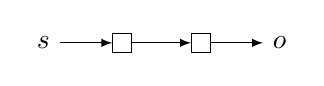
\begin{tikzpicture}[auto,>=latex]
    \node[] (input) {$s$};
    \node[block, right of=input] (I) {$\I$};
    \node[block, right of=I] (D) {$\D$};
    \node[right of=D] (output) {$o$};
    \draw[->] (input) -- (I);
    \draw[->] (I) -- (D);
    \draw[->] (D) -- (output);
\end{tikzpicture}
     &  
     $\cong$
     &
\begin{tikzpicture}[auto,>=latex]
    \node[] (input) {$s$};
    \node[right of=input] (output) {$o$};
    \draw[->] (input) -- (output);
\end{tikzpicture}
     &
     $\cong$
     &
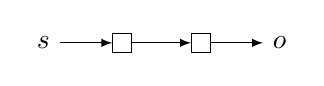
\begin{tikzpicture}[auto,>=latex]
    \node[] (input) {$s$};
    \node[block, right of=input] (D) {$\D$};
    \node[block, right of=D] (I) {$\I$};
    \node[right of=I] (output) {$o$};
    \draw[->] (input) -- (D);
    \draw[->] (D) -- (I);
    \draw[->] (I) -- (output);
\end{tikzpicture}
\end{tabular}


Since $\I$ and $\D$ are inverse to each other they are both bijections on streams.

If we define addition of pairs as adding the pair elements pointwise, we also have
the following identities: $\I(\pair{s}{t}) = \pair{\I(s)}{\I(t)}$ and $\D(\pair{s}{t}) = \pair{\D(s)}{\D(t)}$.

\paragraph{Observation}
It is a standard algebraic fact that the inverse of a homomorphism is also a homomorphism. 
Thus, $\I$ is linear iff $\D$ is linear. Another immediate consequence of this theorem is that $\I$ is time-invariant iff
$\D$ is time-invariant. 
%\val{I believe but I have not checked that}
%\mihai{It looks right}
Moreover $\I$ is causal iff
$\D$ is causal. Therefore by the Inversion Theorem we could have stated and proved only one of Proposition~\ref{prop-integ-properties} or
Proposition~\ref{prop-diff-properties}.


\paragraph{Observation} In digital signal processing, $\I$ is a IIR, an infinite-impulse response filter: given a cut stream it can produce an unbounded stream.  $\D$ is a FIR, a finite-impulse response filter: from a cut stream it always produces a cut stream.


\begin{comment}
\begin{lemma}
  The operators $\I$ and $\D$ are linear.
\end{lemma}
\begin{proof}
  $\D$ is the composition of three linear 
  operators.Let us prove the statement for $\I$.
  $$
\begin{aligned}
  (\I(a + b))[t] &= \sum_{k \leq t}(a + b)[t] & \mbox{ definition of }\D \\
  &= \sum_{k \leq t} a[k] + \sum_{k \leq t} b[k] & \mbox{ commutativity, linearity of + } \\
  &= \I(a)[t] + \I(b)[t] & \mbox{ definition of }\I.
\end{aligned}
$$

An alternative proof: using the linearity of $\zm$ we can show 
that $\alpha=\I(a)+\I(b)$ satisfies $\alpha = \zm(\alpha) + a+b$.
It follows that $\alpha=\I(a+b)$.
\end{proof}

By substituting $a + b$ with $a + (-b)$ we obtain that $\I(a - b) = \I(a) - \I(b)$, 
$\D(a - b) = \D(a) - \D(b)$ and $\zm(a - b) = \zm(a) - \zm(b)$.
\end{comment}

\section{Incremental computation}\label{sec:incremental}

\begin{definition}
Given a unary stream operator $Q: \stream{A} \to \stream{B}$ we define the 
\defined{incremental version} of $Q$ as $\inc{Q} \defn \D \circ Q \circ \I$.
$\inc{Q}$ has the same ``type'' as $Q$: $\inc{Q}: \stream{A} \to \stream{B}$.
For an operator with multiple inputs we define 
the incremental version by applying $\I$ to each input independently:
e.g., if $T: \stream{A} \times \stream{B} \rightarrow \stream{C}$ then
$\inc{T}: \stream{A} \times \stream{B} \rightarrow \stream{C}$
and $\inc{T}(a, b) \defn \D (T(\I(a), \I(b)))$.
\end{definition}

The following diagram illustrates the intuition behind this definition: 

\begin{center}
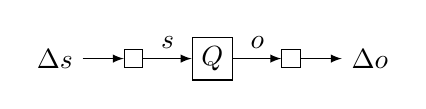
\begin{tikzpicture}[auto,>=latex]
    \node[] (input) {$\Delta s$};
    \node[block, right of=input] (I) {$\I$};
    \node[block, right of=I] (Q) {$Q$};
    \node[block, right of=Q] (D) {$\D$};
    \node[right of=D] (output) {$\Delta o$};
    \draw[->] (input) -- (I);
    \draw[->] (I) -- node (s) {$s$} (Q);
    \draw[->] (Q) -- node (o) {$o$} (D);
    \draw[->] (D) -- (output);
\end{tikzpicture}
\end{center}

If $Q(s) = o$ is a computation, then $\inc{Q}$ performs 
the ``same'' computation as $Q$,
but between streams of changes $\Delta s$ and $\Delta o$.
This is the diagram from the
introduction, substituting $\Delta s$ for the transaction stream $T$, 
and $o$ for the stream of view versions $V$.

Notice that our definition of incremental computation is meaningful only for \emph{streaming}
computations; this is in contrast to classic definitions, e.g.~\cite{gupta-idb95} which
consider only one change.  Generalizing the definition to operate on streams gives us
additional power, especially when operating with recursive queries.

The following proposition is one of our central results.

\begin{proposition}(Properties of the incremental version):\\
\label{prop-inc-properties}
For computations of appropriate types, the following hold:
\begin{description}
\item[inversion:] $Q\mapsto\inc{Q}$ is bijective; its inverse is $Q\mapsto \I\circ Q\circ\D$.
\item[invariance:] $\inc{+} = +, \inc{(\zm)} = \zm, \inc{-} = -, \inc{\I}=\I, \inc{\D}=\D$
\item[push/pull:] 
    $Q \circ \I = \I \circ \inc{Q}$; $\D\circ Q = \inc{Q}\circ\D$
\item[chain:] $\inc{(Q_1\circ Q_2)} = \inc{Q_1}\circ\inc{Q_2}$ (This generalizes to operators with multiple inputs.)
\item[add:] $\inc{(Q_1 + Q_2)} = \inc{Q_1} + \inc{Q_2}$
\item[cycle:] $\inc{(\lambda s. \fix{\alpha}{T(s,\zm(\alpha)}))} = \lambda s. \fix{\alpha}{\inc{T}(s,\zm(\alpha)})$
\end{description}
\end{proposition}
\begin{proof}

The inversion and push-pull properties follow straightforwardly from the fact 
that $\I$ and $\D$ are inverses of each other.

For proving invariance we have $\inc{+}(a, b) \defn \D(\I(a) + \I(b)) = a + b$, due to 
linearity of $\I$.  
$\inc{-}(a) = \D(-\I(a)) = \D(0 - \I(a)) = \D(\I(0) - \I(a)) = \D(\I(0 - a)) = -a$,
also due to linearity of $\I$.

The chain rule follows from push-pull. Indeed, 
$$
\I\circ\inc{Q_1}\circ\inc{Q_2}=Q_1\circ\I\circ\inc{Q_2}=Q_1\circ Q_2\circ\I
$$

I.e., we have the following sequence of equivalent circuits:

\begin{center}
\begin{tabular}{m{7.5cm}m{1cm}}
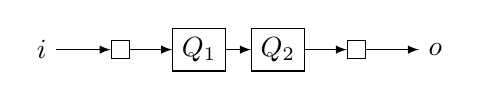
\begin{tikzpicture}[auto,>=latex]
  \node[] (input) {$i$};
  \node[block, right of=input] (I) {$\I$};
  \node[block, right of=I] (Q1) {$Q_1$};
  \node[block, right of=Q1] (Q2) {$Q_2$};
  \node[block, right of=Q2] (D) {$\D$};
  \node[right of=D] (output)  {$o$};
  \draw[->] (input) -- (I);
  \draw[->] (I) -- (Q1);
  \draw[->] (Q1) -- (Q2);
  \draw[->] (Q2) -- (D);
  \draw[->] (D) -- (output);
\end{tikzpicture} 
& $\cong$ \\
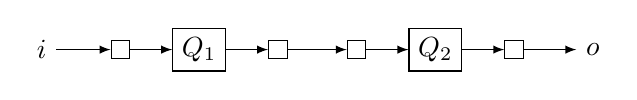
\begin{tikzpicture}[auto,>=latex]
  \node[] (input) {$i$};
  \node[block, right of=input] (I) {$\I$};
  \node[block, right of=I] (Q1) {$Q_1$};
  \node[block, right of=Q1] (D1) {$\D$};
  \node[block, right of=D1] (I1) {$\I$};
  \node[block, right of=I1] (Q2) {$Q_2$};
  \node[block, right of=Q2] (D) {$\D$};
  \node[right of=D] (output)  {$o$};
  \draw[->] (input) -- (I);
  \draw[->] (I) -- (Q1);
  \draw[->] (Q1) -- (D1);
  \draw[->] (D1) -- (I1);
  \draw[->] (I1) -- (Q2);
  \draw[->] (Q2) -- (D);
  \draw[->] (D) -- (output);
\end{tikzpicture} & $\cong$ \\
%\noindent which, due to associativity of function composition, is the same as:
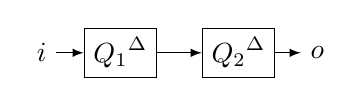
\begin{tikzpicture}[auto,>=latex]
  \node[] (input) {$i$};
  \node[block, right of=input] (Q1) {$\inc{Q_1}$};
  \node[block, right of=Q1, node distance=1.5cm] (Q2) {$\inc{Q_2}$};
  \node[right of=Q2] (output)  {$o$};
  \draw[->] (input) -- (Q1);
  \draw[->] (Q1) -- (Q2);
  \draw[->] (Q2) -- (output);
\end{tikzpicture}
\end{tabular}
\end{center}

Here is a version of the chain rule with a binary operator:

\begin{center}
\begin{tabular}{m{7.5cm}m{1cm}}
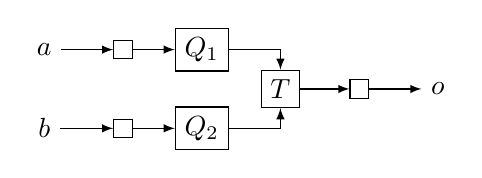
\begin{tikzpicture}[auto,node distance=1cm,>=latex]
    \node[] (a) {$a$};
    \node[block, right of=a] (ai) {$\I$};
    \node[below of=a] (b) {$b$};
    \node[block, right of=b] (bi) {$\I$};
    \node[block, right of=ai] (q1) {$Q_1$};
    \node[below of=q1, node distance=.5cm] (midway) {};
    \node[block, right of=bi] (q2) {$Q_2$};
    \node[block, right of=midway] (q) {$T$};
    \node[block, right of=q] (D) {$\D$};
    \node[right of=D] (output) {$o$};
    \draw[->] (a) -- (ai);
    \draw[->] (b) -- (bi);
    \draw[->] (ai) -- (q1);
    \draw[->] (bi) -- (q2);
    \draw[->] (q1) -| (q);
    \draw[->] (q2) -| (q);
    \draw[->] (q) -- (D);
    \draw[->] (D) -- (output);
\end{tikzpicture}
& $\cong$ \\
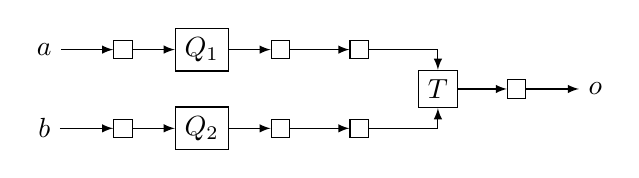
\begin{tikzpicture}[auto,node distance=1cm,>=latex]
    \node[] (a) {$a$};
    \node[block, right of=a] (ai) {$\I$};
    \node[block, right of=ai] (q1) {$Q_1$};
    \node[block, right of=q1] (d1) {$\D$};
    \node[block, right of=d1] (i1) {$\I$};
    
    \node[below of=a] (b) {$b$};
    \node[block, right of=b] (bi) {$\I$};
    \node[block, right of=bi] (q2) {$Q_2$};
    \node[block, right of=q2] (d2) {$\D$};
    \node[block, right of=d2] (i2) {$\I$};
    
    \node[below of=i1, node distance=.5cm] (midway) {};
    \node[block, right of=midway] (q) {$T$};
    \node[block, right of=q] (D) {$\D$};
    \node[right of=D] (output) {$o$};
    \draw[->] (a) -- (ai);
    \draw[->] (ai) -- (q1);
    \draw[->] (q1) -- (d1);
    \draw[->] (d1) -- (i1);
    
    \draw[->] (b) -- (bi);
    \draw[->] (bi) -- (q2);
    \draw[->] (q2) -- (d2);
    \draw[->] (d2) -- (i2);
    
    \draw[->] (i1) -| (q);
    \draw[->] (i2) -| (q);
    \draw[->] (q) -- (D);
    \draw[->] (D) -- (output);
\end{tikzpicture} & $\cong$ \\
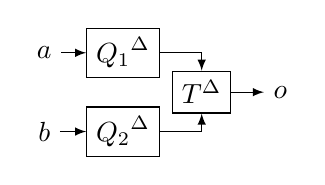
\begin{tikzpicture}[auto,node distance=1cm,>=latex]
    \node[] (a) {$a$};
    \node[below of=a] (b) {$b$};
    \node[block, right of=a] (q1) {$\inc{Q_1}$};
    \node[below of=q1, node distance=.5cm] (midway) {};
    \node[block, right of=b] (q2) {$\inc{Q_2}$};
    \node[block, right of=midway] (q) {$\inc{T}$};
    \node[right of=q] (output) {$o$};
    \draw[->] (a) -- (q1);
    \draw[->] (b) -- (q2);
    \draw[->] (q1) -| (q);
    \draw[->] (q2) -| (q);
    \draw[->] (q) -- (output);
\end{tikzpicture}
\end{tabular}
\end{center}

The add rule follows from push/pull and the linearity of $\I$ (or $\D$). Indeed, 
$$
\I\circ(\inc{Q_1}+\inc{Q_2})=\I\circ\inc{Q_1}+\I\circ\inc{Q_2}=
Q_1\circ\I+ Q_2\circ\I = (Q_1+Q_2)\circ\I
$$

I.e., the following diagrams are equivalent:

\begin{center}
\begin{tabular}{m{6cm}m{1cm}}
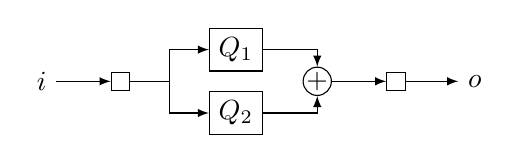
\begin{tikzpicture}[auto,>=latex]
  \node[] (input) {$i$};
  \node[block, right of=input] (I) {$\I$};
  \node[block, above right=0cm and 1cm of I] (Q1) {$Q_1$};
  \node[block, below right=0cm and 1cm of I] (Q2) {$Q_2$};
  \node[block, shape=circle, right of=I, node distance=2.5cm, inner sep=0pt] (plus) {$+$};
  \node[block, right of=plus,node distance=1cm] (D) {$\D$};
  \node[right of=D] (output) {$o$};
  \draw[->] (input) -- (I);
  \draw[<-] (Q1.west) -- ++(-5mm,0) |- (I);
  \draw[<-] (Q2.west) -- ++(-5mm,0) |- (I);
  \draw[->] (Q1) -| (plus);
  \draw[->] (Q2) -| (plus);
  \draw[->] (plus) -- (D);
  \draw[->] (D) -- (output);
\end{tikzpicture} 
& $\cong$ \\ 
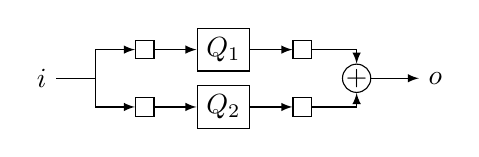
\begin{tikzpicture}[auto,>=latex]
  \node[] (input) {$i$};
  \node[block, above right=0cm and 1cm of input] (I1) {$\I$};
  \node[block, below right=0cm and 1cm of input] (I2) {$\I$};
  \node[block, right of=I1] (Q1) {$Q_1$};
  \node[block, right of=I2] (Q2) {$Q_2$};
  \node[block, right of=Q1] (D1) {$\D$};
  \node[block, right of=Q2] (D2) {$\D$};
  \node[block, shape=circle, right of=input, node distance=4cm, inner sep=0pt] (plus) {$+$};
  \node[right of=plus] (output) {$o$};
  \draw[<-] (I1.west) -- ++(-5mm,0) |- (input);
  \draw[<-] (I2.west) -- ++(-5mm,0) |- (input);
  \draw[->] (I1) -- (Q1);
  \draw[->] (I2) -- (Q2);
  \draw[->] (Q1) -- (D1);
  \draw[->] (Q2) -- (D2);
  \draw[->] (D1) -| (plus);
  \draw[->] (D2) -| (plus);
  \draw[->] (plus) -- (output);
\end{tikzpicture} & $\cong$ \\
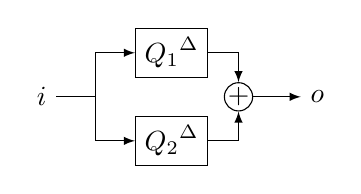
\begin{tikzpicture}[auto,>=latex]
  \node[] (input) {$i$};
  \node[block, above right=0cm and 1cm of input] (Q1) {$\inc{Q_1}$};
  \node[block, below right=0cm and 1cm of input] (Q2) {$\inc{Q_2}$};
  \node[block, shape=circle, right of=input, node distance=2.5cm, inner sep=0pt] (plus) {$+$};
  \node[right of=plus] (output) {$o$};
  \draw[<-] (Q1.west) -- ++(-5mm,0) |- (input);
  \draw[<-] (Q2.west) -- ++(-5mm,0) |- (input);
  \draw[->] (Q1) -| (plus);
  \draw[->] (Q2) -| (plus);
  \draw[->] (plus) -- (output);
\end{tikzpicture} 
\end{tabular}
\end{center}

The cycle rule is most interesting. First, observe that if $T$ is causal then so is 
$\inc{T}$ thus both sides of the
equality are well-defined. Next, we can use again push/pull to show the equality 
if we can check that
$$
\I\circ(\lambda s. \fix{\alpha}{\inc{T}(s,\zm(\alpha)}) =
(\lambda s. \fix{\alpha}{T(s,\zm(\alpha)})\circ\I
$$
that is, for any $s$,
$$
\I(\fix{\alpha}{\inc{T}(s,\zm(\alpha)}) =
\fix{\alpha}{T(\I(s),\zm(\alpha)})
$$
This follows from the following lemma.
\end{proof}

\begin{lemma}
\label{lemma-delta-fix}
If the parameters $a$ and $b$ are related by $b=\D(a)$ (equivalently $a=\I(b)$)
then the unique solutions of the fixed point equations
$$
\alpha~=~ T(a,\zm(\alpha))~~~~\mbox{and}~~~~
\beta~=~\inc{T}(b,\zm(\beta))
$$
are related by $\alpha=\I(\beta)$ (equivalently $\beta=\D(\alpha)$). 
\end{lemma}
\begin{proof} (Of Lemma~\ref{lemma-delta-fix})
Let $\beta$ be the unique solution of $\beta~=~\inc{T}(\D(a),\zm(\beta))$. We verify that
$\alpha=\I(\beta)$ satisfies the equation $\alpha~=~ T(a,\zm(\alpha))$. Indeed, using the fact that $\I$ and $\D$ are inverses as well as the time-invariance of $\I$ we have
\begin{eqnarray*}
\I(\beta) & = & \I(\inc{T}(\D(a),\zm(\beta)))\\
          & = & \I(\D(T(\I(\D(a)),\I(\zm(\beta))))\\
          & = & T(a,\I(\zm(\beta))\\
          & = & T(a,\zm(\I(\beta))
\end{eqnarray*}

I.e., starting from this diagram we apply a sequence of term-rewriting se\-man\-tics-preserving 
transformations:

\begin{center}
\begin{tabular}{m{5.5cm}m{1cm}}
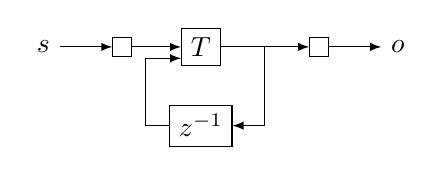
\begin{tikzpicture}[>=latex]
    \node[] (input) {$s$};
    \node[block, right of=input] (I) {$\I$};
    \node[block, right of=I] (f) {$T$};
    \node[block, right of=f, node distance=1.5cm] (D) {$\D$};
    \node[right of=D] (output) {$o$};
    \node[block, below of=f] (z) {$\zm$};
    \draw[->] (input) -- (I);
    \draw[->] (I) -- (f);
    \draw[->] (f) -- node (mid) {} (D);
    \draw[->] (mid.center) |-  (z);
    \draw[->] (z.west) -- ++(-.3,0) |- ([yshift=1mm]f.south west);
    \draw[->] (D) -- (output);
\end{tikzpicture} & $\cong$ \\
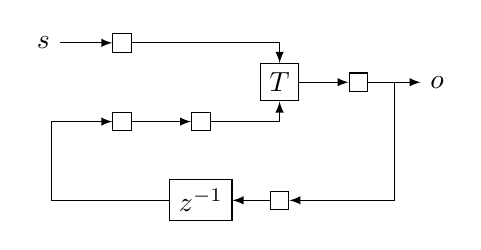
\begin{tikzpicture}[>=latex]
    \node[] (input) {$s$};
    \node[block, right of=input] (I) {$\I$};
    \node[block, below of=I] (D0) {$\D$};
    \node[block, right of=D0] (I0) {$\I$};
    \node[above of=I0, node distance=.5cm] (midway) {};
    
    \node[block, right of=midway] (f) {$T$};
    \node[block, right of=f] (D) {$\D$};
    \node[right of=D] (output) {$o$};
    \node[block, below of=f, node distance=1.5cm] (I1) {$\I$};
    \node[block, left of=I1] (z) {$\zm$};
    \draw[->] (input) -- (I);
    \draw[->] (I) -| (f);
    \draw[->] (D0) -- (I0);
    \draw[->] (I0) -| (f);
    \draw[->] (f) -- (D);
    \draw[->] (D) -- node (mid) {} (output);
    \draw[->] (mid.center) |-  (I1);
    \draw[->] (I1) -- (z);
    \draw[->] (z.west) -- ++(-1.5,0) |- (D0);
\end{tikzpicture} & $\cong$ \\
\begin{tikzpicture}[>=latex]
    \node[] (input) {$s$};
    \node[block, right of=input] (f) {$\inc{T}$};
    \node[right of=f, node distance=1.5cm] (output) {$o$};
    \node[block, below of=f] (z) {$\zm$};
    \draw[->] (input) -- (f);
    \draw[->] (f) -- node (mid) {} (output);
    \draw[->] (mid.center) |-  (z);
    \draw[->] (z.west) -- ++(-.3,0) |- ([yshift=1mm]f.south west);
\end{tikzpicture}
\end{tabular}
\end{center}

\end{proof}

If we specialize the above formula for the case $T(a,b) = Q(a+b)$ 
(for some time-invariant operator $Q$), by us the linearity of $\I$
we get that:

\noindent
\begin{tabular}{m{6cm}m{0.5cm}m{4cm}}
\begin{tikzpicture}[auto,>=latex]
  \node[] (input) {$i$};
  \node[block, right of=input] (I0) {$\I$};
  \node[block, shape=circle, right of=I0, inner sep=0in] (plus) {$+$};
  \node[block, right of=plus] (q) {$Q$};
  \node[block, right of=q, node distance=1.5cm] (D) {$\D$};
  \node[right of=D] (output)  {$o$};
  \draw[->] (input) -- (I0);
  \draw[->] (I0) -- (plus);
  \draw[->] (plus) -- (q);
  \draw[->] (q) -- node (o) {} (D);
  \draw[->] (D) -- (output);
  \node[block, below of=q] (z) {$\zm$};
  \draw[->] (o) |- (z);
  \draw[->] (z) -| (plus);
\end{tikzpicture} & $\cong$ &
\begin{tikzpicture}[auto,>=latex]
  \node[] (input) {$i$};
  \node[block, shape=circle, right of=input, inner sep=0in] (plus) {$+$};
  \node[block, right of=plus] (q) {$\inc{Q}$};
  \node[right of=q, node distance=1.5cm] (output)  {$o$};
  \draw[->] (input) -- (plus);
  \draw[->] (plus) -- (q);
  \draw[->] (q) -- node (o) {} (output);
  \node[block, below of=q] (z) {$\zm$};
  \draw[->] (o) |- (z);
  \draw[->] (z) -| (plus);
\end{tikzpicture} 
\end{tabular}

\begin{comment}
& \mbox{Initial form} \\
\begin{tikzpicture}[auto,>=latex]
  \node[] (input) {$i$};
  \node[block, right of=input] (D0) {$\D$};
  \node[block, right of=D0] (I0) {$\I$};
  \node[block, shape=circle, right of=I0, inner sep=0in] (plus) {$+$};
  \node[block, right of=plus] (q) {$Q$};
  \node[right of=q, node distance=4cm] (output)  {$o$};
  \draw[->] (input) -- (D0);
  \draw[->] (D0) -- (I0);
  \draw[->] (I0) -- (plus);
  \draw[->] (plus) -- (q);
  \draw[->] (q) -- node [pos=0.8] (o) {} (output);
  \node[block, below of=q] (I1) {$\I$};
  \node[block, right of=I1] (D1) {$\D$};
  \node[block, right of=D1] (z) {$\zm$};
  \draw[->] (o) |- (z);
  \draw[->] (z) -- (D1);
  \draw[->] (D1) -- (I1);
  \draw[->] (I1) -| (plus);
\end{tikzpicture} & \I \circ \D = \id \\
\begin{tikzpicture}[auto,>=latex]
  \node[] (input) {$i$};
  \node[block, right of=input] (D0) {$\D$};
  \node[block, shape=circle, right of=D0, inner sep=0in] (plus) {$+$};
  \node[block, right of=plus] (I) {$\I$};
  \node[block, right of=I] (q) {$Q$};
  \node[right of=q, node distance=2cm] (output)  {$o$};
  \draw[->] (input) -- (D0);
  \draw[->] (D0) -- (plus);
  \draw[->] (plus) -- (I);
  \draw[->] (I) -- (q);
  \draw[->] (q) -- node (o) {} (output);
  \node[block, below of=I] (z) {$\zm$};
  \node[block, right of=z] (D1) {$\D$};
  \draw[->] (o) |- (D1);
  \draw[->] (D1) -- (z);
  \draw[->] (z) -| (plus);but not
\end{tikzpicture} & \mbox{Linearity of }\I  \\
\begin{tikzpicture}[auto,>=latex]
  \node[] (input) {$i$};
  \node[block, right of=input] (D0) {$\D$};
  \node[block, shape=circle, right of=D0, inner sep=0in] (plus) {$+$};
  \node[block, right of=plus] (I) {$\I$};
  \node[block, right of=I] (q) {$Q$};
  \node[block, right of=q] (D1) {$\D$};
  \node[block, right of=D1] (I2) {$\I$};
  \node[right of=I2, node distance=2cm] (output)  {$o$};
  \draw[->] (input) -- (D0);
  \draw[->] (D0) -- (plus);
  \draw[->] (plus) -- (I);
  \draw[->] (I) -- (q);
  \draw[->] (q) -- (D1);
  \draw[->] (D1) -- (I2);
  \draw[->] (I2) -- node (o) {} (output);
  \node[block, below of=I] (z) {$\zm$};
  \node[block, right of=z] (D1) {$\D$};
  \draw[->] (o) |- (D1);
  \draw[->] (D1) -- (z);
  \draw[->] (z) -| (plus);
\end{tikzpicture} & \D \circ \I = \id \\
\end{comment}


%\subsection{Linear operators}

\begin{theorem}[Linear]\label{linear}
For any LTI operator $Q$ we have $\inc{Q}=Q$.
\end{theorem}

\begin{proof}
By the push/pull rule from Proposition~\ref{prop-inc-properties} 
it suffices to show that $Q$ commutes with differentiation:
$$
\begin{aligned}
  \D(Q(s)) &= Q(s)-\zm(Q(s)) & \mbox{by definition of }\D \\
  &= Q(s)-Q(\zm(s)) & \mbox{by time-invariance of }Q \\
  &= Q(s-\zm(s)) & \mbox{by linearity of }Q \\
  &= Q(\D(s)) & \mbox{by definition of }\D.
\end{aligned}
$$
\end{proof}


As we have shown, the incremental version of a linear unary operator equals the operator itself.
However, this is not true, in general, for multilinear operators. Nonetheless, there is a useful relationship
between the incremental version of a multilinear operator and the operator itself. We illustrate with bilinear
operators. 
\begin{comment}
\val{Such as join. from incremental maintenance literature recall the definition of "delta" for join:
$\Delta(R\bowtie S) = R\bowtie(\Delta S) \cup (\Delta R)\bowtie S \cup (\Delta R)\bowtie(\Delta S)$.}
\mihai{Indeed, the join is the main application.  Should we hint at this?  It's the first
time the relational algebra will appear in this text.}
\end{comment}

\begin{theorem}[Bilinear]\label{bilinear}
For any bilinear time-invariant operator $\times$ we have
$\inc{(a \times b)} ~=~ a \times b ~+~ \I(\zm(a)) \times b ~+~ a \times \I(\zm(b))$.
\end{theorem}

By rewriting this statement using $\Delta a$ for the stream of changes to $a$ we
get the familiar formula for incremental joins:
$\Delta(a\times b) =\Delta a \times \Delta b + a\times(\Delta b) + (\Delta a)\times b$.

In other words, the following two diagrams are equivalent:

\begin{tabular}{m{4.5cm}m{1cm}m{4.5cm}}
\begin{tikzpicture}[auto,node distance=1cm,>=latex]
    \node[] (a) {$a$};
    \node[block, right of=a] (ai) {$\I$};
    \node[below of=a, node distance=.8cm] (midway) {};
    \node[below of=midway, node distance=.8cm] (b) {$b$};
    \node[block, right of=b] (bi) {$\I$};
    \node[block, right of=midway, node distance=2cm] (q) {$\times$};
    \node[block, right of=q] (D) {$\D$};
    \node[right of=D] (output) {$o$};
    \draw[->] (a) -- (ai);
    \draw[->] (b) -- (bi);
    \draw[->] (ai) -| (q);
    \draw[->] (bi) -| (q);
    \draw[->] (q) -- (D);
    \draw[->] (D) -- (output);
\end{tikzpicture} &
$\cong$ &
\begin{tikzpicture}[auto,>=latex]
  \node[] (input1) {$a$};
  \node[below of=input1, node distance=2cm] (input2) {$b$};
  \node[block, right of=input1] (I1) {$\I$};
  \node[block, below of=I1] (ab) {$\times$};
  \node[block, right of=input2] (I2) {$\I$};
  \draw[->] (input1) -- node[name=i1tap] {} (I1);
  \draw[->] (input2) -- node[name=i2tap,below] {} (I2);
  \draw[->] (i1tap) |- ([yshift=-1mm]ab.north west);
  \draw[->] (i2tap) |- ([yshift=1mm]ab.south west);
  \node[block, right of=I1] (ZI1) {$\zm$};
  \node[block, right of=I2] (ZI2) {$\zm$};
  \draw[->] (I1) -- (ZI1);
  \draw[->] (I2) -- (ZI2);
  \node[block, right of=ZI1] (DI1) {$\times$};
  \node[block, right of=ZI2] (DI2) {$\times$};
  \draw[->] (ZI1) -- (DI1);
  \draw[->] (ZI2) -- (DI2);
  \node[block, circle, right of=ab, inner sep=0cm, node distance=2cm] (sum) {$+$};
  \draw[->] (ab) -- (sum);
  \draw[->] (DI1) -- (sum);
  \draw[->] (DI2) -- (sum);
  \node[right of=sum] (output) {$o$};
  \draw[->] (sum) -- (output);
  \draw[->] (i1tap.south) -- (DI2);
  \draw[->] (i2tap.north) -- (DI1);
\end{tikzpicture}
\end{tabular}
\begin{proof}
$$
\begin{aligned}
\inc{(a \times b)} &= \D(\I(a) \times \I(b)) & \mbox{def of } \inc{\cdot} \\
             &= (\I(a) \times \I(b)) ~-~  \zm(\I(a) \times \I(b)) & \mbox{def of } \D \\
             &= \I(a) \times \I(b) ~-~  \zm(\I(a)) \times \zm(\I(b)) & \times \mbox{ time inv.}\\
             &= \I(a) \times \I(b) ~-~  \zm(\I(a)) \times \I(b) & \mbox{ add and sub a term} \\
             & ~~~~~~~~~~~~+~ \zm(\I(a)) \times \I(b) ~-~ \zm(\I(a)) \times \zm(\I(b))) & \\
             &= \D(\I(a)) \times \I(b) ~+~ \zm(\I(a)) \times \D(\I(b))) & \mbox{bilinearity, def of }\D \\ 
             &= a \times \I(b) ~+~ \zm(\I(a)) \times b & \D \circ \I = \id \\ 
             &= a \times \I(b) ~-~ a \times \zm(\I(b)) & \mbox{ add and sub a term} \\
             &     ~~~~~~~~~~~~~~+~ a \times \zm(\I(b)) ~+~ \zm(\I(a)) \times b & \\        
             &= a \times \D(\I(b)) ~+~ a \times \zm(\I(b)) ~+~ \zm(\I(a)) \times b & \mbox{bilinearity, def of }\D  \\     
             &= a \times b  ~+~ \zm(\I(a)) \times b ~+~ a \times \zm(\I(b)) 
\end{aligned}
$$
\end{proof}

\subsection{Vector representations}\label{sec:vector-picture}

Some formulas are easier to read as mathematical expressions over ``vectors''.
We will use the following representation to depict a fragment of a stream $s$:

$\strm{0}{0}$

This ``vector'' representation fixes a time $t$ and shows the integral of the stream prefix
up to $\I(s)[t-1]$ as a rectangle, and $s[t]$ as a square.  We will use a grey rectangle to 
show which part of a stream participates in a computation.  For example, we have the following
notations:

$$
\begin{aligned}
\strm{0 0} &= 0 \\
\strm{0 1} &= s[t] \\
\strm{1 0} &= \I(s)[t-1] = \zm(\I(s))[t] \\
\strm{1 1} &= \I(s)[t-1] + s[t] = \I(s)[t] 
\end{aligned}
$$

Using this notation, the incremental version of a function $f$ is defined
as $\inc{f}(\strm{0}{1}) = f(\strm{1}{1}) - f(\strm{1}{0})$.

Theorem~\ref{linear} states that for a linear function $f$ we have: \\
$f(\strm{1 1}) - f(\strm{1 0}) = f(\strm{0 1}).$

The statement of Theorem~\ref{bilinear}, for a bilinear stream operation 
$\times$ can be written as:
$$
\begin{aligned}
\strm{1 1} \times \strm{1 1} = & 
\matmult{\strm{1 0}}{\strm{1 0}} \\ + & 
\matmult{\strm{1 0}}{\strm{0 1}} \\ + & 
\matmult{\strm{0 1}}{\strm{1 0}} \\ + & 
\matmult{\strm{0 1}}{\strm{0 1}}.
\end{aligned}
$$

By definition $\inc{\times}$ is: 
$$
\begin{aligned}
\matmult{\strm{1 1}}{\strm{1 1}} - \\
\matmult{\strm{1 0}}{\strm{1 0}} = &
\matmult{\strm{1 0}}{\strm{0 1}} \\ + & 
\matmult{\strm{0 1}}{\strm{1 0}} \\ + & 
\matmult{\strm{0 1}}{\strm{0 1}}.
\end{aligned}
$$

\section{Nested streams}

\subsection{Creating and destroying streams}\label{sec:stream-intro-elim}

We introduce two new stream operators that are instrumental in
expressing recursive query evaluation.  These operators allow us
to build circuits implementing looping constructs, which 
are used to iterate computations until a fixed-point is reached.

\subsubsection{Generalizing box-and-arrow diagrams}

From now on our circuits will mix computations on scalars and streams.
We will use the same graphical representation for functions that compute
on scalars: boxes with input and output arrows.  The values on the
the connecting arrows will be scalars instead of streams; otherwise
the interpretation of boxes as function application is unchanged.

When connecting boxes the types of the arrows must match.  E.g.,
the output of a box producing a stream cannot be connected to the
input of a box consuming a scalar.

\subsubsection{Stream introduction}\label{sec:stream-introduction}

\begin{definition}[Dirac delta]
The delta function (named from the Dirac delta function) $\delta_0 : A \rightarrow \stream{A}$
produces a stream from a scalar value.  
The output stream is produced as follows from the input scalar:

$$\delta_0(v)[t] \defn \left\{
\begin{array}{ll}
  v & \mbox{if } t = 0 \\
  0_A & \mbox{ otherwise}
\end{array}
\right.
$$
\end{definition}

Here is a diagram showing a $\delta_0$ operator; note that the input is a scalar value,
while the output is a stream:  

\begin{center}
\begin{tikzpicture}[auto,node distance=1cm,>=latex]
    \node[] (input) {$i$};
    \node[block, right of=input] (delta) {$\delta_0$};
    \node[right of=delta] (output) {$o$};
    \draw[->] (input) -- (delta);
    \draw[->] (delta) -- (output);
\end{tikzpicture}
\end{center}

For example, $\delta_0(5)$ is the stream $\sv{5 0 0 0 0}$.

\subsubsection{Stream elimination}\label{sec:stream-elimination}

Recall that $\streamf{A}$ was defined in Definition~\ref{def:zae} to be the set of 
$A$-streams over a group $A$ that are zero almost everywhere. 

\begin{definition}[indefinite integral]
We define a function $\int : \streamf{A} \rightarrow
A$ as $\int(s) \defn \sum_{t \geq 0} s[t]$.
\end{definition}

$\int$ is closely related to $\I$; if $\I$ is the
indefinite integral, $\int$ is the definite integral on the
interval $0 - \infty$.   Unlike $\I$
$\int$ produces a scalar value, the ``last'' distinct value that would
appear in the stream produced by $\I$.
For example $\int(\cut{\id}{4}) = 0 + 1 + 2 + 3 = 6$, because
$\I(\cut{\id}{4}) = \sv{0 1 3 6 6}$.

An alternative definition for $\int$ for all streams $\stream{A}$
would extend the set $A$ with an ``infinite'':
$\overline{A} \defn A \cup \{ \top \}$, and define $\int{s} \defn
\top$ for streams that are not zero a.e., $s \in \stream{A} \setminus \streamf{A}$.

Here is a diagrams showing the $\int$ operator; note that  the result it 
produces is a scalar, and not a stream:

\begin{center}
\begin{tikzpicture}[auto,node distance=1cm,>=latex]
    \node[] (input) {$i$};
    \node[block, right of=input] (S) {$\int$};
    \node[right of=S] (output) {$o$};
    \draw[->] (input) -- (S);
    \draw[->] (S) -- (output);
\end{tikzpicture}
\end{center}

$\delta_0$ is the left inverse of $\int$, i.e., the
following equation holds: $\int \circ \;\delta_0 = \id_A$.  

\subsubsection{The $E$ and $X$ operators}

The composition $\I \circ \delta_0$ is frequently used, so we 
will give it a name, denoting it by $E: A \to \stream{A}$, $E \defn \I \circ \delta_0$.

\begin{center}
\begin{tabular}{m{2cm}m{.5cm}m{4cm}}
\begin{tikzpicture}[auto,>=latex]
  \node[] (input) {};
  \node[block, right of=input] (E) {$E$};
  \node[right of=E] (output) {};
  \draw[->] (input) -- (E);
  \draw[->] (E) -- (output);
\end{tikzpicture} &
$\defn$ &
\begin{tikzpicture}[auto,>=latex]
  \node[] (input) {};
  \node[block, right of=input] (delta) {$\delta_0$};
  \node[block, right of=delta] (i) {$\I$};
  \node[right of=i] (output) {};
  \draw[->] (input) -- (delta);
  \draw[->] (delta) -- (i);
  \draw[->] (i) -- (output);
\end{tikzpicture}
\end{tabular}
\end{center}

Notice that the output of the $E$ operator is a constant infinite stream, consisting the scalar
value at the input.  $E(5) = \sv{5 5 5 5 5}$.

Similarly, we denote by $X: \stream{A} \to A$ the combination $X \defn \int \circ \D$. 

\begin{center}
\begin{tabular}{m{2cm}m{.5cm}m{4cm}}
\begin{tikzpicture}[auto,>=latex]
  \node[] (input) {};
  \node[block, right of=input] (X) {$X$};
  \node[right of=X] (output) {};
  \draw[->] (input) -- (X);
  \draw[->] (E) -- (output);
\end{tikzpicture} &
$\defn$ &
\begin{tikzpicture}[auto,>=latex]
  \node[] (input) {};
  \node[block, right of=input] (D) {$\D$};
  \node[block, right of=D] (i) {$\int$};
  \node[right of=i] (output) {};
  \draw[->] (input) -- (D);
  \draw[->] (D) -- (i);
  \draw[->] (i) -- (output);
\end{tikzpicture}
\end{tabular}
\end{center}

\begin{proposition}
For a monotone stream $o \in \stream{A}$ we have 
$X(o) = \lim_{n \to \infty} o[n]$, if the limit exists.
\end{proposition}
\begin{proof}
$X(\cut{o}{n}) = (\int \circ \D)(\cut{o}{n}) = o[0] + (o[1] - o[0]) + \ldots + (o[n] - o[n-1]) = o(n)$.
The result follows by taking limits on both sides.
\end{proof}
\mihai{This looks almost right, but it is not.}

Clearly, $E$ is the left-inverse of $X$.

\begin{proposition}
$\delta_0$, $\int$, $E$, and $X$ are LTI.
\end{proposition}
\begin{proof}
The proof is easy using simple algebraic manipulation of the definitions of these operators.
\end{proof}

\subsubsection{Time domains}\label{sec:time-domains}

So far we had the tacit assumption that ``time'' is common for all
streams in a program.  For example, when we add two streams, 
we assume that they use the same ``clock'' for the time dimension.
However, the $\delta_0$ operator creates a streams with a ``new'', independent time
dimension.  In Section~\ref{sec:wfc} we will define some well-formed circuit
construction rules that will ensure that such time domains are always ``insulated'', 
by requiring each diagram that starts with a $\delta_0$ operator
to end with a corresponding $\int$ operator:

\begin{center}
\begin{tikzpicture}[auto,node distance=1cm,>=latex]
    \node[] (input) {$i$};
    \node[block, right of=input] (delta) {$\delta_0$};
    \node[block, right of=delta] (f) {$Q$};
    \draw[->] (input) -- (delta);
    \draw[->] (delta) -- (f);

    \node[block, right of=f] (S) {$\int$};
    \node[right of=S] (output) {$o$};
    \draw[->] (f) -- (S);
    \draw[->] (S) -- (output);
\end{tikzpicture}
\end{center}


\begin{proposition}
If $Q$ is time-invariant, the circuit above has the zero-preservation
property: $\zpp{\int \circ\; Q \circ \delta_o}$.
\end{proposition}
\begin{proof}
  This follows from the fact that all three operators preserve zeros, and thus so 
  does their composition.
\end{proof}

\subsection{Streams of streams}\label{sec:nested}

\subsubsection{Defining nested streams}

Since all streams we work with are defined over abelian groups
and streams themselves form an abelian group, as pointed in Section~\ref{sec:abelianstreams},
it follows that we can naturally define streams of streams.
$\stream{\stream{A}} = \N \rightarrow (\N \rightarrow A)$.  This construction
can be iterated, but our applications do not require more than 
two-level nesting.  Box-and-arrow diagrams can be used equally to
depict functions computing on nested streams; in this case an
arrow represent a stream where each value is another stream.

\newcommand{\ssa}[1]{
\setsepchar{ }
\readlist\arg{#1}
\begin{bmatrix}
   \begin{array}{ccccccc}
        {[} & \arg[1] & \arg[2] & \arg[3] & \arg[4] & \cdots & {]} \\
        {[} & \arg[5] & \arg[6] & \arg[7] & \arg[8] & \cdots & {]} \\
        {[} & \arg[9] & \arg[10] & \arg[11] & \arg[12] & \cdots & {]} \\
        {[} & \arg[13] & \arg[14] & \arg[15] & \arg[16] & \cdots & {]} \\
        \multicolumn{7}{c}{\vdots}
   \end{array}
\end{bmatrix}
}

Equivalently, a nested stream in $\stream{\stream{A}}$ is a value in
$\N \times \N \to A$, i.e., a ``matrix''
with an infinite number of rows, where each row is a stream.  
For example, we can depict the nested stream 
$i \in \stream{\stream{\N}}$ defined by $i[t_0][t_1] = t_0 + 2 t_1$ as:
$$ i = \ssa{0 1 2 3 2 3 4 5 4 5 6 7 6 7 8 9} $$

\noindent ($t_0$ is the column index, and $t_1$ is the row index).

\subsubsection{Lifting stream operators}

We have originally defined lifting (Section~\ref{sec:lifting}) for scalar functions.
We can generalize lifting to apply to stream operators as well.  Consider a 
stream operator $S: \stream{A} \to \stream{B}$.  We define $\lift{S}: \stream{\stream{A}} 
\to \stream{\stream{B}}$ as: $(\lift{S}(s))[t_0][t_1] \defn S(s[t_0])[t_1], \forall t_0, t_1 \in
\N$.  Alternatively, we can write $(\lift{S})(s) = S \circ s$.

In particular, a scalar function $f: A \rightarrow B$ can be can lifted twice to 
produce an operator between streams of streams: $\lift{\lift{f}}: \stream{\stream{A}} 
\rightarrow \stream{\stream{B}}$.

Lifting twice a scalar function computes on elements of the matrix pointwise:

$$(\lift{\lift{(x \mapsto x \bmod 2)}})(i) = 
  \ssa{0 1 0 1 0 1 0 1 0 1 0 1 0 1 0 1}
$$

$\zm$ delays the rows of the matrix:

$$\zm(i) = \ssa{0 0 0 0 0 1 2 3 2 3 4 5 4 5 6 7}$$

\noindent while its lifted counterpart delays each column of the matrix:

$$(\lift{\zm})(i) = \ssa{0 0 1 2 0 2 3 4 0 4 5 6 0 6 7 8}$$

We can also apply both operators, and they commute:

$$(\lift{\zm})(\zm(i)) = \zm((\lift{\zm})(i)) = \ssa{0 0 0 0 0 0 1 2 0 2 3 4 0 4 5 6}$$

Similarly, we can apply $\D$ to nested streams $\D : \stream{\stream{A}} \to
\stream{\stream{A}}$, computing on rows of the matrix:

$$\D(i) = \ssa{0 1 2 3 2 2 2 2 2 2 2 2 2 2 2 2}$$

\noindent while $\lift{\D} : \stream{\stream{A}} \to \stream{\stream{A}}$
computes on the columns:

$$(\lift{\D})(i) = \ssa{0 1 1 1 2 1 1 1 4 1 1 1 6 1 1 1}$$

Similarly, we can apply both differentiation operators in sequence:

$$(\D(\lift{\D}))(i) = \ssa{0 1 1 1 2 0 0 0 2 0 0 0 2 0 0 0}$$

\subsubsection{Matrix representations of nested streams}\label{sec:matrix-picture}

Similar to the vector graphical representations from \refsec{sec:vector-picture},
we can use a graphical representation of a nested stream $s$:

$\mtrx{0 0 0 0}$

The four rectangles correspond to the following expressions: 
$$
\begin{aligned}
\I(\lift{\I}(s))[t_0-1][t_1-1] = \I(\zm(\lift{\I}(\lift{\zm})))[t_0][t_1] =& \mtrx{1 0 0 0} \\
\I(s)[t_0][t_1-1] = \I(\zm(s))[t_0][t_1] =& \mtrx{0 1 0 0} \\
\lift{\I(s)}[t_0-1][t_1] = \lift{\I(\lift{\zm})}(s)[t_0][t_1] =& \mtrx{0 0 1 0} \\
s[t_0][t_1] =& \mtrx{0 0 0 1}.
\end{aligned}
$$

Lifting a vector we obtain a matrix, e.g.:
$\lift{\strm{1 0}} = \mtrx{1 0 1 0}$. 

Consider a bilinear scalar operator $\times$.  Let us expand the following expression:
$\inc{(\lift{(\inc{(\lift{(a \times b)})})})}$.

In Section~\ref{sec:vector-picture} we expanded the inner term
$$
\begin{aligned}
\inc{(\lift{a \times b})} = &\matmult{\strm{1 0}}{\strm{0 1}} \\ 
&\matmult{\strm{0 1}}{\strm{1 0}} \\
&\matmult{\strm{0 1}}{\strm{0 1}}
\end{aligned}
$$

Lifting this term again we get:

$$
\begin{aligned}
\lift{(\inc{(\lift{(a \times b)})})} =& 
\matmult{\mtrx{1 0 1 0}}{\mtrx{0 1 0 1}} +\\ 
&\matmult{\mtrx{0 1 0 1}}{\mtrx{1 0 1 0}} +\\
&\matmult{\mtrx{0 1 0 1}}{\mtrx{0 1 0 1}}
\end{aligned}
$$

And now we apply incrementalize this again, by expanding each
term into 3 other terms and regrouping due to distributivity of $\times$ over addition (bilinearity):

$$
\begin{aligned}
\inc{(\lift{(\inc{(\lift{(a \times b)})})})} = \\ 
%
\matmult{\mtrx{1 0 0 0}}{\mtrx{0 0 0 1}} + 
\matmult{\mtrx{0 0 1 0}}{\mtrx{0 1 0 0}} + \\
\matmult{\mtrx{0 0 1 0}}{\mtrx{0 0 0 1}} + \\ 
%
\matmult{\mtrx{0 1 0 0}}{\mtrx{0 0 1 0}} +
\matmult{\mtrx{0 0 0 1}}{\mtrx{1 0 0 0}} +\\
\matmult{\mtrx{0 0 0 1}}{\mtrx{0 0 1 0}} +\\
%
\matmult{\mtrx{0 1 0 0}}{\mtrx{0 0 0 1}} +
\matmult{\mtrx{0 0 0 1}}{\mtrx{0 1 0 0}} + \\
\matmult{\mtrx{0 0 0 1}}{\mtrx{0 0 0 1}} = \\
%
\matmult{\mtrx{1 1 1 1}}{\mtrx{0 0 0 1}} + 
\matmult{\mtrx{0 0 1 1}}{\mtrx{0 1 0 0}} + \\
\matmult{\mtrx{0 0 0 1}}{\mtrx{1 0 0 0}} + 
\matmult{\mtrx{0 1 0 1}}{\mtrx{0 0 1 9}}.
\end{aligned}
$$

\subsubsection{Strict operators on nested streams}

In order to show that operators defined using feedback are well-defined on
nested streams we need to extend the notion of strict operators from Section~\ref{sec:causal}.

We define a partial order over timestamps: $(i_0, i_1)
\leq (t_0, t_1)$ iff $i_0 \leq t_0$ and $i_1 \leq t_1$.  We extend the
definition of strictness for operators over nested streams: a stream operator
$F: \stream{\stream{A}} \to \stream{\stream{B}}$ is strict if for any $s, s' \in
\stream{\stream{A}}$ and all times $t, i \in \N \times \N$ we have $\forall i <
t, s[i] = s'[i]$ implies $F(s)[t] = F(s')[t]$.
Proposition~\ref{prop-unique-fix} holds for this notion of strictness, i.e., the fixed point operator $\fix{\alpha}{F(\alpha)}$ is well defined for a strict operator $F$.
\mihai{Should write down this proof.}

\begin{proposition}\label{prop-liftz}
The operator $\lift{\zm}: \stream{\stream{A}} \to \stream{\stream{A}}$ is strict.
\end{proposition}

The $\I$ operator on $\stream{\stream{A}}$ is well-defined: it operates on rows
of the matrix, treating each row as a single value:

$$\I(i) = \ssa{0 1 2 3 2 4 6 8 6 9 12 15 12 16 20 24}$$

With this extended notion of strictness we have that the lifted integration operator
is also well-defined: $\lift{\I}: \stream{\stream{A}} \to \stream{\stream{A}}.$
This operator integrates each column of the stream matrix:

$$(\lift{\I})(i) = \ssa{0 1 3 6 2 5 9 14 4 9 15 22 6 13 21 30}$$

Notice the following commutativity properties for integration and differentiation 
on nested streams: $\I \circ (\lift{\I}) = (\lift{\I}) \circ \I$ and 
$\D \circ (\lift{\D}) = (\lift{\D}) \circ \D$.

\begin{comment}
\subsection{Multidimensional integrals and derivatives}

We now define a generalized form of the $\I$ and $\D$ operators to compute on 
streams nested arbitrarily deep.  
We define these operators inductively on the structure of the type $A$ of elements that
they compute on, as follows:

\begin{definition}[Generalized integration] The generalized integration operator
for values of type $A$ is denoted by $\I_A: A \to A$ and is defined as follows: 
$$
\begin{aligned}
\I_A &\defn \id & \mbox{ when $A$ is a scalar type}, \\
\I_{\stream{A}} &\defn \I \circ \lift{\I_A} & \mbox{otherwise.} 
\end{aligned}
$$
\end{definition}


\begin{definition}[Generalized differentiation] The generalized differentiation operator
for values of type $A$ is denoted by $\D_A: A \to A$ and is defined as follows:
$$
\begin{aligned}
\D_A &\defn \id & \mbox{when $A$ is a scalar type,} \\
\D_{\stream{A}} &\defn \lift{\D_A} \circ \D &\mbox{otherwise}
\end{aligned}
$$
\end{definition}


$$\I_{\stream{\stream{\N}}}(i) = ((\lift{\I})(\I))(i)= \ssa{0 1 3 6 2 6 12 20 6 15 27 42 12 28 48 72}$$


Recall the definition we gave for the incremental version of an operator $Q: \stream{A} \to \stream{B}$
in Section~\ref{sec:incremental}: $\inc{Q} = \D \circ Q \circ \I$.  We want to generalize this
definition so that it applies to arbitrary functions on streams of various nesting depths.

\begin{definition}
The incremental version of a function $f: A \to B$ is a function $\inc{f}: A \to B$ defined as 
$\inc{f} \defn \D_B \circ f \circ \I_A$.
\end{definition}

Clearly, this definition generalizes the one we gave before.

Let us compute the incremental version of a twice-lifted scalar operator:
$\inc{(\lift{\lift{f}})} = \D \circ (\lift{\D}) \circ
(\lift{\lift{f}}) \circ (\lift{\I}) \circ \I$.

This definition allows us to talk about the incremental forms of
the two special stream creation and destruction operators from Section~\ref{sec:stream-intro-elim}:

$\inc{\delta_0} = \D \circ \delta_0$.

$\inc{\int} = \int \circ \I$.

\subsubsection{Properties of the generalized incremental transform}

All properties from Theorem~\ref{prop-inc-properties} hold true with our
generalized definition, replacing the integrals and differentials
with their generalized versions.  In addition we have:

\begin{enumerate}
\item $\inc{(\lift{Q})} = \D \circ \lift{(\inc{Q})} \circ \I$.
\item $\inc{(\lift{\I})} = \lift{\I}$ since $\lift{\I}$ is linear, being
the lifted version of a linear operator.
\item $\inc{(\lift{\D})} = \lift{\D}$ since $\lift{\D}$ is linear.
\item $\inc{(\lift{+})} = \lift{+} = +$.
\item $\inc{(\lift{\zm})} = \lift{\zm}$ since $\lift{\zm}$ is linear.
\end{enumerate}
\end{comment}

\subsubsection{Lifted cycles}

\begin{proposition}[Lifting cycles]
\label{prop-lift-cycle}
For a binary, causal $T$ we have:
$$\lift{(\lambda s. \fix{\alpha}{T(s,\zm(\alpha)}))} = \lambda s. \fix{\alpha}{(\lift{T})(s,(\lift{\zm})(\alpha))}$$
\noindent i.e., lifting a circuit containing a ``cycle'' can be accomplished by
lifting all operators independently.
\end{proposition}
\begin{proof}
Consider a stream of streams $a =[a_0, a_1, a_2, \cdots ] \in \stream{\stream{A}}$ 
(where each $a_i \in \stream{A}$).  The statement to prove becomes: 
$$
\lift{(\lambda s. \fix{\alpha}{T(s,\zm(\alpha)}))}(a) = 
\fix{\alpha}{(\lift{T})(a,(\lift{\zm})(\alpha))}
$$
This follows if we show that the value defined as:
$$
\beta = \lift{(\lambda s. \fix{\alpha}{T(s,\zm(\alpha)}))}(a)
$$
satisfies
$$
\beta = (\lift{T})(a,(\lift{\zm})(\beta))
$$
Now, expanding the definition of lifting a function:
$$
\begin{aligned}
\lift{(\lambda s. \fix{\alpha}{T(s,\zm(\alpha)}))}(a) &\defn
\lift{(\lambda s. \fix{\alpha}{T(x,\zm(\alpha)}))}([a_0,a_1,\cdots]) \\
&\defn [\fix{\alpha}{T(a_0,\zm(\alpha))}, \fix{\alpha}{T(a_1,\zm(\alpha))}, \cdots] \\
&= [\alpha_0,\alpha_1,\alpha_2,\cdots]
\end{aligned}
$$
where, $\forall i . \alpha_i$ is the unique solution of the equation
$\alpha_i=T(a_i,\zm(\alpha_i))$.
Finally, for $\beta =[\alpha_0,\alpha_1,\cdots]$ we have
$$
(\lift{T})([a_0,a_1,\ldots],(\lift{\zm})(\beta))
= [T(a_0,\zm(\alpha_0)),T(a_1,\zm(\alpha_1)), \ldots]
$$
which finishes the proof.
\end{proof}

Proposition~\ref{prop-lift-cycle} gives us the tool to lift whole circuits.
For example, we have:

\begin{center}
\begin{tabular}{m{2cm}m{.5cm}m{4cm}}
\begin{tikzpicture}[>=latex]
  \node[] (input) {$i$};
  \node[block, right of=input] (I) {$\lift{\I}$};
  \node[right of=I] (output)  {$o$};
  \draw[->] (input) -- (I);
  \draw[->] (I) -- (output);
\end{tikzpicture}
& $\cong$ &
\begin{tikzpicture}[>=latex]
  \node[] (input) {$i$};
  \node[block, circle, right of=input, inner sep=0cm] (p) {$+$};
  \node[right of=p, node distance=1.5cm] (output)  {$o$};
  \node[block, below of=p, node distance=.8cm] (z) {$\lift{\zm}$};
  \draw[->] (input) -- (p);
  \draw[->] (p) -- node (mid) {} (output);
  \draw[->] (z) -- (p);
  \draw[->] (mid.center) |- (z);
\end{tikzpicture}
\end{tabular}
\end{center}

As another example, consider the following circuit $T: A \to B$ that represents a \emph{scalar} function:

\begin{center}
\begin{tikzpicture}[auto,>=latex]
  \node[] (input) {$i$};
  \node[block, right of=input] (delta) {$\delta_0$};
  \node[block, shape=circle, right of=delta, inner sep=0in] (plus) {$+$};
  \node[block, right of=plus] (f) {$\lift{Q}$};
  \node[block, right of=f, node distance=1.5cm] (S) {$\int$};
  \node[right of=S] (output)  {$o$};
  \draw[->] (input) -- (delta);
  \draw[->] (delta) -- (plus);
  \draw[->] (plus) -- (f);
  \draw[->] (f) -- node (o) {} (S);
  \draw[->] (S) -- (output);
  \node[block, below of=f] (z) {$\zm$};
  \draw[->] (o) |- (z);
  \draw[->] (z) -| (plus);
\end{tikzpicture}
\end{center}

Since this circuit represents a scalar function, it can be lifted like
any other scalar function to create a stream computation\footnote{Notice that
+ is not shown lifted in this circuit, since there is in fact a + operator for any 
type, and we have that $\lift({+_A}) = +_{\stream{A}}$}:

\begin{center}
\begin{tikzpicture}[auto,>=latex]
  \node[] (input) {$i$};
  \node[block, right of=input] (delta) {$\lift{\delta_0}$};
  \node[block, shape=circle, right of=delta, inner sep=0in] (plus) {$+$};
  \node[block, right of=plus] (f) {$\lift{\lift{Q}}$};
  \node[block, right of=f, node distance=1.5cm] (S) {$\lift{\int}$};
  \node[right of=S] (output)  {$o$};
  \draw[->] (input) -- (delta);
  \draw[->] (delta) -- (plus);
  \draw[->] (plus) -- (f);
  \draw[->] (f) -- node (o) {} (S);
  \draw[->] (S) -- (output);
  \node[block, below of=f] (z) {$\lift{\zm}$};
  \draw[->] (o) |- (z);
  \draw[->] (z) -| (plus);
\end{tikzpicture}
\end{center}

\subsection{Fixed-point computations}

\begin{theorem}
Given a scalar operator $Q: A \rightarrow A$, the output stream $o$ computed by the 
following diagram (using the lifted version of $Q$) is given by $\forall t \in \N . o[t] = Q^{t+1}(i)$, where $k$ is the composition
of $Q$ with itself $k$ times.

\begin{tikzpicture}[auto,>=latex]
  \node[] (input) {$i$};
  \node[block, right of=input] (delta) {$\delta_0$};
  \node[block, shape=circle, right of=delta, inner sep=0in] (plus) {$+$};
  \node[block, right of=plus, node distance=1cm] (q) {$\lift{Q}$};
  \node[right of=q, node distance=2cm] (output)  {$o$};
  \draw[->] (input) -- (delta);
  \draw[->] (delta) -- (plus);
  \draw[->] (plus) -- (q);
  \draw[->] (q) -- node (o) {} (output);
  \node[block, below of=q] (z) {$\zm$};
  \draw[->] (o) |- (z);
  \draw[->] (z) -| (plus);
\end{tikzpicture}
\end{theorem}
\begin{proof}
  Let us compute $o[t]$.  We have that $o[0] =
  Q(\delta_0(i)[0] + 0) = Q(i)$.  $o[1] =
  Q(o[0] + \delta_0(i)[1]) =
  Q(Q(i) + 0) = Q^2(i)$.  We can prove by induction
  over $t$ that $o[t] = Q^{t+1}(i)$.
\end{proof}

\textbf{Observation}: in this circuit the ``plus'' operator behaves as an \code{if}, selecting between
the base case and the inductive case in a recursive definition.  
This is because the left input contains a single non-zero
element ($i$), in the first position, while the bottom input starts with a 0. 


\begin{comment}
\subsection{Flattening nested streams}

We now introduce two constructions that allow converting a stream of ``bounded'' streams into 
a simple stream.  

\paragraph{Time-indexed streams}

We first introduce an operator that labels each element of a stream $\stream{A}$ with a ``time'' value.
This is defined by the following circuit:

\begin{tikzpicture}[auto,>=latex]
  \node[] (input) {$s$};
  \node[block, right of=input, node distance=1.5cm] (c) {$\lift{(x \mapsto 1)}$};
  \node[block, right of=c, node distance=1.5cm] (I) {$\I$};
  \node[below of=I] (below) {};
  \node[block, right of=below] (p) {$\pair{\cdot}{\cdot}$};
  \node[right of=p] (output) {$o$};
  \draw[->] (input) -- node (tap) {} (c);
  \draw[->] (c) -- (I);
  \draw[->] (I) -| (p);
  \draw[->] (tap) |- (p);
  \draw[->] (p) -- (output);
\end{tikzpicture}

The circuits starts from a stream $s$, then generates a stream of constant values $1 \in \N$ for
each element of $s$, which it then integrates and pairs with the input stream.  Given a stream $\sv{a b c d e}$
this produces the stream $\sv{\pair{a}{1} \pair{b}{2} \pair{c}{3} \pair{d}{4} \pair{e}{5}}$.

\paragraph{Truncated finite streams}

Given a stream that is zero almost everywhere $s \in \streamf{A}$, let us define an operator
that returns the ``interesting'' prefix of the stream, containing all non-zero elements: 
$\trunc{\cdot}: \streamf{A} \rightarrow A[\N]$.  The result of this operator is a ``vector''
having a finite length.

\paragraph{Flattened streams}

Consider a stream of streams where each inner stream is zero almost everywhere: $\stream{\streamf{A}}$.
The we define the $\mbox{flat}$ operator $\mbox{flat}: \stream{\streamf{A}} \rightarrow \stream{A \times N}$.

\end{comment}



\part{Incremental view maintenance in \dbsp}

\section{Relational algebra in \dbsp}\label{sec:relational}

Results in \secref{sec:streams} and~\secref{sec:incremental}
apply to streams of arbitrary group values.  In this
section we turn our attention to using these results in the context of 
relational view maintenance.  As explained in the introduction, we want to
efficiently compute the incremental version of any relational query $Q$
that updates a database view.

However, we face a technical problem: the $\I$ and $\D$ operators were
defined on abelian groups, and relational databases in general are 
not abelian groups, since they operate on sets.  Fortunately, 
there is a well-known tool in the database literature
which converts set operations into group operations by using \zrs
(also called z-relations~\cite{green-pods07}) instead of sets.

We start by defining the \zrs group, and then we review how 
relational queries are converted into \dbsp circuits  over \zrs.  
What makes this translation incrementalizable is the fact that
many basic relational queries can be expressed using LTI \zr operators.

\subsection{\zrs as an abelian group}

Given a set $A$ we define \defined{\zrs}\footnote{Also called $\Z$-relations elsewhere~\cite{green-tcs11}.}
over $A$ as functions with \emph{finite support} from $A$ to $\Z$ (i.e., which are 0 almost everywhere).  
These are functions $f: A \rightarrow \Z$ where 
$f(x) \not= 0$ for at most a finite number of values $x \in A$.
We also write $\Z[A]$ for the type of \zrs with elements from $A$.
The values in $\Z[A]$ can also be thought as being key-value maps with 
keys in $A$ and values in $\Z$, justifying the array indexing notation.

Since $\Z$ is an abelian group, $\Z[A]$ is also an abelian group.  This group
$(\Z[A], +_{\Z[A]}, 0_{\Z[A]}, -_{\Z{A}})$ has addition and subtraction defined pointwise: 
$$(f +_{\Z[A]} g)(x) = f(x) + g(x) . \forall x \in A.$$  
The $0$ element of $\Z[A]$ is the function $0_{\Z[A]}$ defined by $0_{\Z[A]}(x) = 0 . \forall x \in A$. 
(In fact, since $\Z$ is a ring, $\Z[A]$ is also ring, endowed with a multiplication operation,
also defined pointwise.)

A particular \zr $m \in \Z[A]$ can be denoted by enumerating the inputs that map to non-zero values and
their multiplicities: 
$m = \{ x_1 \mapsto w_1, \dots, x_n \mapsto w_n \}$.  
We call $w_i \in Z$ the \defined{multiplicity} (or weight)
of $x_i \in A$.  Multiplicities can be negative.  
We write that $x \in m$ for $x \in A$, iff $m[x] \not= 0$.

For example, let's consider a concrete \zr $R \in \Z[\texttt{string}]$,
defined by $R = \{ \texttt{joe} \mapsto 1, \texttt{anne} \mapsto -1 \}$.  
$R$ has two elements in its domain,
\texttt{joe} with a multiplicity of 1 (so $R[\texttt{joe}] = 1$), 
and \texttt{anne} with a multiplicity of $-1$.
We say \texttt{joe} $\in R$ and \texttt{anne} $\in R$.

Given a \zr $m \in \Z[A]$ and a value $v \in A$, we overload the array index notation
$m[v]$ to denote the multiplicity of the element $v$ in $m$.  
Thus we write $R[\texttt{anne}] = -1$.
When $c \in \Z$, and $v \in A$ we also write $c \cdot v$ for the \defined{singleton} \zr $\{
v \mapsto c \}$.  In other words, $3 \cdot \texttt{frank} = \{ \texttt{frank} \mapsto 3 \}$.
We extend scalar multiplication to operate on \zrs: for $c \in Z, m \in \Z[A]$, 
$c \cdot m \defn \sum_{x \in m} (c \cdot m[x]) \cdot x$.  We then have
$2 \cdot R = \{ \texttt{joe} \mapsto 2, \texttt{anne} \mapsto -2 \}$: multiplying
each row weight by 2.

We define the \defined{size} of a \zr as the size of its support set, and we use the 
modulus symbol to represent the size: $|m| \defn \sum_{x \in m} 1$.  So $|R| = 2$.

\subsection{Sets, bags, and \zrs}

\zrs generalize sets and bags. 
Given a set with elements from $A$, it can be represented as a \zr $\Z[A]$ 
by associating a weight of 1 with each set element.  The function $\mbox{tozset}: 2^A \to \Z[A]$, 
defined as $\mbox{tozset}(s) = \sum_{x \in s} 1 \cdot x$, 
converts a set to a \zr by associating a multiplicity of 1 with each set element.
Thus $\mbox{tozset}(\{ \code{joe}, \code{anne} \}) = \{ \code{joe} \mapsto 1, \code{anne} \mapsto 1 \}$.

\begin{definition}
We say that a \zr represents a \defined{set} if the multiplicity of every
element is one.  We define a function to check this property 
$\isset : \Z[A] \rightarrow \B$\index{isset}, given by: 
$$\isset(m) \defn \left\{
\begin{array}{ll}
  \mbox{true} & \mbox{ if } m[x] = 1, \forall x \in m \\
  \mbox{false} & \mbox{ otherwise}
\end{array}
\right.
$$
\end{definition}
For our example $\isset(R) = \mbox{false}$, since $R[\texttt{anne}] = -1$.  
$\isset(\mbox{tozset}(m)) = \mbox{true}$ for any set $m \in 2^A$.

\begin{definition}
We say that a \zr is \defined{positive} (or a \defined{bag}) if the multiplicity of every element is
positive. We define a function to check this property
$\ispositive : \Z[A] \rightarrow \B$\index{ispositive}, given by
$$\ispositive(m) \defn \left\{
\begin{array}{ll}
  \mbox{true} & \mbox{ if } m[x] \geq 0, \forall x \in A \\
  \mbox{false} & \mbox{ otherwise}
\end{array}
\right.$$
\end{definition}
For our example $\ispositive(R) = \mbox{false}$, since $R[\texttt{anne}] = -1$,
but $\isset(m) \Rightarrow \ispositive(m). \forall m \in \Z[A]$.

We also write $m \geq 0$ when $m$ is
positive.  For positive $m, n$ we write $m \geq n$ for $m, n
\in \Z[A]$ iff $m - n \geq 0$.  The relation $\geq$ is a partial order.

\begin{definition}
The function $\distinct: \Z[A] \rightarrow \Z[A]$\index{distinct}
projects a \zr into an underlying set (but \emph{the result is
  still a \zr}).  The definition is $\forall x \in A$
$$\distinct(m)[x] \defn \left\{
\begin{array}{ll}
  1 & \mbox{ if } m[x] > 0 \\
  0 & \mbox{ otherwise}
\end{array}
\right.
$$
\end{definition}
$\distinct(R) = \{ \texttt{joe} \mapsto 1 \}$.

$\distinct$ ``removes'' elements with negative multiplicities.  $\zpp{\distinct}$.

Circuits derived from relational program will only operate with positive \zrs; 
non-positive values will be only used to represent \emph{changes} to \zrs 
(a change with negative weights will remove elements from a \zr).

\begin{proposition}
$\distinct$ is idempotent: $\distinct = \distinct \circ \distinct$.  
\end{proposition}

\begin{proposition}
For any $m \in \Z[A]$ we have: $\isset(\distinct(m))$ and \\
$\ispositive(\distinct(m))$.  
\end{proposition}

We call a function $f : \Z[I] \rightarrow \Z[O]$ \defined{positive} if
$\forall x \in \Z[I], x \geq 0_{\Z[I]} \Rightarrow f(x) \geq 0_{\Z[0]}$.  
We extend the notation used for \zrs for functions as well: $\ispositive(f)$.

\paragraph{Correctness of the \dbsp implementations}

The function $\mbox{toset}: \Z[A] \to 2^A$, defined as $\mbox{toset}(m) =
\cup_{x \in \distinct(m)} \{ x \}$, converts a \zr into a set.

A relational query $f$ that transforms
a set $V$ into a set $U$ will be implemented by a \dbsp computation $f'$ on 
\zrs.  The correctness of the implementation requires that the following
diagram commutes:

\begin{center}
\begin{tikzpicture}
  \node[] (V) {$V$};
  \node[below of=V] (VZ) {$VZ$};
  \node[right of=V, node distance=2cm] (U) {$U$};
  \node[below of=U] (UZ) {$UZ$};
  \draw[->] (V) -- node (f) [above] {$f$} (U);
  \draw[->] (V) --  node (s) [left] {tozset}(VZ);
  \draw[->] (VZ) -- node (f) [above] {$f'$} (UZ);
  \draw[->] (UZ) -- node (d) [right] {toset} (U);
\end{tikzpicture}
\end{center}

\textbf{Remark:} We can generalize the notion of \zrs to functions $m: A \to \mathbf{G}$ for a
ring $\mathbf{G}$ other than $\Z$.  The properties we need from the ring structure are the
following: the ring must be a commutative group (needed for defining $\I$, $\D$, and $\zm$),
the multiplication operation must distribute over addition (needed to define 
Cartesian products), and there must be a notion of positive values, needed
to define the $\distinct$ function.  Rings such as $\mathbb{Q}$ or $\mathbb{R}$
would work perfectly.

\subsection{Streams over \zrs}

Since all the results from Section~\ref{sec:streams} are true for streams
over an arbitrary abelian group, they extend to streams where the elements 
are \zrs.  In the rest of this text we only consider streams of the form $\stream{\Z[A]}$, for
some element type $A$.

An example of a stream of \zrs is \\ $s = \sv{0 R -1\cdot{R} 2\cdot{R} -2\cdot{R}}$.
We have $s[2] = -R = \{ \texttt{joe} \mapsto -1, \texttt{anne} \mapsto 1 \}$.

\begin{definition}
A stream $s \in \stream{\Z[A]}$ is \defined{positive} if every value of the stream is positive:
$s[t] \geq 0 . \forall t \in \N$.
\end{definition}



\begin{definition}
A stream $s \in \stream{\Z[A]}$ is \defined{monotone} if $s[t] \geq s[t-1], \forall t \in \N$.
\end{definition}

\begin{lemma}
Given a positive stream $s \in \stream{\Z[A]}$ the stream $\I(s)$ is monotone.
\end{lemma}
\begin{proof}
  Let us compute $\I(s)[t + 1] - \I(s)[t] = \sum_{i \leq t+1}s[i] -
  \sum_{i \leq t}s[i] = s[t+1] \geq 0$, by commutativity and positivity of $s$.
\end{proof}

\begin{lemma}
Given a monotone stream $s \in \stream{\Z[A]}$, the
elements of the stream $\D(s)$ are positive.
\end{lemma}
\begin{proof}
  By the definition of monotonicity $s[t+1] \geq s[t]$.  By definition
  of $\D$ we have $\D(s)[t+1] = s[t+1] - s[t] \geq 0$.
\end{proof}

\subsection{Implementing the relational algebra}\label{sec:relational-operators}

The fact that the relational algebra can be implemented by computations
on \zrs has been shown before, e.g.~\cite{green-pods07}.  The translation
of the core relational operators is summarized in Table~\ref{tab:relational} and discussed below.

\begin{table*}
\begin{center}
\footnotesize
\begin{tabular}{|m{1.2cm}m{4.2cm}m{5cm}|} \hline
Operation & SQL example & \dbsp circuit  \\ \hline
Composition &
 \begin{lstlisting}[language=SQL]
SELECT DISTINCT ... FROM 
(SELECT ... FROM ...)
\end{lstlisting}
 & 
 \begin{tikzpicture}[auto,>=latex]
  \node[] (I) {\code{I}};
  \node[block, right of=I] (CI) {$C_I$};
  \draw[->] (I) -- (CI);
  \node[block, right of=CI] (CO) {$C_O$};
  \node[right of=CO] (O) {\code{O}};
  \draw[->] (CI) -- (CO);
  \draw[->] (CO) -- (O); 
\end{tikzpicture}
\\ \hline
Union & 
\begin{lstlisting}[language=SQL]
(SELECT * FROM I1) 
UNION 
(SELECT * FROM I2)
\end{lstlisting}
&
\begin{tikzpicture}[auto,>=latex]
  \node[] (input1) {\code{I1}};
  \node[below of=input1, node distance=.4cm] (midway) {};
  \node[below of=midway, node distance=.4cm] (input2) {\code{I2}};
  \node[block, shape=circle, right of=midway, inner sep=0in] (plus) {$+$};
  \node[block, right of=plus, node distance=1.5cm] (distinct) {$\distinct$};
  \node[right of=distinct, node distance=1.5cm] (output) {\code{O}};
  \draw[->] (input1) -| (plus);
  \draw[->] (input2) -| (plus);
  \draw[->] (plus) -- (distinct);
  \draw[->] (distinct) -- (output);
\end{tikzpicture}
\\ \hline
Projection &
\begin{lstlisting}[language=SQL]
SELECT DISTINCT I.c 
FROM I
\end{lstlisting}
&
\begin{tikzpicture}[auto,>=latex]
  \node[] (input) {\code{I}};
  \node[block, right of=input] (pi) {$\pi$};
  \node[block, right of=pi, node distance=1.5cm] (distinct) {$\distinct$};
  \node[right of=distinct, node distance=1.5cm] (output) {\code{O}};
  \draw[->] (input) -- (pi);
  \draw[->] (pi) -- (distinct);
  \draw[->] (distinct) -- (output);
\end{tikzpicture}
\\ \hline
Filtering &
\begin{lstlisting}[language=SQL]
SELECT * FROM I 
WHERE p(I.c)
\end{lstlisting}
&
\begin{tikzpicture}[auto,>=latex]
  \node[] (input) {\code{I}};
  \node[block, right of=input] (map) {$\sigma_P$};
  \node[block, right of=map, node distance=1.4cm] (distinct) {$\distinct$};
  \node[right of=distinct] (output) {\code{O}};
  \draw[->] (input) -- (map);
  \draw[->] (map) -- (distinct);
  \draw[->] (distinct) -- (output);
\end{tikzpicture}
\\ \hline
Selection &
\begin{lstlisting}[language=SQL]
SELECT DISTINCT f(I.c, ...) 
FROM I
\end{lstlisting}
&
\begin{tikzpicture}[auto,>=latex]
  \node[] (input) {\code{I}};
  \node[block, right of=input, node distance=1.5cm] (map) {$\mbox{map}(f)$};
  \node[block, right of=map, node distance=1.5cm] (distinct) {$\distinct$};
  \node[right of=distinct, node distance=1.5cm] (output) {\code{O}};
  \draw[->] (input) -- (map);
  \draw[->] (map) -- (distinct);
  \draw[->] (distinct) -- (output);
\end{tikzpicture}
\\ \hline
\parbox[b][][t]{1cm}{
Cartesian \\
product} &
\begin{lstlisting}[language=SQL]
SELECT I1.*, I2.* 
FROM I1, I2
\end{lstlisting}
& 
\begin{tikzpicture}[auto,>=latex]
  \node[] (i1) {\code{I1}};
  \node[below of=i1, node distance=.4cm] (midway) {};
  \node[below of=midway, node distance=.4cm] (i2) {\code{I2}};
  \node[block, right of=midway] (prod) {$\times$};
  \node[right of=prod] (output) {\code{O}};
  \draw[->] (i1) -| (prod);
  \draw[->] (i2) -| (prod);
  \draw[->] (prod) -- (output);
\end{tikzpicture}
\\ \hline
Join &
\begin{lstlisting}[language=SQL]
SELECT I1.*, I2.* 
FROM I1 JOIN I2
ON I1.c1 = I2.c2
\end{lstlisting}
&
\begin{tikzpicture}[auto,>=latex]
  \node[] (i1) {\code{I1}};
  \node[below of=i1, node distance=.4cm] (midway) {};
  \node[below of=midway, node distance=.4cm] (i2) {\code{I2}};
  \node[block, right of=midway] (prod) {$\bowtie$};
  \node[right of=prod] (output) {\code{O}};
  \draw[->] (i1) -| (prod);
  \draw[->] (i2) -| (prod);
  \draw[->] (prod) -- (output);
\end{tikzpicture}
\\ \hline
Intersection &
\begin{lstlisting}[language=SQL]
(SELECT * FROM I1)
INTERSECT 
(SELECT * FROM I2)
\end{lstlisting}
&
\begin{tikzpicture}[auto,>=latex]
  \node[] (i1) {\code{I1}};
  \node[below of=i1, node distance=.4cm] (midway) {};
  \node[below of=midway, node distance=.4cm] (i2) {\code{I2}};
  \node[block, right of=midway] (prod) {$\bowtie$};
  \node[right of=prod] (output) {\code{O}};
  \draw[->] (i1) -| (prod);
  \draw[->] (i2) -| (prod);
  \draw[->] (prod) -- (output);
\end{tikzpicture}
\\ \hline
Difference &
\begin{lstlisting}[language=SQL]
SELECT * FROM I1 
EXCEPT 
SELECT * FROM I2
\end{lstlisting}
&
\begin{tikzpicture}[auto,>=latex, node distance=.7cm]
  \node[] (i1) {\code{I1}};
  \node[below of=i1, node distance=.4cm] (midway) {};
  \node[below of=midway, node distance=.4cm] (i2) {\code{I2}};
  \node[block, shape=circle, inner sep=0in, right of=i2] (m) {$-$};
  \node[block, right of=midway, shape=circle, inner sep=0in, node distance=1.3cm] (plus) {$+$};
  \node[block, right of=plus, node distance=1.5cm] (distinct) {$\distinct$};
  \node[right of=distinct, node distance=1.5cm] (output) {\code{O}};
  \draw[->] (i1) -| (plus);
  \draw[->] (i2) -- (m);
  \draw[->] (m) -| (plus);
  \draw[->] (plus) -- (distinct);
  \draw[->] (distinct) -- (output);
\end{tikzpicture}
\\ \hline
\end{tabular}
\caption{Implementation of SQL relational set operators in \dbsp.  
Each query assumes that inputs \code{I}, \code{I1}, \code{I2}, are sets and it 
produces output sets.\label{tab:relational}}
\end{center}
\end{table*}

The translation is fairly straightforward, but many operators require
the application of a $\distinct$ to produce sets.  The correctness of
this implementation is predicated on the global circuit inputs being
sets as well. 

\subsubsection{Query composition}

A composite query is translated by compiling each sub-query separately into a circuit
and composing the respective circuits.

For example, consider the following SQL query:

\begin{lstlisting}[language=SQL]
SELECT ... FROM (SELECT ... FROM ...)
\end{lstlisting}

\noindent given circuits $C_O$ implementing the outer query and $C_I$
implementing the inner query, the translation of the composite query is:

\begin{center}
\begin{tikzpicture}[auto,>=latex]
  \node[] (I) {\code{I}};
  \node[block, right of=I] (CI) {$C_I$};
  \draw[->] (I) -- (CI);
  \node[block, right of=CI] (CO) {$C_O$};
  \node[right of=CO] (O) {\code{O}};
  \draw[->] (CI) -- (CO);
  \draw[->] (CO) -- (O); 
\end{tikzpicture}
\end{center}

We have $\ispositive(C_I) \land \ispositive(C_0) \Rightarrow \ispositive(C_O \circ C_I)$
and $\zpp{C_I} \land \zpp{C_O} \Rightarrow \zpp{C_O \circ C_I}$.

\subsubsection{Set union}

Consider the following SQL query:

\begin{lstlisting}[language=SQL]
(SELECT * FROM I1) UNION (SELECT * FROM I2)
\end{lstlisting}

The following circuit implements the union program:

\begin{center}
\begin{tikzpicture}[auto,>=latex]
  \node[] (input1) {\code{I1}};
  \node[below of=input1, node distance=.4cm] (midway) {};
  \node[below of=midway, node distance=.4cm] (input2) {\code{I2}};
  \node[block, shape=circle, right of=midway, inner sep=0in] (plus) {$+$};
  \node[block, right of=plus, node distance=1.5cm] (distinct) {$\distinct$};
  \node[right of=distinct, node distance=1.5cm] (output) {\code{O}};
  \draw[->] (input1) -| (plus);
  \draw[->] (input2) -| (plus);
  \draw[->] (plus) -- (distinct);
  \draw[->] (distinct) -- (output);
\end{tikzpicture}
\end{center}

Given \zrs $a, b \in \Z[I]$ s.t. $\isset(a)$ and $\isset(b)$, their \emph{set union} 
can be computed as: $\cup: \Z[I] \times \Z[I] \rightarrow \Z[I]$,  $$a
\cup b \defn \distinct(a +_{\Z[I]} b).$$  
The $\distinct$ application is necessary to provide the set semantics.

\subsubsection{Projection}
Consider a query such as:

\begin{lstlisting}[language=SQL]
SELECT I.c FROM I
\end{lstlisting}

We can assume without loss of generality that table \code{I} has two columns, and that 
a single column is preserved in the projection.
Hence the type of \code{I} is $\Z[A_0 \times A_1]$ while the result has type is $\Z[A_0]$.
In terms of \zrs, the projection of a \zr $i$ on $A_0$ is defined as: $$\pi(i)[y] = 
\sum_{x \in i, x|_0 = y} i[x]$$
\noindent where $x|_0$ is first component of the tuple $x$.
In other words, the multiplicity of a tuple in the result is the sum 
of the multiplicities of all input tuples that project to it.

The circuit for a projection query is:

\begin{center}
\begin{tikzpicture}[auto,>=latex]
  \node[] (input) {\code{I}};
  \node[block, right of=input] (pi) {$\pi$};
  \node[block, right of=pi, node distance=1.5cm] (distinct) {$\distinct$};
  \node[right of=distinct, node distance=1.5cm] (output) {\code{O}};
  \draw[->] (input) -- (pi);
  \draw[->] (pi) -- (distinct);
  \draw[->] (distinct) -- (output);
\end{tikzpicture}
\end{center}

The $\distinct$ is necessary to convert the result to a set.\\
$\pi$ is linear; $\ispositive(\pi), \zpp{\pi}$.

\subsubsection{Selection}

We generalize the SQL selection operator to allow it to apply an arbitrary function to each row of the
selected set.
Given a function $f : A \rightarrow B$, the mathematical \defined{map} operator ``lifts'' the
function $f$ to operate on \zrs: $\map(f) : \Z[A] \rightarrow \Z[B]$.  A map operator
appears in SQL due to the use of expressions in the SELECT clause, as in the following example:

\begin{lstlisting}[language=SQL]
SELECT f(I.c) FROM I
\end{lstlisting}

The circuit implementation of this query is:

\begin{center}
\begin{tikzpicture}[auto,>=latex]
  \node[] (input) {\code{I}};
  \node[block, right of=input, node distance=1.5cm] (map) {$\mbox{map}(f)$};
  \node[block, right of=map, node distance=2cm] (distinct) {$\distinct$};
  \node[right of=distinct, node distance=1.5cm] (output) {\code{O}};
  \draw[->] (input) -- (map);
  \draw[->] (map) -- (distinct);
  \draw[->] (distinct) -- (output);
\end{tikzpicture}
\end{center}

For any function $f$ we have the following properties:
$\map(f)$ is linear, $\ispositive(\map(f)), and \zpp{\map(f)}.$

\subsubsection{Filtering}

Filtering occurs in SQL through a WHERE clause, as in the following example:

\noindent
\begin{lstlisting}[language=SQL]
SELECT * FROM I WHERE p(I.c)
\end{lstlisting}

Let us assume that we are filtering with a predicate 
$P: A \rightarrow \B$.  We define the following function $\sigma_P: \Z[A] \rightarrow \Z[A]$ as:
$$\sigma_P(m)[t] = \left\{
\begin{array}{ll}
  m[t] \cdot t & \mbox{ if } P(t) \\
  0 & \mbox{ otherwise } \\
\end{array}
\right.
$$

The circuit for filtering with a predicate $P$ is:

\begin{center}
\begin{tikzpicture}[auto,>=latex]
  \node[] (input) {\code{I}};
  \node[block, right of=input] (map) {$\sigma_P$};
  \node[right of=map] (output) {\code{O}};
  \draw[->] (input) -- (map);
  \draw[->] (map) -- (output);
\end{tikzpicture}
\end{center}

For any predicate $P$ we have $\isset(i) \Rightarrow
\isset(\sigma_P(i))$ and $\ispositive(\sigma_P)$.  Thus a $\distinct$
is not needed.  $\sigma_P$ is linear and $\zpp{\sigma_P}$.

\subsubsection{Cartesian products}

Consider this SQL query performing a Cartesian product
between sets \code{I1} and \code{I2}:

\begin{lstlisting}[language=SQL]
SELECT I1.*, I2.* FROM I1, I2
\end{lstlisting}

We first define a product operation on \zrs.
For $a \in \Z[A]$ and $b \in \Z[B]$ we define $a \times b \in \Z[A \times B]$ by
$$(a \times b)((x,y)) \defn a[x] \times b[y] . \forall x \in a, y \in b.$$
The weight of a pair in the result is the product of the weights of the 
elements in the sources.  The circuit for the query is:

\begin{center}
\begin{tikzpicture}[auto,>=latex]
  \node[] (i1) {\code{I1}};
  \node[below of=i1, node distance=.5cm] (midway) {};
  \node[below of=midway, node distance=.5cm] (i2) {\code{I2}};
  \node[block, right of=midway] (prod) {$\times$};
  \node[right of=prod] (output) {\code{O}};
  \draw[->] (i1) -| (prod);
  \draw[->] (i2) -| (prod);
  \draw[->] (prod) -- (output);
\end{tikzpicture}
\end{center}

$\isset(x) \land \isset(y) \Rightarrow \isset(x \times y).$
$\times$ is bilinear, $\ispositive(\times), \zpp{\times}$.

\subsubsection{Joins}

As is well-known, joins can be modeled as Cartesian products
followed by filtering.  Since a join is a composition of a bilinear 
and a linear operator, it is also a bilinear operator.
$\ispositive(\bowtie), \zpp{\bowtie}.$

In practice joins are very important computationally, and they are
implemented by a built-in scalar function on \zrs:

$$(a \bowtie b)((x,y)) \defn a[x] \times b[y] \mbox{ if } x|_{c1} = y|_{c2}.$$

\begin{center}
\begin{tikzpicture}[auto,>=latex]
  \node[] (i1) {\code{I1}};
  \node[below of=i1, node distance=.5cm] (midway) {};
  \node[below of=midway, node distance=.5cm] (i2) {\code{I2}};
  \node[block, right of=midway] (prod) {$\bowtie$};
  \node[right of=prod] (output) {\code{O}};
  \draw[->] (i1) -| (prod);
  \draw[->] (i2) -| (prod);
  \draw[->] (prod) -- (output);
\end{tikzpicture}
\end{center}

\subsubsection{Set intersection}

Set intersection is a special case of join, where both relations have the same schema.
It follows that set intersection is bilinear,
and has the zero-preservation property.

\subsubsection{Set difference}  Consider the following query:

\begin{lstlisting}[language=SQL]
SELECT * FROM I1 EXCEPT SELECT * FROM I2
\end{lstlisting}

We define the set difference on \zrs as follows: 
$\setminus: \Z[I] \times \Z[I] \rightarrow \Z[I]$, where $$i_1
\setminus i_2 = \distinct(i_1 - i_2).$$  Note
that we have $\forall i_1, i_2, \ispositive(i_1 \setminus
i_2)$ due to the $\distinct$ operator.
The circuit computing the above query is:

\begin{center}
\begin{tikzpicture}[auto,>=latex, node distance=.7cm]
  \node[] (i1) {\code{I1}};
  \node[below of=i1, node distance=.4cm] (midway) {};
  \node[below of=midway, node distance=.4cm] (i2) {\code{I2}};
  \node[block, shape=circle, inner sep=0in, right of=i2] (m) {$-$};
  \node[block, right of=midway, shape=circle, inner sep=0in, node distance=1.3cm] (plus) {$+$};
  \node[block, right of=plus, node distance=1.5cm] (distinct) {$\distinct$};
  \node[right of=distinct, node distance=1.5cm] (output) {\code{O}};
  \draw[->] (i1) -| (plus);
  \draw[->] (i2) -- (m);
  \draw[->] (m) -| (plus);
  \draw[->] (plus) -- (distinct);
  \draw[->] (distinct) -- (output);
\end{tikzpicture}
\end{center}

\subsection{Optimizing relational circuits}

\subsubsection{Optimizing $\distinct$}

All standard algebraic properties
of the relational operators can be used to optimize circuits.  In addition,
a few optimizations are related to the $\distinct$ operator, which is
not linear, and thus expensive to incrementalize:

\begin{proposition}\label{prop-distinct-delay}
Let Q be one of the following \zrs operators: filtering $\sigma$,
join $\bowtie$, or Cartesian product $\times$.
Then we have $\forall i \in \Z[I], \ispositive(i) \Rightarrow Q(\distinct(i)) = \distinct(Q(i))$.
\end{proposition}

\begin{center}
\begin{tabular}{m{3.5cm}m{.5cm}m{3.5cm}}
\begin{tikzpicture}[auto,>=latex]
  \node[] (input) {$i$};
  \node[block, right of=input, node distance=1.1cm] (distinct) {$\distinct$};
  \node[block, right of=distinct, node distance=1.2cm] (q) {$Q$};
  \node[right of=q] (output)  {$o$};
  \draw[->] (input) -- (distinct);
  \draw[->] (distinct) -- (q);
  \draw[->] (q) -- (output);
\end{tikzpicture}
&
$\cong$
&
\begin{tikzpicture}[auto,>=latex]
  \node[] (input) {$i$};
  \node[block, right of=input] (q) {$Q$};
  \node[block, right of=q, node distance=1.2cm] (distinct1) {$\distinct$};
  \node[right of=distinct1, node distance=1.2cm] (output)  {$o$};
  \draw[->] (input) -- (q);
  \draw[->] (q) -- (distinct1);
  \draw[->] (distinct1) -- (output);
\end{tikzpicture}
\end{tabular}
\end{center}

This rule allows us to delay the application of $\distinct$.

\begin{proposition}\label{prop-distinct-once}
Let Q be one of the following \zrs operators: filtering $\sigma$,
projection $\pi$, selection (map($f$)), addition $+$, join $\bowtie$, or
Cartesian product $\times$.
Then we have $\forall i \in \Z[I], \ispositive(i) \Rightarrow \distinct(Q(\distinct(i))) = \distinct(Q(i))$.
\end{proposition}

This is Proposition 6.13 in~\cite{green-tcs11}.

\begin{center}
\begin{tabular}{m{6.5cm}m{.5cm}}
\begin{tikzpicture}[auto,>=latex]
  \node[] (input) {$i$};
  \node[block, right of=input, node distance=1.5cm] (distinct) {$\distinct$};
  \node[block, right of=distinct, node distance=1.5cm] (q) {$Q$};
  \node[block, right of=q, node distance=1.5cm] (distinct1) {$\distinct$};
  \node[right of=distinct1, node distance=1.5cm] (output)  {$o$};
  \draw[->] (input) -- (distinct);
  \draw[->] (distinct) -- (q);
  \draw[->] (q) -- (distinct1);
  \draw[->] (distinct1) -- (output);
\end{tikzpicture}
&
$\cong$ \\
\begin{tikzpicture}[auto,>=latex]
  \node[] (input) {$i$};
  \node[block, right of=input] (q) {$Q$};
  \node[block, right of=q, node distance=1.5cm] (distinct1) {$\distinct$};
  \node[right of=distinct1, node distance=1.5cm] (output)  {$o$};
  \draw[->] (input) -- (q);
  \draw[->] (q) -- (distinct1);
  \draw[->] (distinct1) -- (output);
\end{tikzpicture}
\end{tabular}
\end{center}

These properties allow us to ``consolidate'' distinct operators by performing
one distinct at the end of a chain of computations.

\begin{proposition}\label{inc_distinct}
The following circuit implements $\inc{(\lift{\distinct})}$:

\begin{center}
\begin{tabular}{m{3.5cm}m{.5cm}m{6cm}}
\begin{tikzpicture}[auto,node distance=1.5cm,>=latex]
    \node[] (input) {$d$};
    \node[block, right of=input] (d) {$\inc{(\lift{\distinct})}$};
    \node[right of=d] (output) {$o$};
    \draw[->] (input) -- (d);
    \draw[->] (d) -- (output);
\end{tikzpicture} &
$\cong$ &
\begin{tikzpicture}[>=latex]
    \node[] (input) {$d$};
    \node[block, right of=input] (I) {$\I$};
    \node[block, right of=I] (z) {$\zm$};
    \node[block, below of=z, node distance=1cm] (H) {$\lift{H}$};
    \node[right of=H] (output) {$o$};
    \draw[->] (input) -- node (mid) {} (I);
    \draw[->] (I) -- (z);
    \draw[->] (mid.center) |- (H);
    \draw[->] (z) -- node (i) [right] {$i$} (H);
    \draw[->] (H) -- (output);
\end{tikzpicture}
\end{tabular}
\end{center}

\noindent where $H: \Z[A] \times \Z[A] \to \Z[A]$ is defined as:
$$
H(i, d)[x] \defn 
\begin{cases}
-1 & \mbox{if } i[x] > 0 \mbox{ and } (i + d)[x] \leq 0 \\
1  & \mbox{if } i[x] \leq 0 \mbox{ and } (i + d)[x] > 0 \\
0  & \mbox{otherwise} \\
\end{cases}
$$
\end{proposition}

The function $H$ detects whether the multiplicity of an element in the 
input set $i$ is changing from negative to positive or vice-versa. 

\subsubsection{Anti-joins}

TODO\mihai{justify this.}

\begin{tikzpicture}[auto,>=latex]
  \node[] (i1) {\code{I1}};
  \node[below of=i1, node distance=.7cm] (i2) {\code{I2}};
  \node[block, right of=i1, node distance=1.5cm] (join) {$\bowtie$};
  \node[block, shape=circle, inner sep=0in, right of=join] (m) {$-$};
  \node[block, above of=m, shape=circle, inner sep=0in, node distance=.7cm] (plus) {$+$};
  \node[block, right of=plus, node distance=1.5cm] (distinct) {$\distinct$};
  \node[right of=distinct, node distance=1.5cm] (output) {\code{O}};
  \draw[->] (i1) -- node (tap) {} (join);
  \draw[->] (i2) -| (join);
  \draw[->] (join) -- (m);
  \draw[->] (m) -- (plus);
  \draw[->] (tap.south) |- (plus);
  \draw[->] (plus) -- (distinct);
  \draw[->] (distinct) -- (output);
\end{tikzpicture}

This can be optimized as follows:

\begin{tikzpicture}[auto,>=latex]
  \node[] (i1) {\code{I1}};
  \node[below of=i1, node distance=.7cm] (i2) {\code{I2}};
  \node[block, right of=i2, node distance=1.5cm] (distinct) {$\distinct$};
  \node[block, shape=circle, inner sep=0in, right of=distinct, node distance=1.5cm] (m) {$-$};
  \node[block, above of=m, node distance=.7cm] (join) {$\bowtie$};
  \node[block, above of=join, shape=circle, inner sep=0in, node distance=.7cm] (plus) {$+$};
  \node[right of=plus, node distance=1.5cm] (output) {\code{O}};
  \draw[->] (i1) -- node (tap) {} (join);
  \draw[->] (i2) -- (distinct);
  \draw[->] (distinct) -- (m);
  \draw[->] (m) -- (join);
  \draw[->] (join) -- (plus);
  \draw[->] (tap.south) |- (plus);
  \draw[->] (plus) -- (output);
\end{tikzpicture}

\subsection{Parallelization}

DBSP is rich enough to express operators such as the Volcano exchange
operator~\cite{graefe-sigmod90}, which can be used to parallelize DBSP circuits.
The following circuit shows a parallel implementation of a join operator.

\begin{tabular}{m{2.5cm}m{.7cm}m{5cm}}
\begin{tikzpicture}
\node[] (s1) {$s_1$};
\node[below of=i1, node distance=1.5cm] (s2) {$s_2$};
\node[right of=s1] (invisible) {};
\node[below of=invisible, block, node distance=.75cm] (join) {$\bowtie$};
\draw[->] (s1) -| (join);
\draw[->] (s2) -| (join);
\node[right of=join] (o) {$o$};
\draw[->] (join) -- (o);
\end{tikzpicture}
     &  
     $\cong$
     & 
\begin{tikzpicture}
\node[] (s1) {$s_1$};
\node[right of=s1, block] (s1s) {};
\node[right of=s1s] (invisible1) {};
\node[above of=invisible1, block, node distance=.5cm] (sigma11) {$\sigma_1$};
\node[below of=invisible1, block, node distance=.5cm] (sigma12) {$\sigma_2$};

\node[below of=i1, node distance=1.5cm] (s2) {$s_2$};
\node[right of=s2, block] (s2s) {};
\node[right of=s2s] (invisible2) {};
\node[above of=invisible2, block, node distance=.5cm] (sigma21) {$\sigma_1$};
\node[below of=invisible2, block, node distance=.5cm] (sigma22) {$\sigma_2$};
\draw[->] (s1) -- (s1s);
\draw[->] (s1s) |- (sigma11);
\draw[->] (s1s) |- (sigma12);

\draw[->] (s2) -- (s2s);
\draw[->] (s2s) |- (sigma21);
\draw[->] (s2s) |- (sigma22);

\node[block, right of=invisible1, node distance=1.5cm] (join1) {$\bowtie$};
\node[block, right of=invisible2, node distance=2cm] (join2) {$\bowtie$};
\node[block, right of=join1, shape=circle, inner sep=0in] (plus) {$+$}; 
\node[right of=plus] (o) {$o$};

\draw[->] (sigma11) -| (join1);
\draw[->] (sigma21) -| (join1);
\draw[->] (sigma12) -| (join2);
\draw[->] (sigma22) -| (join2);
\draw[->] (join1) -- (plus);
\draw[->] (join2) -| (plus);
\draw[->] (plus) -- (o);

\end{tikzpicture}
\end{tabular}

Here is an example of an exchange operator which repartitions the data
in a collection from two partitions to three partitions, where $\sigma_i$ 
for $i \in [3]$ are disjoint selection functions that partition the space
of tuples.

\begin{tikzpicture}[auto,>=latex]
  \node[] (s1) {$s_1$};
  \node[below of=i1, node distance=2cm] (s2) {$s_2$};
  \node[block, right of=s1] (s12) {$\sigma_2$};
  \node[block, above of=s12, node distance=.7cm] (s11) {$\sigma_1$};
  \node[block, below of=s12, node distance=.7cm] (s13) {$\sigma_3$};
  \draw[->] (s1) -- node(mid) {} (s12);
  \draw[->] (mid.south) |- (s11);
  \draw[->] (mid) |- (s13);
  \node[block, right of=s2] (s22) {$\sigma_2$};
  \node[block, above of=s22, node distance=.7cm] (s21) {$\sigma_1$};
  \node[block, below of=s22, node distance=.7cm] (s23) {$\sigma_3$};
  \draw[->] (s2) -- node(mid2) {} (s22);
  \draw[->] (mid2.south) |- (s21);
  \draw[->] (mid2) |- (s23);
  \node[block, right of=s11, node distance=1cm, shape=circle, inner sep=0in] (p1) {$+$};
  \node[block, right of=s12, node distance=1.5cm, shape=circle, inner sep=0in] (p2) {$+$};
  \node[block, right of=s13, node distance=2cm, shape=circle, inner sep=0in] (p3) {$+$};
  \draw[->] (s11) -- (p1);
  \draw[->] (s12) -- (p2);
  \draw[->] (s13) -- (p3);
  \draw[->] (s21) -| (p1);
  \draw[->] (s22) -| (p2);
  \draw[->] (s23) -| (p3);
  \node[right of=p1] (o1) {$o_1$};
  \node[right of=p2] (o2) {$o_2$};
  \node[right of=p3] (o3) {$o_3$};
  \draw[->] (p1) -- (o1);
  \draw[->] (p2) -- (o2);
  \draw[->] (p3) -- (o3);
\end{tikzpicture}

\subsection{Incremental relational queries}\label{sec:incremental-relational}

Let us consider a relational query $Q$ 
defining a view.  To create a circuit that maintains incrementally the view defined by $Q$
we apply the following mechanical steps:

\begin{algorithm}[incremental view maintenance]\label{algorithm-inc}\quad
\begin{enumerate}
    \item Translate $Q$ into a circuit using the rules in Table~\ref{tab:relational}.
    \item Apply optimization rules, including $\distinct$ consolidation.
    \item Lift the whole circuit, by applying Proposition~\ref{prop:distributivity},
    converting it to a circuit operating on streams.
    \item Incrementalize the whole circuit ``surrounding'' it with $\I$ and $\D$.
    \item Apply the chain rule and other properties of the $\inc{\cdot}$ operator
    from Proposition~\ref{prop-inc-properties} to optimize the incremental implementation.
\end{enumerate}
\end{algorithm}

Step (3) yields a circuit that consumes a stream of complete database snapshots and outputs a 
stream of complete view snapshots. Step (4) yields a circuit that consumes a stream of changes
to the database and outputs a stream of view changes; however, the internal operation of the 
circuit is non-incremental, as it computes on the complete state of the database reconstructed
by the integration operator.  Step (5) incrementalizes the internals of the circuit by rewriting 
it to compute on changes, avoiding integration when possible (see \secref{sec:incremental}).

\subsubsection{Examples}

In this section we apply the incremental view maintenance algorithm to a concrete
query.  Let us consider the following query:

\begin{lstlisting}[language=SQL]
CREATE VIEW v AS
SELECT DISTINCT t1.x, t2.y FROM (
     SELECT t1.x, t1.id 
     FROM t 
     WHERE t.a > 2 
) t1  
JOIN (
     SELECT t2.id, t2.y
     FROM r 
     WHERE r.s > 5 
) t2 ON t1.id = t2.id
\end{lstlisting}

Step 1: First we create a \dbsp circuit to represent this query using the
translation rules from Table~\ref{tab:relational}:

\noindent
\begin{tikzpicture}[node distance=1.5cm,>=latex]
    \node[] (t1) {\code{t1}};
    \node[block, right of=t1, node distance=1.2cm] (s1) {$\sigma_{a > 2}$};
    \node[block, right of=s1] (d1) {$\distinct$};
    \node[block, right of=d1] (p1) {$\pi_{x, id}$};
    \node[block, right of=p1] (d11) {$\distinct$};
    \node[below of=t1, node distance=1cm] (t2) {\code{t2}};
    \node[block, right of=t2, node distance=1.2cm] (s2) {$\sigma_{s > 5}$};
    \node[block, right of=s2] (d2) {$\distinct$};
    \node[block, right of=d2] (p2) {$\pi_{id, y}$};
    \node[block, right of=p2] (d21) {$\distinct$};
    \node[below of=d11, node distance=.5cm] (mid) {};
    \node[block, right of=mid] (j) {$\bowtie_{id = id}$};
    \node[block, right of=j] (p) {$\pi_{x, y}$};
    \node[block, right of=p] (d) {$\distinct$};
    \node[right of=d, node distance=1.2cm] (V) {\code{V}};
    \draw[->] (t1) -- (s1);
    \draw[->] (s1) -- (d1);
    \draw[->] (d1) -- (p1);
    \draw[->] (p1) -- (d11);
    \draw[->] (t2) -- (s2);
    \draw[->] (s2) -- (d2);
    \draw[->] (d2) -- (p2);
    \draw[->] (p2) -- (d21);
    \draw[->] (d11) -| (j);
    \draw[->] (d21) -| (j);
    \draw[->] (j) -- (p);
    \draw[->] (p) -- (d);
    \draw[->] (d) -- (V);
\end{tikzpicture}

Step 2: we apply the $\distinct$ optimization rules; first the rule from~\ref{prop-distinct-once}
gives us the following equivalent circuit:

\noindent
\begin{tikzpicture}[node distance=1.5cm,>=latex]
    \node[] (t1) {\code{t1}};
    \node[block, right of=t1, node distance=1.2cm] (s1) {$\sigma_{a > 2}$};
    \node[block, right of=s1] (p1) {$\pi_{x, id}$};
    \node[block, right of=p1] (d11) {$\distinct$};
    \node[below of=t1, node distance=1cm] (t2) {\code{t2}};
    \node[block, right of=t2, node distance=1.2cm] (s2) {$\sigma_{s > 5}$};
    \node[block, right of=s2] (p2) {$\pi_{id, y}$};
    \node[block, right of=p2] (d21) {$\distinct$};
    \node[below of=d11, node distance=.5cm] (mid) {};
    \node[block, right of=mid, node distance=1.2cm] (j) {$\bowtie_{id = id}$};
    \node[block, right of=j] (p) {$\pi_{x, y}$};
    \node[block, right of=p] (d) {$\distinct$};
    \node[right of=d, node distance=1.2cm] (V) {\code{V}};
    \draw[->] (t1) -- (s1);
    \draw[->] (s1) -- (p1);
    \draw[->] (p1) -- (d11);
    \draw[->] (t2) -- (s2);
    \draw[->] (s2) -- (p2);
    \draw[->] (p2) -- (d21);
    \draw[->] (d11) -| (j);
    \draw[->] (d21) -| (j);
    \draw[->] (j) -- (p);
    \draw[->] (p) -- (d);
    \draw[->] (d) -- (V);
\end{tikzpicture}

Applying the rule from~\ref{prop-distinct-delay} we get:

\noindent
\begin{tikzpicture}[node distance=1.5cm,>=latex]
    \node[] (t1) {\code{t1}};
    \node[block, right of=t1, node distance=.9cm] (s1) {$\sigma_{a > 2}$};
    \node[block, right of=s1] (p1) {$\pi_{x, id}$};
    \node[below of=t1, node distance=1cm] (t2) {\code{t2}};
    \node[block, right of=t2, node distance=.9cm] (s2) {$\sigma_{s > 5}$};
    \node[block, right of=s2] (p2) {$\pi_{id, y}$};
    \node[below of=p1, node distance=.5cm] (mid) {};
    \node[block, right of=mid, node distance=1.2cm] (j) {$\bowtie_{id = id}$};
    \node[block, right of=j, node distance=1.7cm] (d0) {$\distinct$};
    \node[block, right of=d0] (p) {$\pi_{x, y}$};
    \node[block, right of=p] (d) {$\distinct$};
    \node[right of=d, node distance=1.2cm] (V) {\code{V}};
    \draw[->] (t1) -- (s1);
    \draw[->] (s1) -- (p1);
    \draw[->] (t2) -- (s2);
    \draw[->] (s2) -- (p2);
    \draw[->] (p1) -| (j);
    \draw[->] (p2) -| (j);
    \draw[->] (j) -- (d0);
    \draw[->] (d0) -- (p);
    \draw[->] (p) -- (d);
    \draw[->] (d) -- (V);
\end{tikzpicture}

And applying again~\ref{prop-distinct-once} we get:

\noindent
\begin{tikzpicture}[node distance=1.5cm,>=latex]
    \node[] (t1) {\code{t1}};
    \node[block, right of=t1, node distance=.9cm] (s1) {$\sigma_{a > 2}$};
    \node[block, right of=s1] (p1) {$\pi_{x, id}$};
    \node[below of=t1, node distance=1cm] (t2) {\code{t2}};
    \node[block, right of=t2, node distance=.9cm] (s2) {$\sigma_{s > 5}$};
    \node[block, right of=s2] (p2) {$\pi_{id, y}$};
    \node[below of=p1, node distance=.5cm] (mid) {};
    \node[block, right of=mid, node distance=1.2cm] (j) {$\bowtie_{id = id}$};
    \node[block, right of=j] (p) {$\pi_{x, y}$};
    \node[block, right of=p] (d) {$\distinct$};
    \node[right of=d, node distance=1.2cm] (V) {\code{V}};
    \draw[->] (t1) -- (s1);
    \draw[->] (s1) -- (p1);
    \draw[->] (t2) -- (s2);
    \draw[->] (s2) -- (p2);
    \draw[->] (p1) -| (j);
    \draw[->] (p2) -| (j);
    \draw[->] (j) -- (p);
    \draw[->] (p) -- (d);
    \draw[->] (d) -- (V);
\end{tikzpicture}

Step 3: we lift the circuit using distributivity of composition over lifting; we
obtain a circuit that computes over streams, i.e., for each new input pair of relations
\code{t1} and \code{t2} it will produce an output view \code{V}:

\noindent
\begin{tikzpicture}[node distance=1.7cm,>=latex]
    \node[] (t1) {\code{t1}};
    \node[block, right of=t1, node distance=1.1cm] (s1) {$\lift{\sigma_{a > 2}}$};
    \node[block, right of=s1] (p1) {$\lift{\pi_{x, id}}$};
    \node[below of=t1, node distance=1.2cm] (t2) {\code{t2}};
    \node[block, right of=t2, node distance=1.1cm] (s2) {$\lift{\sigma_{s > 5}}$};
    \node[block, right of=s2] (p2) {$\lift{\pi_{id, y}}$};
    \node[below of=p1, node distance=.6cm] (mid) {};
    \node[block, right of=mid, node distance=1.3cm] (j) {$\lift{\bowtie_{id = id}}$};
    \node[block, right of=j] (p) {$\lift{\pi_{x, y}}$};
    \node[block, right of=p] (d) {$\lift{\distinct}$};
    \node[right of=d] (V) {\code{V}};
    \draw[->] (t1) -- (s1);
    \draw[->] (s1) -- (p1);
    \draw[->] (t2) -- (s2);
    \draw[->] (s2) -- (p2);
    \draw[->] (p1) -| (j);
    \draw[->] (p2) -| (j);
    \draw[->] (j) -- (p);
    \draw[->] (p) -- (d);
    \draw[->] (d) -- (V);
\end{tikzpicture}

Step 4: incrementalize circuit, obtaining a circuit that computes over changes;
this circuit receives changes to relations \code{t1} and \code{t2} and for each
such change it produces the corresponding change in the output view \code{V}:

\noindent
\begin{tikzpicture}[node distance=1.7cm,>=latex]
    \node[] (t1) {$\Delta$\code{t1}};
    \node[block, right of=t1, node distance=.8cm] (I1) {$\I$};
    \node[block, right of=I1, node distance=1.3cm] (s1) {$\lift{\sigma_{a > 2}}$};
    \node[block, right of=s1] (p1) {$\lift{\pi_{x, id}}$};
    \node[below of=t1, node distance=1.2cm] (t2) {$\Delta$\code{t2}};
    \node[block, right of=t2, node distance=.8cm] (I2) {$\I$};
    \node[block, right of=I2, node distance=1.3cm] (s2) {$\lift{\sigma_{s > 5}}$};
    \node[block, right of=s2] (p2) {$\lift{\pi_{id, y}}$};
    \node[below of=p1, node distance=.6cm] (mid) {};
    \node[block, right of=mid, node distance=1.6cm] (j) {$\lift{\bowtie_{id = id}}$};
    \node[block, right of=j] (p) {$\lift{\pi_{x, y}}$};
    \node[block, right of=p] (d) {$\lift{\distinct}$};
    \node[block, right of=d, node distance=1.3cm] (D) {$\D$};
    \node[right of=D, node distance=1.2cm] (V) {$\Delta$\code{V}};
    \draw[->] (t1) -- (I1);
    \draw[->] (I1) -- (s1);
    \draw[->] (s1) -- (p1);
    \draw[->] (t2) -- (I2);
    \draw[->] (I2) -- (s2);
    \draw[->] (s2) -- (p2);
    \draw[->] (p1) -| (j);
    \draw[->] (p2) -| (j);
    \draw[->] (j) -- (p);
    \draw[->] (p) -- (d);
    \draw[->] (d) -- (D);
    \draw[->] (D) -- (V);
\end{tikzpicture}

Step 5: apply the chain rule to rewrite the circuit as a composition of incremental operators;

\noindent
\begin{tikzpicture}[node distance=2cm,>=latex]
    \node[] (t1) {$\Delta$\code{t1}};
    \node[block, right of=t1, node distance=1.5cm] (s1) {$\inc{(\lift{\sigma_{a > 2}})}$};
    \node[block, right of=s1] (p1) {$\inc{(\lift{\pi_{x, id}})}$};
    \node[below of=t1, node distance=1.6cm] (t2) {$\Delta$\code{t2}};
    \node[block, right of=t2, node distance=1.5cm] (s2) {$\inc{(\lift{\sigma_{s > 5}})}$};
    \node[block, right of=s2] (p2) {$\inc{(\lift{\pi_{id, y}})}$};
    \node[below of=p1, node distance=.8cm] (mid) {};
    \node[block, right of=mid, node distance=1.2cm] (j) {$\inc{(\lift{\bowtie_{id = id}})}$};
    \node[block, right of=j, node distance=2.2cm] (p) {$\inc{(\lift{\pi_{x, y}})}$};
    \node[block, right of=p, node distance=2.2cm] (d) {$\inc{(\lift{\distinct})}$};
    \node[right of=d, node distance=1.8cm] (V) {$\Delta$\code{V}};
    \draw[->] (t1) -- (s1);
    \draw[->] (s1) -- (p1);
    \draw[->] (t2) -- (s2);
    \draw[->] (s2) -- (p2);
    \draw[->] (p1) -| (j);
    \draw[->] (p2) -| (j);
    \draw[->] (j) -- (p);
    \draw[->] (p) -- (d);
    \draw[->] (d) -- (V);
\end{tikzpicture}

Use the linearity of $\sigma$ and $\pi$ to simplify this circuit:

\noindent
\begin{tikzpicture}[node distance=2cm,>=latex]
    \node[] (t1) {$\Delta$\code{t1}};
    \node[block, right of=t1, node distance=1.3cm] (s1) {$\lift{\sigma_{a > 2}}$};
    \node[block, right of=s1] (p1) {$\lift{\pi_{x, id}}$};
    \node[below of=t1, node distance=1.6cm] (t2) {$\Delta$\code{t2}};
    \node[block, right of=t2, node distance=1.3cm] (s2) {$\lift{\sigma_{s > 5}}$};
    \node[block, right of=s2] (p2) {$\lift{\pi_{id, y}}$};
    \node[below of=p1, node distance=.8cm] (mid) {};
    \node[block, right of=mid, node distance=.8cm] (j) {$\inc{(\lift{\bowtie_{id = id}})}$};
    \node[block, right of=j] (p) {$\lift{\pi_{x, y}}$};
    \node[block, right of=p] (d) {$\inc{(\lift{\distinct})}$};
    \node[right of=d, node distance=1.8cm] (V) {$\Delta$\code{V}};.8
    \draw[->] (t1) -- (s1);
    \draw[->] (s1) -- (p1);
    \draw[->] (t2) -- (s2);
    \draw[->] (s2) -- (p2);
    \draw[->] (p1) -| (j);
    \draw[->] (p2) -| (j);
    \draw[->] (j) -- (p);
    \draw[->] (p) -- (d);
    \draw[->] (d) -- (V);
\end{tikzpicture}

Finally, replace the incremental join using the formula for bilinear operators 
(Theorem~\ref{bilinear}),
and the incremental $\distinct$ (Proposition~\ref{inc_distinct}),
obtaining the circuit below:

\noindent
\begin{tikzpicture}[node distance=1.8cm,>=latex]
    \node[] (t1) {$\Delta$\code{t1}};
    \node[block, right of=t1, node distance=1.3cm] (s1) {$\lift{\sigma_{a > 2}}$};
    \node[block, right of=s1] (p1) {$\lift{\pi_{x, id}}$};
    \node[below of=t1, node distance=1.6cm] (t2) {$\Delta$\code{t2}};
    \node[block, right of=t2, node distance=1.3cm] (s2) {$\lift{\sigma_{s > 5}}$};
    \node[block, right of=s2] (p2) {$\lift{\pi_{id, y}}$};
    
    % join expansion
      \node[block, right of=p1, node distance=1cm] (jI1) {$\I$};
      \node[block, below of=p1, node distance=.8cm] (ab) {$\lift\bowtie_{id=id}$};
      \node[block, right of=p2, node distance=1cm] (jI2) {$\I$};
      \draw[->] (p1) -- (jI1);
      \draw[->] (p2) -- (jI2);
      \node[block, right of=jI1, node distance=1cm] (ZI1) {$\zm$};
      \node[block, right of=jI2, node distance=1cm] (ZI2) {$\zm$};
      \draw[->] (jI1) -- (ZI1);
      \draw[->] (jI2) -- (ZI2);
      \node[block, right of=ZI1] (DI1) {$\lift\bowtie_{id=id}$};
      \node[block, right of=ZI2] (DI2) {$\lift\bowtie_{id=id}$};
      \draw[->] (ZI1) -- (DI1);
      \draw[->] (ZI2) -- (DI2);
      \node[block, circle, below of=DI1, inner sep=0cm, node distance=.8cm] (sum) {$+$};
      \draw[->] (ab) -- (sum);
      \draw[->] (DI1) -- (sum);
      \draw[->] (DI2) -- (sum);
      \draw[->] (p1) -- (ab);
      \draw[->] (p2) -- (ab);
      \draw[->] (p1) -- (DI2);
      \draw[->] (p2) -- (DI1);
    
    \node[block, right of=sum, node distance=1cm] (p) {$\lift{\pi_{x, y}}$};
    \draw[->] (sum) -- (p);
    \node[block, right of=p, node distance=1.2cm] (Id) {$\I$};
    \node[block, right of=Id, node distance=1cm] (zd) {$\zm$};
    \node[block, below of=zd, node distance=.8cm] (H) {$\lift{H}$};
    \node[right of=H, node distance=1.3cm] (V) {$\Delta$\code{V}};.8
    \draw[->] (t1) -- (s1);
    \draw[->] (s1) -- (p1);
    \draw[->] (t2) -- (s2);
    \draw[->] (s2) -- (p2);
    \draw[->] (p) -- node (tapp) {} (Id);
    \draw[->] (Id) -- (zd);
    \draw[->] (zd) -- (H);
    \draw[->] (tapp.center) |- (H);
    \draw[->] (H) -- (V);
\end{tikzpicture}

Notice that the resulting circuit contains three integration operations: two from
the join, and one from the $\distinct$.  It also contains three join operators.
However, the work performed by each operator
for each new input is proportional to the size of change, as we argue in the following section.

\subsubsection{Computational Complexity}\label{sec:relational-complexity}

Incremental circuits are efficient.  The work (and memory) performed by a circuit
is the sum of the work performed (and memory used) by its operators.
We argue that each operator in the incremental version of a circuit is efficient.

For incrementalized circuits the input stream of each operator contains \emph{changes} in
its input relations.  Denote $C[t] \defn \norm{s[t]}$ the \defined{size}
of the value of stream $s$ of changes at time $t$, and $R[t] \defn
\norm{\I(s)[t]}$ the size of the relation produced by integrating all changes in
$s$.  An unoptimized incremental operator $\inc{Q} = \D \circ Q \circ \I$
evaluates query $Q$ on the integration of its input streams; hence its time
complexity  is the same as that of the non-incremental operator, a function of
$R[t]$.  In addition, because of the $\I$ and $\D$ operators, it uses $O(R[t])$ memory.

The optimizations described in \secref{sec:incremental} reduce the
reduce the time complexity of an operator to be a function of $C[t]$.  Assuming $C[t] \ll
R[t]$, this translates to major performance improvements in practice.  For
example, Theorem~\ref{linear}, allows evaluating $\inc{T}$, where $T$ is a
linear operator, in time $O(C[t])$.  While the $\distinct$ operator is not
linear, $\inc{(\lift{\distinct})}$ can also be evaluated in $O(C[t])$ according to
Proposition~\ref{inc_distinct}.  Bilinear operators, including join, can be
evaluated in time proportional to the product of the sizes of their input
changes $O(C[t]^2)$ (Theorem~\ref{bilinear}).  

The space complexity of linear operators is 0 (zero), since they store no
data persistently.  The space complexity of $\inc{(\lift{\distinct})}$ and 
join is $O(R[t])$.
\section{Recursive queries in \dbsp}\label{sec:recursive}

Recursive queries are very useful in a many applications.
For example, many graph algorithms (such as graph reachability
or transitive closure) are naturally expressed using recursive queries.

We illustrate the implementation of recursive queries in \dbsp for
stratified Datalog.

\subsection{Implementing recursive queries}

For warm-up we start with a single recursive queries, and then we discuss
the case of mutually recursive queries.

\subsubsection{Recursive rules}\label{sec:recursion}

In Datalog a recursive rule appears when a relation that appears in the head of a rule
is also used in a positive term in the rule's body.  (Stratification disallows
the use of the same relation negated in the rule's body).
The Datalog semantics of recursive rules is to compute a fixedpoint.

Consider a Datalog program of the form:

\begin{lstlisting}[language=ddlog]
O(v) :- C(v).  // base case
O(v) :- ..., O(x), I(z), ... .  // recursive case
\end{lstlisting}

Note that relation \code{O} is recursively defined.  Let us assume wlog that the \code{O}
relation depends on two other relations (i.e., in the rule bodies defining \code{O} the 
two other relations appear) : a ``base case'' relation \code{C} (which appears in a 
non-recursive rule), and a relation \code{I} which appears in the recursive rule, but
does not itself depend on \code{O}.

To implement the computation of \code{O} as a circuit we perform the following algorithm:

\begin{enumerate}
    \item Implement a circuit $R$ for the recursive rule body by treating
    the relation \code{O} in the body as an input relation.
    This produces a circuit with two inputs: $R(\code{I}, \code{O})$.
    
    \begin{center}
    \begin{tikzpicture}[auto,>=latex]
      \node[] (I) {\code{I}};
      \node[below of=I, node distance=.5cm] (O) {\code{O}};
      \node[block, right of=I] (R) {$R$};
      \node[right of=R] (o) {\code{O}};
      \draw[->] (I) -- (R);
      \draw[->] (O) -| (R);
      \draw[->] (R) -- (o);
    \end{tikzpicture}
    \end{center}
    
    \item Lift this circuit and connect it as follows:

\begin{center}
\begin{tikzpicture}[auto,>=latex]
  \node[] (Cinput) {\code{C}};
  \node[below of=Cinput] (Iinput) {\code{I}};
  \node[block, right of=Iinput] (IE) {$E$};
  \node[block, right of=Cinput] (CE) {$E$};
  \node[block, right of=IE] (f) {$\lift{R}$};
  \node[block, right of=f, shape=circle, inner sep=0in] (plus) {$+$};
  \node[block, right of=plus, node distance=1.5cm] (distinct) {$\lift{\distinct}$};
  \node[block, right of=distinct, node distance=1.5cm] (X) {$X$};
  \node[right of=X] (output)  {\code{O}};
  \draw[->] (Iinput) -- (IE);
  \draw[->] (Cinput) -- (CE);
  \draw[->] (IE) -- (f);
  \draw[->] (f) -- (plus);
  \draw[->] (plus) -- (distinct);
  \draw[->] (distinct) -- node (o) {$o$} (X);
  \draw[->] (X) -- (output);
  \node[block, below of=plus] (z) {$\zm$};
  \draw[->] (o) |- (z);
  \draw[->] (z) -| (f);
  \draw[->] (CE) -| (plus);
\end{tikzpicture}
\end{center}

  Notice that the recursive input is connected from the output of the $\distinct$ node
  through a $\zm$ operator.  In addition, the \code{C} input is connected through an
  addition operator.  The combination $+$ followed by $\distinct$ is in fact just
  the set union implementation from Section~\ref{sec:union}.
\end{enumerate}

This circuit as drawn is not a well-formed circuit.  
\val{Why not well-formed? As far as I can see its semantics
follows from Corollary~\ref{feedback-semantics}.}
\mihai{The WFC rules require any circuit bracketed by $\delta_0$ -- $\int$ to have no other input or output edges.  It also
requires back-edges to go through a plus only.  It is
more strict than the stream computation rules.}  

It can, however, be modified into an equivalent 
well-formed circuit by adding two constant zero value streams:

\begin{center}
\begin{tikzpicture}[auto,>=latex]
  \node[] (Iinput) {\code{I}};
  \node[below of=Cinput] (Cinput) {\code{C}};
  \node[below of=Cinput] (Zinput) {$0$};
  \node[block, right of=Iinput] (IE) {$E$};
  \node[block, right of=Cinput] (CE) {$E$};
  \node[block, right of=Zinput] (ZE) {$E$};
  \node[block, shape=circle, right of=ZE, inner sep=0in] (Zplus) {$+$};
  \node[block, right of=CE] (f) {$\lift{R}$};
  \node[block, shape=circle, above of=f, inner sep=0in] (Cplus) {$+$};
  \node[block, right of=Cplus] (Cz) {$\zm$};
  \node[block, right of=Cz, node distance=1.5cm] (zero) {$\lift{\lambda x . 0}$};
  \node[block, right of=f, shape=circle, inner sep=0in] (plus) {$+$};
  \node[block, right of=plus, node distance=1.5cm] (distinct) {$\lift{\distinct}$};
  \node[block, right of=distinct, node distance=1.5cm] (X) {$X$};
  \node[right of=X] (output)  {\code{O}};
  \node[block, below of=plus] (z) {$\zm$};
  
  \draw[->] (Iinput) -- (IE);
  \draw[->] (Cinput) -- (CE);
  \draw[->] (Zinput) -- (ZE);
  \draw[->] (ZE) -- (Zplus);
  \draw[->] (CE) to[out=55,in=125] (plus);
  \draw[->] (plus) -- (distinct);
  \draw[->] (distinct) -- node (o) {} (X);
  \draw[->] (X) -- (output);
  \draw[->] (o.south) |- (zero);
  \draw[->] (Zplus) -- (f);
  \draw[->] (z) -- (Zplus);
  \draw[->] (Zplus) -- (f);
  \draw[->] (IE) -- (Cplus);
  \draw[->] (f) -- (plus);
  \draw[->] (zero) -- (Cz);
  \draw[->] (o) |- (z);
  \draw[->] (Cz) -- (Cplus);
  \draw[->] (Cplus) -- (f);
\end{tikzpicture}
\end{center}
  
\begin{theorem}
If $\isset(\code{I})$ and $\isset(\code{C})$, the output of the circuit above is
the relation $\code{O}$ as defined by the Datalog semantics of recursive relations 
as a function of the input relations \code{I} and \code{C}.
\end{theorem}

\begin{proof}
The proof is by structural induction on the structure of the circuit.
As a basis for induction we assume that the circuit $R$ correctly implements
the semantics of the recursive rule body when treating \code{O} as an 
independent input.  We need to prove that the output of circuit encompassing
$R$ produces the correct value of the \code{O} relation, as defined by
the recursive Datalog equation.

Let us compute the contents of the $o$ stream, produced at the output
of the $\distinct$ operator.  We will show that this stream is composed
of increasing approximations of the value of \code{O}, and in fact
$\code{O} = \lim_{t \to \infty} o[t]$ if the limit exists.

We define the following one-argument function: $R'(x) = \lambda x . R(\code{I}, x)$.
Notice that the left input of the $\lift{R}$ block is a constant stream
with the value \code{I}.  Due to the stratified nature of the language,
we must have $\ispositive(R')$, so $\forall x . R'(x) \geq x$.
Also $\lift{R'}$ is time-invariant, so $R'(0) = 0$.

With this notation for $R'$ the previous circuit has the 
output as the following simpler circuit:

\begin{center}
\begin{tikzpicture}[auto,>=latex]
  \node[] (Cinput) {\code{C}};
  \node[block, right of=Cinput] (CE) {$E$};
  \node[block, below of=CE] (f) {$\lift{R'}$};
  \node[block, right of=f, shape=circle, inner sep=0in] (plus) {$+$};
  \node[block, right of=plus, node distance=1.5cm] (distinct) {$\lift{\distinct}$};
  \node[block, right of=distinct, node distance=1.5cm] (X) {$X$};
  \node[right of=X] (output)  {\code{O}};
  \draw[->] (Cinput) -- (CE);
  \draw[->] (f) -- (plus);
  \draw[->] (plus) -- (distinct);
  \draw[->] (distinct) -- node (o) {$o$} (X);
  \draw[->] (X) -- (output);
  \node[block, below of=plus] (z) {$\zm$};
  \draw[->] (o) |- (z);
  \draw[->] (z) -| (f);
  \draw[->] (CE) -| (plus);
\end{tikzpicture}
\end{center}

We use the following notation: $x \cup y = \distinct(x + y)$.  As discussed in Section~\ref{sec:union}
the $\cup$ operation computes the same result as set union when $x$ and $y$ are sets.
With this notation let us compute the values of the $o$ stream:

$$
\begin{aligned}
o[0] =& \distinct(\code{C} + R'(0)) = \code{C} \cup R'(0) = \code{C} \\
o[1] =& \distinct(\code{C} + R'(o[0])) = \code{C} \cup R'(\code{C}) \\
o[t] =& \distinct(\code{C} + R(o[t-1])) = \code{C} \cup R'(o[t-1]) \\
\end{aligned}
$$ 

Defining a new helper function $S(x) = \code{C} \cup R'(x)$, the previous system of equations becomes:

$$
\begin{aligned}
o[0] =& S(0) \\
o[1] =& S(S(0)) \\
o[t] =& S(o[t-1]) \\
\end{aligned}
$$ 

So, by induction $o[t] = S^t(0)$, where by $S^t$ we mean $\underbrace{S \circ S \circ \ldots \circ S}_{t}$.
$S$ is monotone because $R'$ is monotone; thus, if there is a time $k$ such that $S^k(0) = S^{k+1}(0)$, we have 
$\forall j \in \N . S^{k+j}(0) = S^k(0)$.  

\code{O} is computed by the $X$ operator as the limit of stream $o$:
$\code{O} = X(o) = \lim_{n \to \infty} o[n]$.  If this limit exists (i.e., a fixed-point
is reached), the circuit computes the fixed point $\fix{x}{S(x)}$.  This is exactly
the definition of the Datalog semantics of a recursive relation definition: $\code{O} = 
\fix{x}{\code{C} \cup R(\code{I}, x)}$.
\end{proof}

Note that the use of unbounded domains (like integers with arithmetic operations) does 
not guarantee convergence for all programs.

Our circuit implementation is in fact computing the value of relation \code{O} using the standard
\defined{na\"{\i}ve evaluation} algorithm (e.g., see Algorithm~1 from \cite{greco-sldm15}).

Observe that the ``inner'' part of the circuit is the incremental
form of another circuit, since is ``sandwiched'' between $\I$ and $\D$ operators.
According to Proposition~\ref{prop-inc-properties}, part 7, the circuit can be
rewritten as:

\begin{center}
\begin{tikzpicture}[auto,>=latex]
  \node[] (Cinput) {\code{C}};
  \node[below of=Cinput] (Iinput) {\code{I}};
  \node[block, right of=Iinput] (Idelta) {$\delta_0$};
  \node[block, above of=Idelta] (Cdelta) {$\delta_0$};
  \node[block, right of=Idelta] (f) {$\inc{\lift{R}}$};
  \node[block, right of=f, shape=circle, inner sep=0in] (plus) {$+$};
  \node[block, right of=plus, node distance=1.5cm] (distinct) {$\inc{\lift{\distinct}}$};
  \node[block, right of=distinct, node distance=1.5cm] (S) {$\int$};
  \node[right of=S] (output)  {\code{O}};
  \node[block, below of=plus] (z) {$\zm$};
  \draw[->] (Iinput) -- (Idelta);
  \draw[->] (Cinput) -- (Cdelta);
  \draw[->] (Cdelta) -| (plus);
  \draw[->] (f) -- (plus);
  \draw[->] (plus) -- (distinct);
  \draw[->] (distinct) -- node (o) {} (S);
  \draw[->] (S) -- (output);
  \draw[->] (o) |- (z);
  \draw[->] (z) -| (f);
  \draw[->] (Idelta) -- (f);
\end{tikzpicture}
\end{center}

This form of the circuit is effectively implementing the \defined{semi-na\"{\i}ve evaluation}
of the same relation (Algorithm~2 from~\cite{greco-sldm15}).  So the correctness of semi-na\"{\i}ve evaluation
is an immediate consequence of the cycle rule from Proposition~\ref{prop-inc-properties}.

\begin{comment}
Let us notice that the combination $\int \circ \D$ applied to a
monotone stream will produce that fixed-point value of the input
stream (if it exists).  This suggests a simple practical implementation 
for for $\int$ operator: stop aggregating at the first input that is 0.
For monotone loop bodies involving a positive query $Q$ this implementation is
correct.
\end{comment}

\paragraph{Example: transitive closure}

Consider the Datalog program below computing the transitive closure of a relation \code{I}:

\begin{lstlisting}[language=ddlog]
E(x, y) :- I(x, y).
E(x, y) :- I(x, z), E(z, y).
\end{lstlisting}

According to the rules above, the following circuit is an implementation
of relation $\code{E}$ as a function of the input relation $\code{I}$:

\begin{center}
\begin{tikzpicture}[auto,>=latex]
  \node[] (input) {\code{I}};
  \node[block, right of=input] (E) {$E$};
  \node[block, right of=E] (join) {$\lift{\bowtie}$};
  \node[block, right of=join, shape=circle, inner sep=0in] (plus) {$+$};
  \node[block, right of=plus, node distance=1.5cm] (distinct) {$\lift{\distinct}$};
  \node[block, right of=distinct, node distance=1.5cm] (X) {$X$};
  \node[block, below of=plus] (z) {$\zm$};
  \draw[->] (E) -- node (tap){} (join);
  \node[right of=X] (output)  {\code{E}};
  \draw[->] (input) -- (E);
  \draw[->] (join) -- (plus);
  \draw[->] (plus) -- (distinct);
  \draw[->] (distinct) -- node (o) {} (X);
  \draw[->] (X) -- (output);
  \draw[->] (o) |- (z);
  \draw[->] (z) -| (join);
  \draw[->] (tap.south) |- ++(0,.5) node(lowerright){} -| (plus.north);
\end{tikzpicture}
\end{center}

\subsubsection{Mutually recursive rules}\label{sec:mutually-recursive}

Given a stratified Datalog program we can compute a graph where relations are nodes and dependences
between relations are edges.  We then compute the strongly connected components of this graph.
All relations from a strongly-connected component are mutually recursive.

Let us consider the implementation of a single strongly-connected component defining $n$
relations $O_i, i \in [n]$.  We can assume wlog that the definition of $O_i$ has the following
structure:
\newcommand{\tns}{\code{:-}}
\newcommand{\cd}{\code{.}}
$$
\begin{array}{lll}
O_i(v) &\tns& C_i(v)\cd \\
O_i(v) &\tns&  I_i(x), O_0(v_0), O_1(v_1), \ldots, O_{n-1}(v_{n-1}), v = \ldots \cd \\
\end{array}
$$

There are exactly $n$ base cases, one defining each $O_i$.  Also, we assume that each $O_i$ relation
depends on an external relation $I_i$, which does not itself depend on any $O_k$. 

To compile these into circuits we generalize the algorithm from Section~\ref{sec:recursion}:

\begin{enumerate}    
    \item For each recursive rule for $O_i$ implement a circuit $R_i$ 
    that treats all $O_j . j \in [n]$ and $I_i$ in the rule body as inputs.
    Here is the circuit $R_0$ for relation $O_0$:
    
    \begin{tikzpicture}[auto,>=latex]
      \node[] (i) {$I_0$};
      \node[below of=i, node distance=.7cm] (o0) {$O_0$};
      \node[below of=o0, node distance=.3cm] (odots) {$\ldots$};
      \node[below of=odots, node distance=.3cm] (on) {$O_{n-1}$};
      \node[block, right of=i, node distance=2cm] (R) {$R_0$};
      \node[right of=R] (output) {};      
      \draw[->] (o0) -- (R);
      \draw[->] (on) -- (R);
      \draw[->] (i) -- (R);
      \draw[->] (R) -- (output);
    \end{tikzpicture}

    \item Embed each circuit $R_i$ as part of a ``widget'' as follows:
    
    \begin{tikzpicture}[auto,>=latex]
      \node[] (c0) {$C_0$}; 
      \node[below of=c0, node distance=.7cm] (i) {$I_0$};
      \node[below of=i, node distance=.7cm] (o0) {$O_0$};
      \node[below of=o0, node distance=.3cm] (odots) {$\ldots$};
      \node[below of=odots, node distance=.3cm] (on) {$O_{n-1}$};
      \node[block, right of=i, node distance=2cm] (R) {$R_0$};
      \node[block, right of=R, shape=circle, inner sep=0in] (plus) {$+$};
      \node[block, right of=plus, node distance=1.5cm] (distinct) {$\distinct$};
      \node[right of=distinct, node distance=1.5cm] (o) {$O_0'$};
      \draw[->] (o0) -- (R);
      \draw[->] (on) -- (R);
      \draw[->] (i) -- (R);
      \draw[->] (R) -- (plus);
      \draw[->] (plus) -- (distinct);
      \draw[->] (distinct) -- (o);
      \draw[->] (c0) -| (plus);
    \end{tikzpicture}
    
    \item Finally, lift each such widget and connect them to each other via
    $\zm$ operators to the corresponding recursive inputs.
    The following is the shape of the circuit computing $O_0$;
    the $O_j'$ sources correspond to the widget outputs of the other
    recursive circuits:
    
    \begin{tikzpicture}[auto,>=latex]
      \node[] (c0) {$C_0$};
      \node[block, right of=c0] (ec0) {$E$};
      \node[below of=c0, node distance=.7cm] (i) {$I_0$};
      \node[block, right of=i] (ei) {$E$};
      \node[right of=ei] (marker) {};
      \node[block, below of=marker, node distance=.7cm] (z0) {$\zm$};
      \node[below of=z0, node distance=.35cm] (dots) {$\ldots$};
      \node[block, below of=dots, node distance=.35cm] (zn) {$\zm$};
      \node[block, right of=ei, node distance=2.5cm] (R) {$\lift{R_0}$};
      \node[block, right of=R, shape=circle, inner sep=0in] (plus) {$+$};
      \node[block, right of=plus, node distance=1.5cm] (distinct) {$\lift{\distinct}$};
      \node[block, right of=distinct, node distance=2cm] (X) {$X$};
      \node[right, right of=X] (o) {$O_0$};
      \node[right of=zn, node distance=4cm] (on) {$O_{n-1}'$};
      
      \draw[->] (c0) -- (ec0);
      \draw[->] (i) -- (ei);
      \draw[->] (ei) -- (R);
      \draw[->] (R) -- (plus);
      \draw[->] (plus) -- (distinct);
      \draw[->] (distinct) -- node (oo) {$O_o'$} (X);
      \draw[->] (ec0) -| (plus);
      \draw[->] (X) -- (o);
      \draw[->] (oo) |- (z0);
      \draw[->] (on) -- (zn);
      \draw[->] (z0) -- (R);
      \draw[->] (zn) -- (R);
    \end{tikzpicture}
\end{enumerate}

\begin{theorem}
The program defined by the previous circuit computes 
the relations $O_i$ as a function of the input relations $I_j$ and $C_i$.
\end{theorem}
\begin{proof}
TODO.
\end{proof}

\paragraph{Example: mutually recursive relations}

Consider the Datalog program below computing the transitive closure of a graph
having two kinds of edges, blue (B) and red (R):

\begin{lstlisting}[language=ddlog]
P(x,y) :- B(x,y).
Q(x,y) :- R(x,y).
P(x,y) :- B(x,z), Q(z,y).
Q(z,y) :- R(x,z), P(z,y).
O(x,y) :- P(x,y).
O(x,y) :- Q(x,y).
\end{lstlisting}

The program defined by the following circuit computes 
the relation $\code{O}$ as a function of the input relations $\code{R}, \code{B}$:

\val{I will add in Section~\ref{sec:causal} a consequence of Corollary~\ref{feedback-semantics} to justify the well-definedness of this.}

\begin{center}
\begin{tikzpicture}[auto,>=latex]
\node[] (inputB) {\code{B}};
\node[block, right of=inputB] (EB) {$E$};

\node[block, shape=circle, right of=EB, node distance=1.5cm, inner sep=0in] (plusP) {$+$};
\node[block, right of=plusP, node distance=1.5cm] (distinctP) {$\lift{\distinct}$};
\node[block, below of=distinctP] (zP) {$\zm$};
\node[block, below of=zP] (zQ) {$\zm$};
\node[block, below of=zQ] (distinctQ) {$\lift{\distinct}$};
\node[block, right of=distinctP, node distance=1.5cm] (xP) {$X$};
\node[block, right of=distinctQ, node distance=1.5cm] (xQ) {$X$};

\node[block, shape=circle, left of=distinctQ, node distance=1.5cm, inner sep=0in] (plusQ) {$+$};
\node[block, left of=zP, node distance=1.5cm] (joinP) {$\lift{\bowtie}$};
\node[block, left of=zQ, node distance=1.5cm] (joinQ) {$\lift{\bowtie}$};

\node[block, left of=plusQ, node distance=1.5cm] (ER) {$E$};
\node[left of=ER] (inputR) {\code{R}};

\path (xP) -- node[block, shape=circle, inner sep=0cm] (sum) {$+$} (xQ);
\node[right of=sum] (O) {\code{O}};
\path (inputB) -- (inputR) ;

\draw[->] (inputB) -- (EB);
\draw[->] (inputR) -- (ER);
\draw[->] (EB) -- (plusP);
\draw[->] (ER) -- (plusQ);
\draw[->] (plusP) -- (distinctP);
\draw[->] (plusQ) -- (distinctQ);
\draw[->] (zP) -- (joinQ);
\draw[->] (zQ) -- (joinP);
\draw[->] (EB) -- (joinP);
\draw[->] (ER) -- (joinQ);
\draw[->] (joinQ) -- (plusQ);
\draw[->] (joinP) -- (plusP);
\draw[->] (distinctP) -- (zP);
\draw[->] (distinctQ) -- (zQ);
\draw[->] (distinctP) -- (xP);
\draw[->] (distinctQ) -- (xQ);
\draw[->] (xP) -- node (p) {\code{P}} (sum);
\draw[->] (xQ) -- node (q) [right] {\code{Q}} (sum);
\draw[->] (sum) -- (O);
\end{tikzpicture}
\end{center}

\subsection{Incremental recursive queries}\label{sec:inc-recursive}

In \secref{sec:streams}--\ref{sec:relational} 
we showed how to incrementalize a relational query by
compiling it into a circuit, lifting the circuit to compute on streams, and
applying the $\inc{\cdot}$ operator to the lifted circuit.  In \secref{sec:datalog} we showed
how to compile a recursive query into a circuit that employs incremental
computation internally to compute the fixed point.
Here we combine these results to construct a circuit that evaluates a \emph{recursive
query incrementally}.  The circuit receives a stream of updates to input
relations, and for every update recomputes the fixed point.  To do this
incrementally, it preserves the stream of changes to recursive relations
produced by the iterative fixed point computation, and adjusts this stream to
account for the modified inputs.  Thus, every element of the input stream yields
a stream of adjustments to the fixed point computation, using
\emph{nested streams}.

This proposition gives the ability to lift
entire circuits, including circuits computing on streams and having feedback edges,
which are well-defined, due to Proposition~\ref{prop-liftz}.  
With this machinery we can now apply Algorithm~\ref{algorithm-inc} to arbitrary
circuits, even circuits built for recursively-defined relations.  
Consider the ``semi-naive'' circuit from Section~\ref{sec:recursive}:
and denote $\distinct \circ R$ with $T$:

\begin{center}
\begin{tikzpicture}[>=latex]
  \node[] (Iinput) {\code{I}};
  \node[block, right of=Iinput] (Idelta) {$\delta_0$};
  \node[block, right of=Idelta, node distance=1.5cm] (f) {$\inc{(\lift{T})}$};
  \node[block, right of=f, node distance=1.5cm] (S) {$\int$};
  \node[right of=S] (output)  {\code{O}};
  \draw[->] (f) -- node (o) {} (S);
  \node[block, below of=o, node distance=1cm] (z) {$\zm$};
  \draw[->] (Iinput) -- (Idelta);
  \draw[->] (S) -- (output);
  \draw[->] (o.center) -- (z);
  \draw[->] (z) -| (f);
  \draw[->] (Idelta) -- (f);
\end{tikzpicture}
\vspace{-2mm}
\end{center}

\noindent Lift the entire circuit using Proposition~\ref{prop-lift-cycle} and incrementalize it:

\begin{center}
\begin{tikzpicture}[>=latex]
  \node[] (Iinput) {\code{I}};
  \node[block, right of=Iinput] (I) {$\I$};
  \node[block, right of=I] (Idelta) {$\lift{\delta_0}$};
  \node[block, right of=Idelta, node distance=1.5cm] (f) {$\lift{\inc{(\lift{T})}}$};
  \node[block, right of=f, node distance=1.5cm] (S) {$\lift{\int}$};
  \node[block, right of=S] (D) {$\D$};
  \node[right of=D] (output)  {\code{O}};
  \draw[->] (f) -- node (o) {} (S);
  \node[block, below of=o, node distance=1cm] (z) {$\lift{\zm}$};
  \draw[->] (Iinput) -- (I);
  \draw[->] (I) -- (Idelta);
  \draw[->] (S) -- (D);
  \draw[->] (D) -- (output);
  \draw[->] (o.center) -- (z);
  \draw[->] (z) -| (f);
  \draw[->] (Idelta) -- (f);
\end{tikzpicture}
\end{center}

\noindent Now apply the chain rule to this circuit, and use the linearity of $\delta_0$ and $\int$:
\begin{equation}
\vspace{-2.1ex}
\begin{aligned}
\label{eq:increcursive}
\begin{tikzpicture}[>=latex]
  \node[] (Iinput) {\code{I}};
  \node[block, right of=Iinput] (Idelta) {$\lift{\delta_0}$};
  \node[block, right of=Idelta, node distance=2cm] (f) {$\inc{(\lift{\inc{(\lift{T})}})}$};
  \node[block, right of=f, node distance=2cm] (S) {$\lift{\int}$};
  \node[right of=S] (output)  {\code{O}};
  \draw[->] (f) -- node (o) {} (S);
  \node[block, below of=o, node distance=1cm] (z) {$\lift{\zm}$};
  \draw[->] (Iinput) -- (Idelta);
  \draw[->] (S) -- (output);
  \draw[->] (o.center) -- (z);
  \draw[->] (z) -| (f);
  \draw[->] (Idelta) -- (f);
\end{tikzpicture}
\end{aligned}
\end{equation}
This is the incremental version of an arbitrary recursive query.

\subsubsection{Computational complexity}

\paragraph{Time complexity}

The time complexity of an incremental recursive query can be estimated as a product of
the number of fixed point iterations and the complexity of each iteration. The
incrementalized circuit (\ref{eq:increcursive}) performs the same number of
iterations as the non-incremental circuit (\ref{eq:seminaive}) in the worst case:
once the non-incremental circuit reaches the fixed point, its output is constant
and so is its derivative computed by the incrementalized circuit.

Consider a nested stream of changes $s \in \stream{\stream{A}}, s[t_1][t_2]$,
%We define the size of a change as $C[t_1][t_2] \defn \norm{s[t_1][t_2]}$,
where $t_1$ is the input timestamp and $t_2$ is the fixed point iteration number.
The unoptimized loop body $\inc{(\lift{\inc{(\lift{T})}})} = 
\D \circ \lift{\D} \circ \lift{\lift{T}}
\circ \lift{\I} \circ \I$ has the same time complexity as $T$ applied to the
aggregated input of size $R(s)[t_1][t_2] \defn \norm{(\lift{\I} \circ
\I)(s)[t_1][t_2]} = \norm{\sum_{(i_1,i_2) \leq (t_1, t_2)} s[i_1][i_2]}$.  As
before, an optimized circuit can be significantly more efficient.  For instance,
by applying Theorem~\ref{bilinear} twice, to $\bowtie$ and $\lift{\bowtie}$, we
obtain a circuit for nested incremental join $s_1
\inc{(\lift{\inc{(\lift{\bowtie})}})} s_2$ that runs in
$O(\norm{\lift{\I}(s1)[t1][t2]} \times \norm{\I(s2)[t1][t2]}) \ll 
O(R(s_1) \times R(s_2))$ (because each term is correspondingly smaller).

\paragraph{Space complexity} Integration ($\I$) and differentiation ($\D$) of a
stream $s \in \stream{\stream{A}}$ uses memory proportional to
$\sum_{t_2}\norm{\sum_{t_1}s[t_1][t_2]}$, i.e., the total size of changes
aggregated over columns of the matrix.  The unoptimized circuit integrates
and differentiates respectively inputs and outputs of the recursive program
fragment.  As we move $\I$ and $\D$ inside the circuit using the chain rule, we
additionally store changes to intermediate streams.  Effectively we cache results of 
fixed point iterations from earlier timestamps to update them efficiently as new input changes arrive.
Notice that space is proportional to the number of iterations of the inner while loop.

\section{Additional query languages}\label{sec:extensions}

In this section we describe several query models that go behind stratified Datalog
and show how they can be implemented in \dbsp.

\subsection{Nested relations}

\subsubsection{Indexed partitions}

Let $A[K]$ be the set of functions with finite support from $K$ to $A$.
Consider a group $A$, an arbitrary set of \defined{key values} $K$, and a 
\emph{partitioning function} $k: A \to A[K]$ with the property that 
$\forall a \in A . a = \sum k(a)$.  We call elements of $A[K]$ \emph{indexed}
values of $A$ --- indexed by a key value.

Notice that $A[K]$ also has a group structure, and $k$ itself 
is a linear function (homomorphism).  As an example,
if $A = \Z[B_0 \times B_1]$, we can use for $k$ the first projection
$k: A \to \Z[A][B_0]$, where $k(a)[b] = \sum_{t \in a, t|0 = b} a[t] \cdot t$.
In other words, $k$ projects the elements in $\Z[B_0 \times B_1]$ on 
their first component.  This enables \emph{incremental computations
on nested relations}.  This is how operators such as group-by are
implemented: the result of group-by is an indexed \zr, where each 
element is indexed by the key of the group it belongs to.  Since
indexing is linear, its incremental version is very efficient.
Notice that the structure $\Z[A][K]$ represents a form of \emph{nested relation}.

\subsubsection{Grouping}

We model the SQL \texttt{GROUP BY} operator in \dbsp.  Consider a partitioning function
$p: A \to K$, where $K$ is an arbitrary set of ``key values''.  We define the grouping function
$G_p: \Z[A] \to (K \to \Z[A])$ as $G_p(a)(k) \defn \sum_{x \in a.p(x)=k}a[x] \cdot x$;
when applied to a \zr $a$ this function returns a collection of groupings\footnote{We use
``group'' for the algebraic structure and ``grouping'' for the result of \code{GROUP BY}.}: for each key $k$ a 
grouping is a \zr containing all elements of $a$ that map to $k$ (as in SQL, groupings are multisets).
The structure $K \to \Z[A] = \Z[A][K]$ is also an abelian group, and the function $G_p$ is linear; 
thus, it is efficiently incrementalizable.

\subsubsection{Aggregation}

Grouping in SQL is followed by aggregation: given a function $f: \Z[A] \to B$, 
the aggregation operator ${Agg}_f: \Z[A][K] \to \Z[B]$ applies $f$ to the contents of 
each grouping and adds the results, producing another multiset: 
${Agg_f}(g) \defn \sum_{k \in K. g(k) \neq 0} 1 \cdot f(g(k))$.  
If $f$ is linear (like \code{SUM} and \code{COUNT}), 
${Agg}_f$ is also linear, and hence $\inc{\lift{({Agg}_f})}$ can be 
efficiently incrementalized.

\subsubsection{Flatmap}

Formally, given a function from scalars to \zrs, $f : A \rightarrow \Z[B]$, 
we define the following operator between \zrs:
$\mbox{flatmap}(f): \Z[A] \rightarrow \Z[B]$ as 
$\mbox{flatmap}(f)(i) \defn \sum_{x \in i} i[x] \cdot f(x)$.

\begin{proposition}
The $\mbox{flatmap}(f)$ operator is linear for any function $f$: 
\end{proposition}

\begin{proof}
$$
\begin{aligned}
\mbox{flatmap}(f)(a + b) &= \sum_{x \in a+b} (a+b)[x] \cdot f(x) & \mbox{definition of flatmap} \\
 &= \sum_{x \in a+b} (a[x] + b[x]) \cdot f(x) &\mbox{commutativity of plus} \\
 &= \sum_{x \in a+b} a[x] \cdot f(x) + \sum_{x \in a+b} b[x] \cdot f(x) & \mbox{commutativity} \\
 &= \sum_{x \in a} a[x] \cdot f(x) + \sum_{x \in b} b[x] \cdot f(x) & \mbox{ignoring 0 terms} \\
 &= \mbox{flatmap}(f)(a) + \mbox{flatmap}(f)(b) & \mbox{definition of flatmap}
\end{aligned}
$$
\end{proof}

It immediately follows that $\lift{\mbox{flatmap}}(f)$ is time-invariant for any function $f$,
since any linear operator has the zero-preservation property.
\mihai{continue this}

\subsection{Streaming joins}

Consider a binary query $T(s, t) = \I(s)~~\lift{\bowtie}~~t$.  This is the
\emph{relation-to-stream join} operator supported by streaming databases like ksqlDB~\cite{jafarpour-edbt19}.
Stream $s$ carries changes to a relation, while $t$ carries arbitrary data, e.g., logs
or telemetry data points. $T$ discards values from $t$ after matching them against the accumulated contents of the relation.

\subsection{Explicit delay}

So far the $\zm$ operator was confined to its implicit use in integration or
differentiation.  However, it can be exposed as a primitive operation that
can be applied to streams or collections.  This enables programs that can
perform time-based window computations over streams, and convolution-like
operators.  


\subsection{Multisets/bags}

Internally DDlog computes using $\Z$-relations, but the semantics provided
is of a classic Datalog computing on sets.  We can expand the definition
of some DDlog operators to compute on bags/multisets as well (this can be 
done naturally for all operators except recursion).


\subsection{Window aggregates}

Streaming databases often organize the contents of streams into windows, 
which store a subset of data points with a predefined range of timestamps.
The circuit below (a convolution filter in DSP) computes a \emph{fixed-size sliding-window aggregate}
over the last four timestamps defined by the $T_i$ functions.

\begin{center}
\begin{tikzpicture}[>=latex]
    \node[] (input) {$s$};
    \node[block, right of=input, node distance=1.5cm] (f0) {$T_0$};
    \node[below of=input, node distance=1cm] (fake) {};
    \node[block, right of=fake, node distance=1cm] (z0) {$\zm$};
    \node[right of=input, node distance=.35cm] (tap) {};
    \node[block, right of=f0, node distance=1.5cm] (f1) {$T_1$};
    \node[block, right of=z0, node distance=1.2cm] (z1) {$\zm$};
    \node[block, right of=f1, node distance=1.5cm] (f2) {$T_2$};
    \node[block, right of=z1, node distance=1.5cm] (z2) {$\zm$};
    \draw[->] (input) -- (f0);
    \draw[->] (tap.center) |- (z0);
    \draw[->] (z0) -| (f0);
    \draw[->] (f0) -- (f1);
    \draw[->] (z0) -- (z1);
    \draw[->] (z1) -| (f1);
    \draw[->] (f1) -- (f2);
    \draw[->] (z1) -- (z2);
    \draw[->] (z2) -| (f2);
    \node[right of=f2] (output) {$o$};
    \draw[->] (f2) -- (output);
\end{tikzpicture}
\end{center}

In practice, windowing is usually based on physical timestamps attached to
stream values rather than logical time.  For instance, the CQL~\cite{arasu-tr02} query
``\texttt{SELECT * FROM events [RANGE 1 hour]}'' returns all events received
within the last hour.  The corresponding circuit (on the left) takes input stream $s \in \stream{\Z[A]}$ and an additional
input $\theta \in \stream{\mathbb{R}}$ that carries the value of the current
time.

\begin{tabular}{m{3cm}m{0.5cm}m{3cm}}
\begin{tikzpicture}[>=latex]
    \node[] (input) {$s$};
    \node[above of=input, node distance=.5cm] (t) {$\theta$};
    \node[block, right of=input] (i) {$I$};
    \node[block, right of=i] (w) {$W$};
    \node[right of=w] (output) {$o$};
    \draw[->] (input) -- (i);
    \draw[->] (i) -- (w);
    \draw[->] (w) -- (output);
    \draw[->] (t) -| (w);
\end{tikzpicture}
&
$\cong$
&
\begin{tikzpicture}[>=latex]
    \node[] (input) {$s$};
    \node[above of=input, node distance=.5cm] (t) {$\theta$};
    \node[block, shape=circle, right of=input, inner sep=0pt] (plus) {$+$};
    \node[block, right of=plus] (w) {$W$};
    \node[right of=w] (output) {$o$};
    \node[block, below of=plus, node distance=.6cm] (z) {$\zm$};
    \draw[->] (input) -- (plus);
    \draw[->] (plus) -- (w);
    \draw[->] (t) -| (w);
    \draw[->] (w) -- node (mid) {} (output);
    \draw[->] (mid.center) |-  (z);
    \draw[->] (z) -- (plus);
\end{tikzpicture} \\
\end{tabular}

\noindent{}where the \emph{window operator} $W$ prunes input \zrs, only keeping values
with timestamps less than an hour behind $\theta[t]$.  Assuming $ts: A \to \mathbb{R}$ returns
the physical timestamp of a value, $W$ is defined as $W(v, \theta)[t] \defn \{x \in v[t] . 
ts(x) \geq \theta[t] - 1hr\}$.  Assuming $\theta$ increases monotonically, $W$
can be moved inside integration, resulting in the circuit on the right, which uses
bounded memory to compute a window of an unbounded stream.
This circuit is a building block of a large family of window queries, including
window joins and aggregation.  We conjecture that \dbsp can express 
any CQL query.

\subsection{Relational while queries}
(See also non-monotonic semantics for Datalog$^\neg$ and Datalog$^{\neg\neg}$\cite{Abiteboul-book95}.)
To illustrate the power of \dbsp we implement the following
``while'' program, where $Q$ is an arbitrary relational algebra query:
{\small
\begin{lstlisting}[language=Pascal]
x := i;
while (x changes)
    x := Q(x);
\end{lstlisting}}
The \dbsp implementation of this program is:

%$$\lambda i. \int[\D[\fix{\xi}{Q(\delta_0(i)+\zm(\xi))}]]$$
\begin{center}
\begin{tikzpicture}[>=latex]
  \node[] (input) {$i$};
  \node[block, right of=input] (delta) {$\delta_0$};
  \node[block, circle, right of=delta, inner sep=0cm] (p) {$+$};
  \node[block, right of=p] (Q) {$\lift Q$};
  \node[block, right of=Q] (D) {$\D$};
  \node[block, right of=D] (S) {$\int$};
  \node[right of=S] (output)  {$x$};
  \node[block, below of=p, node distance=.7cm] (z) {$\zm$};
  \draw[->] (input) -- (delta);
  \draw[->] (delta) -- (p);
  \draw[->] (p) -- (Q);
  \draw[->] (Q) -- node (mid) {} (D);
  \draw[->] (D) -- (S);
  \draw[->] (mid.center) |- (z);
  \draw[->] (S) -- (output);
  \draw[->] (z) -- (p);
\end{tikzpicture}
\end{center}

This circuit can be converted to a streaming circuit that computes a stream of values $i$ 
by lifting it; it can be incrementalized using Algorithm~\ref{algorithm-inc} to compute on changes of $i$:

\begin{center}
\begin{tikzpicture}[>=latex]
  \node[] (input) {$\Delta i$};
  \node[block, right of=input] (delta) {$\lift{\delta_0}$};
  \node[block, circle, right of=delta, inner sep=0cm] (p) {$+$};
  \node[block, right of=p] (Q) {$\inc{(\lift{\lift{Q}})}$};
  \node[block, right of=Q, node distance=1.5cm] (D) {$\lift{\D}$};
  \node[block, right of=D, node distance=1.1cm] (S) {$\lift{\int}$};
  \node[right of=S, node distance=1.2cm] (output)  {$\Delta x$};
  \node[block, below of=p, node distance=.9cm] (z) {$\lift{\zm}$};
  \draw[->] (input) -- (delta);
  \draw[->] (delta) -- (p);
  \draw[->] (p) -- (Q);
  \draw[->] (Q) -- node (mid) {} (D);
  \draw[->] (D) -- (S);
  \draw[->] (mid.center) |- (z);
  \draw[->] (S) -- (output);
  \draw[->] (z) -- (p);
\end{tikzpicture}
\end{center}



\part{Implementation}
\input{circuits}
\input{ddlog}
\section{Additional Implementation Details}\label{sec:implementation}

\subsection{Checkpoint/restore}

DDlog programs are stateful streaming systems.  Fault-tolerance and 
migration for such programs requires state migration.  We claim that it is 
sufficient to checkpoint and restore the "contents" of all $\zm$ operator
in order to migrate the state of a Ddlog computation.

\subsection{Maintaining a database}

DDlog is not a database, it is just a streaming view maintenance system.
In particular, DDlog will not maintain more state than absolutely necessary
to compute the changes to the views.  There is no way to find out whether 
a specific value exists at a specific time moment within a DDlog relation.
However, a simple extension to DDlog runtime can be made to provide a \emph{view query}
API: essentially all relations that may be queried have to be maintained 
internally in an integrated form as well.  The system can then provide
an API to enumerate or query a view about element membership between 
input updates.

\subsection{Materialized views}

An incremental view maintenance system is not a database -- it only computes changes
to views when given changes to tables.  However, it can be integrated with a 
database, by providing capabilities for \emph{querying} both tables and views.
An input table is just the integral of all the changes to the table.  This makes
possible building a system that is both stateful (like a database) and streaming
(like an incremental view maintenance system).

\subsection{Maintaining input invariants}

For relational query systems there is however an important caveat: 
the proofs about the correctness
of the $C_Q$ implementing the same semantics as $Q$ all require some 
preconditions on the circuit inputs.  In particular, the semantics of $Q$
is only defined for sets.  In order for $C_Q$ to faithfully emulate
the behavior of $Q$ we must enforce the invariant that the input
relations are in fact sets.  

However, the differential streaming version of the circuits accepts
an arbitrary stream of changes to the input relations.  Not all
such streams define input relations that are sets!  For example,
consider an input stream where the first element removes a
tuple from an input relation.  The resulting \zr does not represent
a set, and thus the proof of correctness does not hold.
This problem has been well understood in the context of the
relational algebra: it is the same as the notion of positivity from~\cite{green-tcs11}.

We propose three different solutions to this problem, in increasing degrees of complexity.

\paragraph{Assume that the environment is well-behaved}

The simplest solution is to do nothing and assume that at any point in time 
the integral of the input stream of changes $i$ is a set: $\forall t \in \N . \isset(\I(i)[t])$.
This may be a reasonable assumption if the changes come from a controlled
medium, e.g., a traditional database, where they represent legal database changes.

\paragraph{Normalize input relations to sets}

In order to enforce that the input relations are always sets it is sufficient
to apply a $\distinct$ operator after integration.  

\begin{tikzpicture}[auto,node distance=1cm,>=latex]
    \node[] (input) {$i$};
    \node[block, right of=input] (I) {$\I$};
    \node[block, right of=I, node distance=1.5cm] (distinct) {$\distinct$};
    \node[block, right of=distinct, node distance=1.5cm] (q) {$\lift{C_Q}$};
    \node[block, right of=q] (D) {$\D$};
    \node[right of=D] (output) {$o$};
    \draw[->] (input) -- (I);
    \draw[->] (I) -- (distinct);
    \draw[->] (distinct) -- (q);
    \draw[->] (q) -- (D);
    \draw[->] (D) -- (output);
\end{tikzpicture}

The semantics of the resulting circuit is identical to the semantics of $\inc{\lift{C_Q}}$
for well-behaved input streams.  For non-well behaved input streams one can give
a reasonable definition: a change is applied to the input relations, and then non-relations
are normalized into relations.  Removing a non-existent element is a no-op, and adding twice
an element is the same as adding it once.

\paragraph{Use a ``change manager''}

In this solution we interpose a separate software component between the environment
and the circuit.  Let us call this a ``change manager'' (CM).  The CM
is responsible for accepting commands from the environment that perform updates on the input
relations, validating them, and building incrementally an input change, by computing the
effect of the commands.  The CM needs to maintain enough internal state to validate all commands; this 
will most likely entail maintaining the full contents of the input tables.  Note that
the input tables can be computed as the $\I$ of all input deltas ever applied.  Once all 
commands producing a change have been accepted, the environment can apply the produced input change
atomically, and obtain from the circuit the corresponding output changes.

\begin{tikzpicture}[auto,node distance=1cm,>=latex]
    \node[minimum width=.5cm, minimum height=1cm] (env) {Env};
    \node[block, right of=env, minimum width=.5cm, minimum height=1cm, node distance=1.5cm] (tm) {CM};
    \node[block, right of=tm, node distance=1.5cm] (C) {$\inc{\lift{C_Q}}$};
    \node[right of=C] (output) {$o$};
    \draw[->] (env.30) -- (tm.150);
    \draw[<-] (env.330) -- (tm.210);
    \draw[->] (tm) -- node (i) {$i$} (C);
    \draw[->] (C) -- (output);
\end{tikzpicture}

\part{Appendixes}
\appendix
\input{ztransform}

\printindex

\bibliographystyle{plainurl}
\bibliography{main}

\end{document}
